% Template for a Computer Science Tripos Part II project dissertation
\documentclass[12pt,a4paper,twoside,openright]{report}
\usepackage[UKenglish]{isodate}
\usepackage[pdfborder={0 0 0}]{hyperref}    % turns references into hyperlinks
\usepackage[margin=25mm]{geometry}  % adjusts page layout
\usepackage{graphicx}  % allows inclusion of PDF, PNG and JPG images
\usepackage{parskip}
\usepackage{verbatim}
\usepackage{color}
\usepackage{enumitem}
\usepackage{longtable}
\usepackage{microtype}
\usepackage{amsmath}
\usepackage{amssymb}
\usepackage{lilyglyphs}
\usepackage{fontspec}
\usepackage{mathtools}
\usepackage{float} % figure positioning
\usepackage{bm} % bold symbols in mathmode
\usepackage{minted} % syntax highlighting
\usepackage{csquotes}
\usepackage{subfig}

% tikz for drawing
\usepackage{tikz}
\usepackage{tikz-uml}

% pseudocode typesetting
\usepackage{algorithmicx}
\usepackage[noend]{algpseudocode}
\usepackage{algorithm}

% math macros
\newcommand{\set}[1]{ \left\{ #1 \right\} }
\newcommand{\vect}[1]{\boldsymbol{\mathbf{#1}}}

% music notation
\newcommand{\insharp}[0]{\sharp[raise=0.1,scale=0.8]}
\newcommand{\inflat}[0]{\flat[raise=0.1,scale=0.8]}

% check and cross
\usepackage{pifont}
\newcommand{\cmark}{\ding{51}}%
\newcommand{\xmark}{\ding{55}}%

\usepackage[style=numeric,backend=biber]{biblatex}
\addbibresource{refs.bib}

\usepackage{docmute}   % only needed to allow inclusion of proposal.tex

\newcommand{\todo}{\textcolor{red}{\textbf{todo}~}}

\raggedbottom                           % try to avoid widows and orphans
\sloppy
\clubpenalty1000%
\widowpenalty1000%

\renewcommand{\baselinestretch}{1.1}    % adjust line spacing to make
                                        % more readable

% The `minted` package for sytnax highlighting introduces a `listing`
% environment (and associated counter) which can be used to wrap code snippets
% in a float with a caption.
%
% However, these are not set up to use chapter-numbering, so we set this up
% here.
\usepackage{chngcntr}
\counterwithin{listing}{chapter}

% quick macro for inline C++
\newcommand{\cppi}[1]{{\small \mintinline{cpp}{#1}}}

\begin{document}

\cleanlookdateon

%%%%%%%%%%%%%%%%%%%%%%%%%%%%%%%%%%%%%%%%%%%%%%%%%%%%%%%%%%%%%%%%%%%%%%%%
% Title

\pagestyle{empty}

\rightline{\LARGE \textbf{Alex Coplan}}

\vspace*{60mm}
\begin{center}
\Huge
\textbf{A Comparison of Statistical Models and Recurrent Neural Networks for the
Generation of Music} \\[5mm]
Computer Science Tripos -- Part II \\[5mm]
St Catharine's College \\[5mm]
\today  % today's date
\end{center}

%%%%%%%%%%%%%%%%%%%%%%%%%%%%%%%%%%%%%%%%%%%%%%%%%%%%%%%%%%%%%%%%%%%%%%%%%%%%%%
% Proforma, table of contents and list of figures

\pagestyle{plain}

\chapter*{Proforma}

{\large
\begin{tabular}{r p{10.5cm}}
Name:               & \bf Alex Coplan                       \\
College:            & \bf St Catharine's College                     \\
Project Title:      & \bf A Comparison of Statistical Models and Recurrent
Neural Networks for the \newline Generation of Music \\
Examination:        & \bf Computer Science Tripos -- Part II, July 2017  \\
Word Count:         & \todo\footnote{1} \\
Project Originator: & Alex Coplan \\
Supervisor:         & Matthew Ireland                    \\ 
\end{tabular}
}
\footnotetext[1]{This word count was computed
by \texttt{detex diss.tex | tr -cd '0-9A-Za-z $\tt\backslash$n' | wc -w}
}
\stepcounter{footnote}


\section*{Original Aims of the Project}

The original aim of this project was to implement two models for music
generation and subsequently compare them: namely, a \emph{recurrent neural
network} and \emph{multiple viewpoint system}. The two models were
to be compared using both a listening survey involving human participants and
objective metrics of evaluation, such as information-theoretic measures
of predictive performance.

\section*{Work Completed}

All that has been completed appears in this dissertation.

\section*{Special Difficulties}

\todo
 
\newpage
\section*{Declaration}

I, Alex Coplan of St Catharine's College, being a candidate for Part II of the
Computer Science Tripos, hereby declare that this dissertation and the work
described in it are my own work, unaided except as may be specified below, and
that the dissertation does not contain material that has already been used to
any substantial extent for a comparable purpose.

\bigskip
\leftline{Signed }

\medskip
\leftline{Date }

\tableofcontents

\listoffigures

\newpage
\section*{Acknowledgements}

Acknowledge acknowledge acknowledge.

%%%%%%%%%%%%%%%%%%%%%%%%%%%%%%%%%%%%%%%%%%%%%%%%%%%%%%%%%%%%%%%%%%%%%%%
% now for the chapters

\pagestyle{headings}

\chapter{Introduction}

The modelling and automated generation of music is a central task in an approach
to understanding computational creativity. It is natural to ask whether
computers can produce music that is compelling to humans, and indeed, this
question has long been posed by researchers, with practical efforts dating back
to the mid-1950s \cite{ames1987automated}. 

The aim of this work is to implement and compare two modern techniques for
\emph{melody generation}: namely, \emph{recurrent neural networks} and
\emph{multiple viewpoint systems}.

An automated system for melody generation is motivated by end-user applications
in \emph{computer-assisted composition}, whereby the system can provide
inspiration for a human composer, either by generating entirely novel melodies
within stylistic constraints, or extemporising on or extending melodic
fragments written by the human composer. Such a system might augment the
capabilities of typical music notation software. 

Markov modelling is a simple yet effective technique for capturing the
statistics of sequential data. An obvious tool to apply to the modelling of
melody is the Markov chain \cite{ames1989markov}. However, an important
observation to make is that music has a rich underlying structure: modelling the
statistics of notes directly (the \emph{surface structure}) is insufficient to
capture the complex language of musical style. This observation motivated the
development of more sophisticated models, known as \emph{multiple viewpoint
systems} \cite{conklin1995viewpoints}.  A multiple viewpoint system exploits the
rich underlying event structure of complex languages by combining the
predictions of an ensemble of context models, each modelling a different
attribute of the event space.

Recurrent neural networks (RNNs), the natural topology of neural network for
modelling sequential data, have been widely applied to tasks such as language
modelling \cite{graves2013generating}, machine translation
\cite{sutskever2014sequence}, and indeed to the modelling of music
\cite{boulanger2012modeling}. A RNN is an end-to-end sequence learning tool
which relies on very little domain knowledge aside from the chosen input
representation. A consequence of this domain-independence is that a system
designed for character-level language modelling can equally be trained to model
melody without changing the network architecture. In practice, however, we shall
see that slight architectural modifications can be beneficial.

In this work, we compare the performance of multiple viewpoint systems with that
of recurrent neural networks on a task of stylistically-constrained melody
generation. In particular, we assess predictive performance, in terms of a
\emph{cross-entropy} loss function, on a corpus of melodies used in the chorale
harmonisations of J.S.\ Bach. Furthermore, we compare the sampled outputs from
each model by means of a listening survey involving human participants.

A high-level goal of this work which motivates the choice of models involved is
understanding to what extent \emph{feature engineering} impacts the
effectiveness of musical models. A recurrent neural network, at one extreme, is
a domain-independent, end-to-end learning system, capable of learning to extract
high-level features from sequential data \cite{Goodfellow-et-al-2016}. A system
of viewpoints, however, relies on its creator to use domain knowledge to
determine a set of salient features, encoded in the form of the \emph{pool} of
viewpoints made available to the system.

\section{Background}

\subsection{Music Theory}

The development and implementation of the recurrent neural network in this work
can be understood with minimal knowledge of music theory. In general, the
multiple viewpoint formalism can also be expressed independently of any domain
knowledge.  However, to understand the application of the multiple viewpoint
framework to music requires an elementary understanding of music theory.  This
section introduces the relevant terminology to enable such discussion.

\begin{figure}[H]
\centering
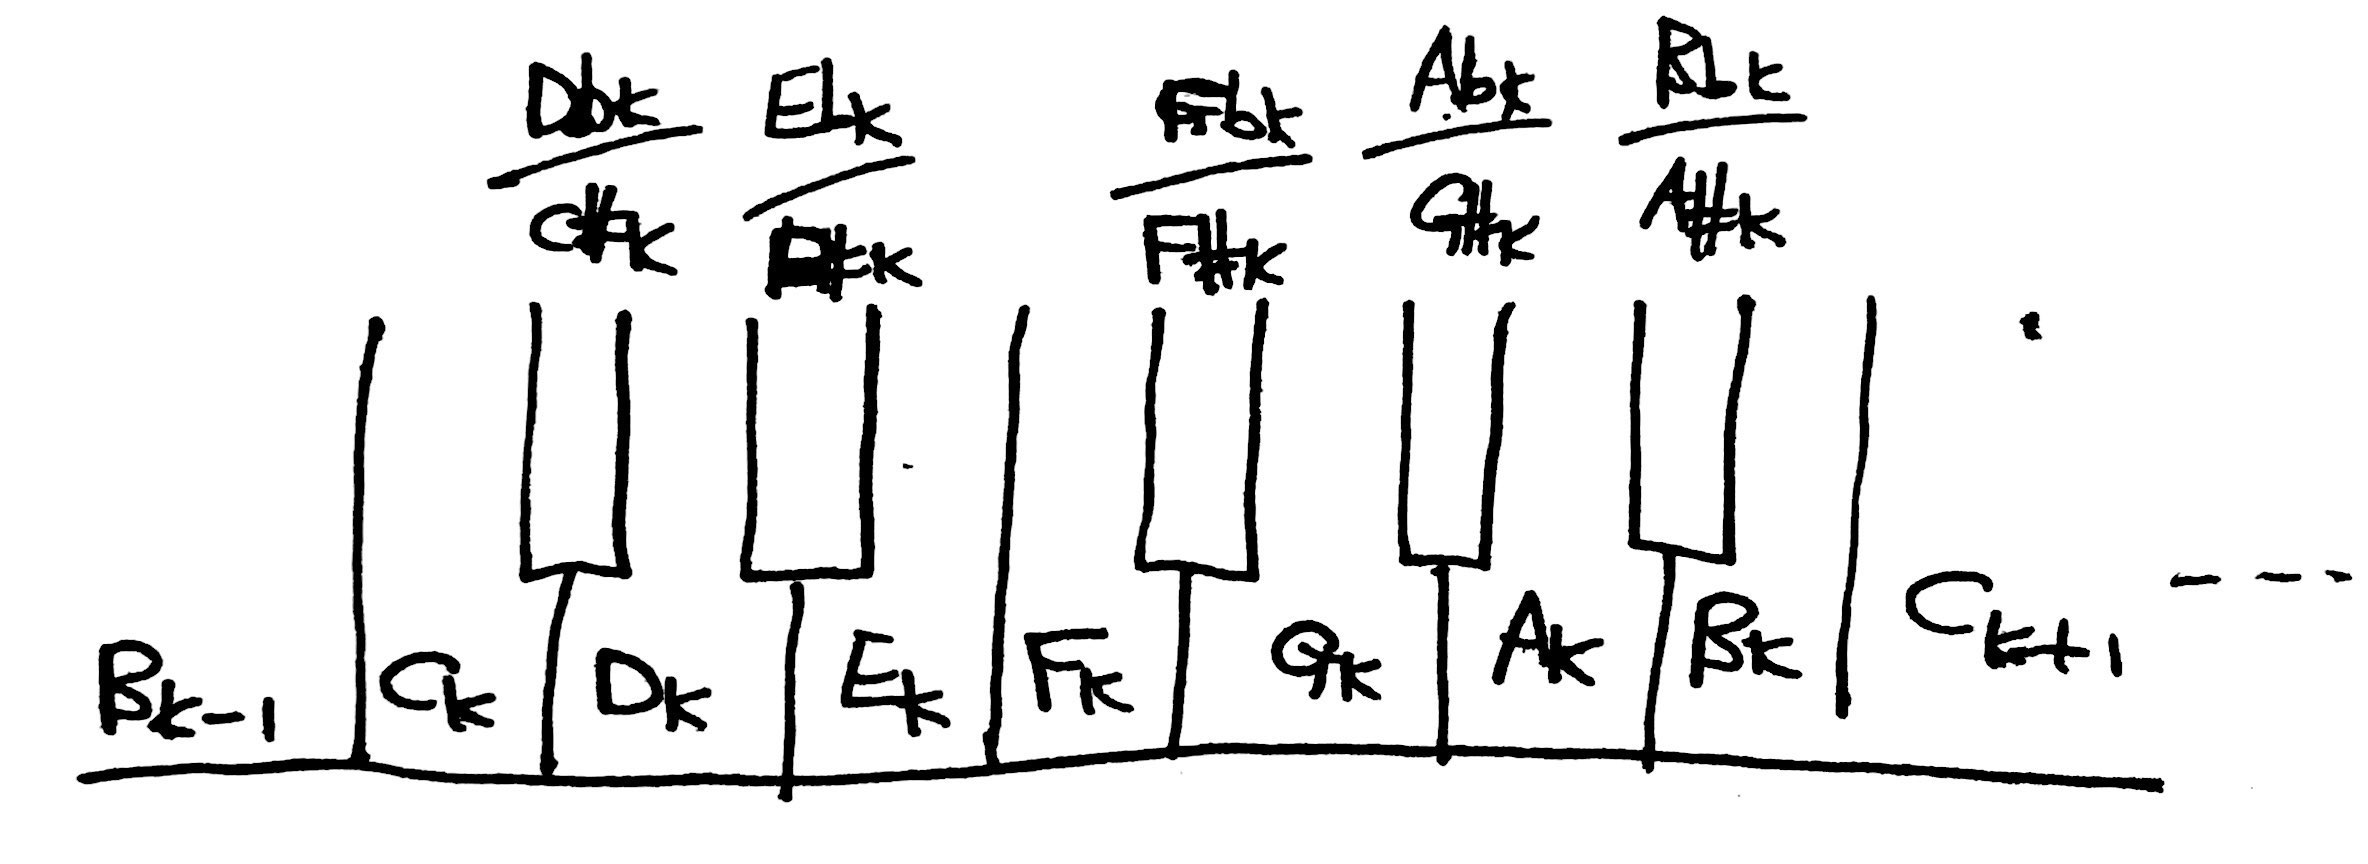
\includegraphics[width=350pt]{figs/piano_spn_tmp.jpg}
\caption{Keyboard illustrating pitches in chromatic scale annotated using SPN}
\label{fig:keyboard-spn}
\end{figure}

We shall constrain our discussion to the context of Western classical music,
since the style which we wish to model lies within this context. A \emph{pitch}
is an abstract concept which is related to the frequency of a musical note.
Formally, if $p,q$ are pitches with corresponding frequencies $\nu_p,\nu_q$,
then if $\nu_q = 2\nu_p$, $p$ and $q$ are said to span an \emph{octave}, with
$q$ an octave above $p$. In Western classical music, each octave is divided into
twelve distinct \emph{note names} (A through G modified by accidentals
\insharp{} or \inflat{}). A note name, such as `B\inflat' (or, equivalently,
A\insharp), is typically thought of as not just a single pitch, but a
\emph{pitch class}, the set of all pitches an integer number of octaves above or
below any pitch with that note name.  Formally, given some reference frequency
$\nu_n$ for a note name $n$, the set of frequencies of the pitches in the pitch
class for $n$ is given by $\set{ 2^k \cdot \nu_n\ |\ k \in \mathbb{Z} }.$

The mapping between pitch and frequency is known as \emph{temperament}, which on
modern instruments is typically \emph{equal}, meaning that the frequency space is
equally divided among the twelve pitches in an octave. More precisely, the
$(k+1)$\textsuperscript{th} note of the chromatic scale with base frequency $\nu_0$ is
given by $2^{k/12}\cdot\nu_0$. As an aside, all recordings of
model outputs in this work were made using equal temperament. Herein
we will work with the abstraction of pitch, ignoring the underlying frequencies
of notes.

To refer to specific pitches, we make use of \emph{scientific pitch notation}
(SPN). Write $N_k$ where $N$ is a note name and $k$ is an octave number. To
ground all the definitions made thus far, we use the standard reference
frequency $\mathrm{A}_4 \triangleq 440\ \mathrm{Hz}$.
Figure~\ref{fig:keyboard-spn} shows the SPN labelling of a chromatic scale. An
\emph{interval} refers to the difference in pitch between two notes. Consecutive
note names are said to be a \emph{semi-tone} apart, and an interval of two
semi-tones is known as a \emph{tone}. Later in this work we shall further
abstract pitch and intervals using MIDI pitch numbering, and further concepts
shall be defined as necessary. In the MIDI tuning standard, $\mathrm{A}_4$
corresponds to pitch number $69$.

Figure~\ref{fig:note-values} shows the musical division of time. Along the left
are the British English names we shall use to refer to note values. The speed at
which a piece is played can be specified by fixing the number of times any of these
note values (most commonly, the crotchet) occur in one minute.

\begin{figure}[H]
\centering
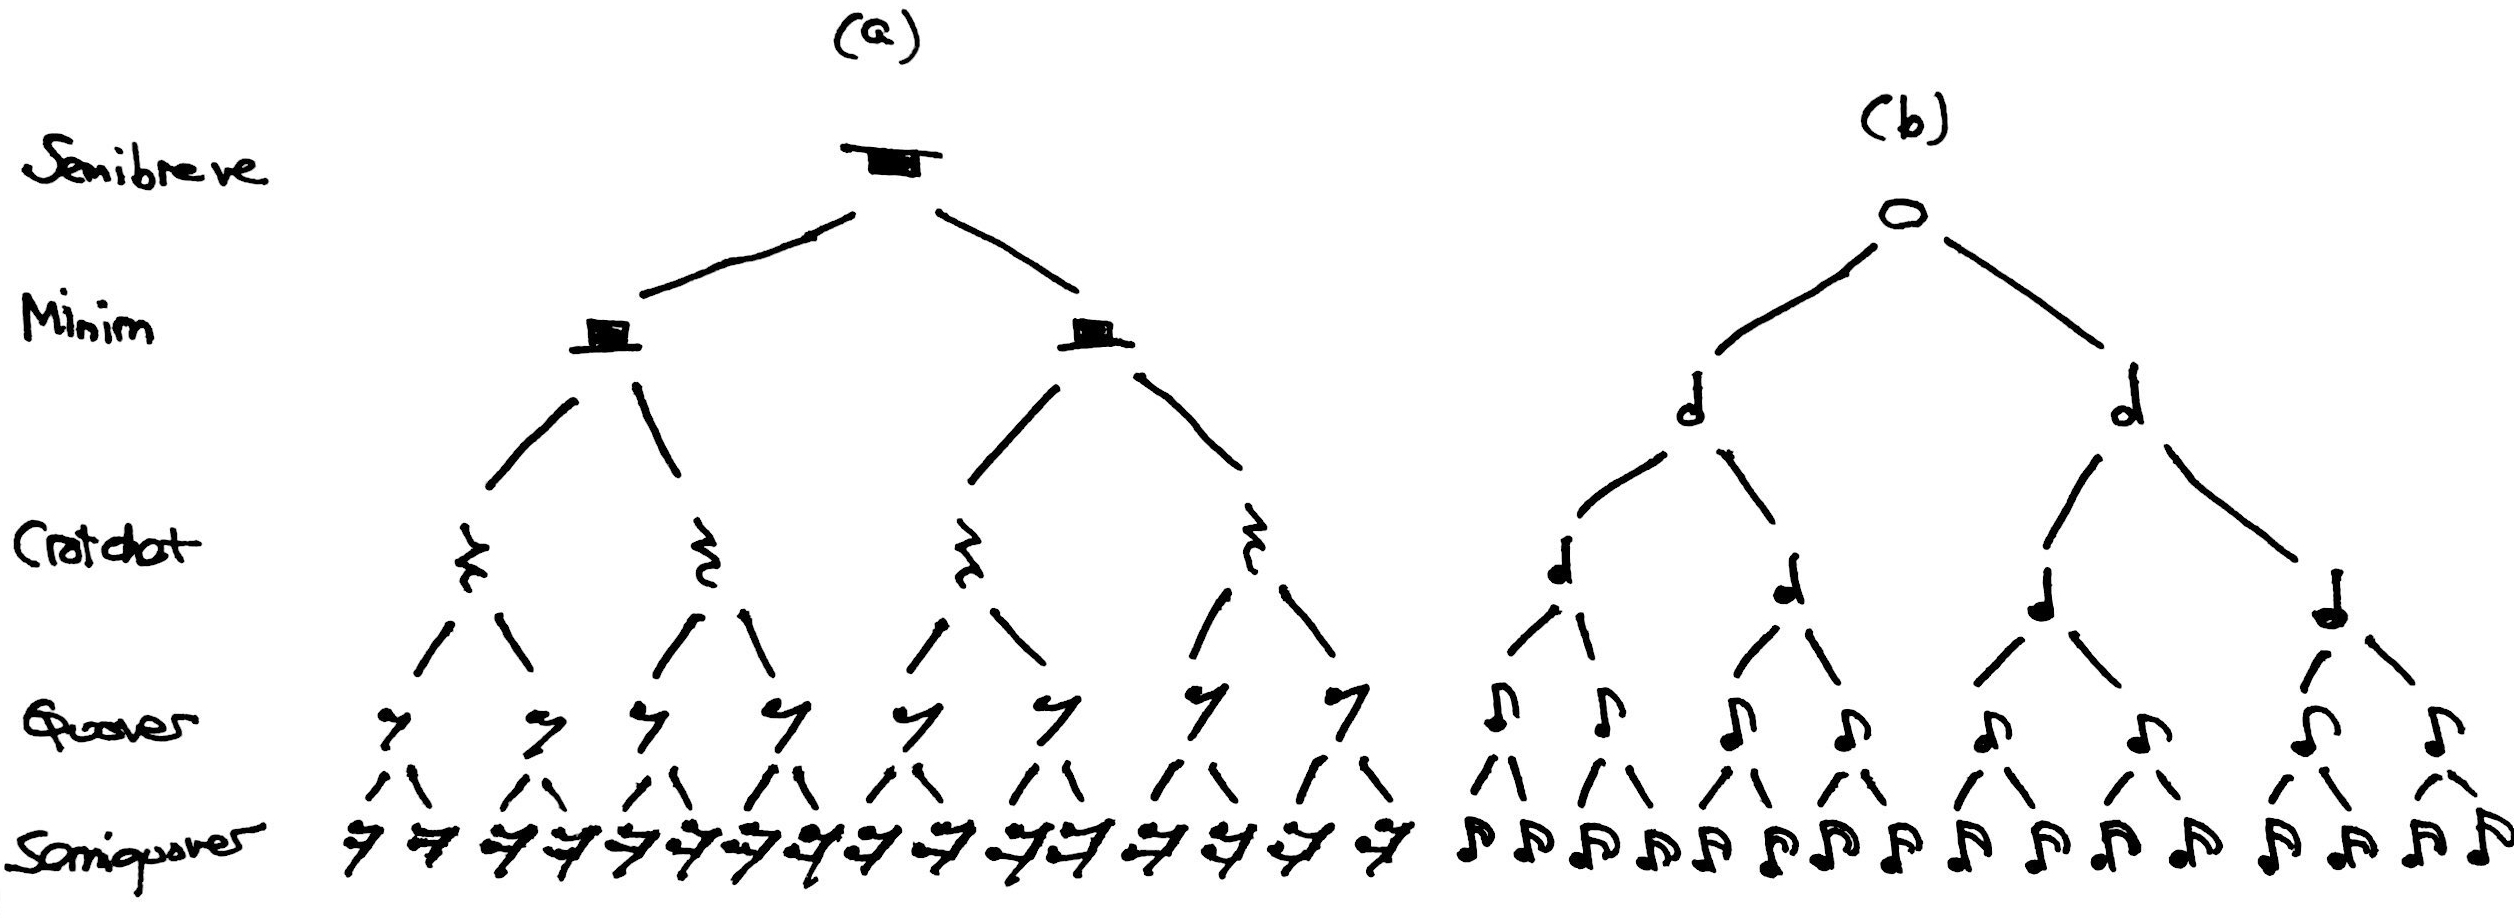
\includegraphics[width=400pt]{figs/note_values_tmp.jpg}
\caption{Notation for Durations of (a) rests and (b) notes}
\label{fig:note-values}
\end{figure}

A dot following a note or rest such as \crotchetDotted{} or \quaverRestDotted{}
indicates that the duration is $1.5$ times the length of its non-dotted
counterpart.

Moreover, Western classical music is typically divided into regular units of
musical time known as \emph{bars}. Both the length of each bar and the regular
rhythmic stress is specified by the \emph{time signature}. The only two time
signatures of concern in this work are \lilyTimeSignature{3}{4} and
\lilyTimeSignature{4}{4}. The numerator indicates the number of \emph{beats} in
a bar, and the denominator the \emph{duration} of each beat. It is important to
be aware that many musical effects are related to the position of a note in the
bar. For example, in \lilyTimeSignature{4}{4}, beats $1$ and $3$ are referred to
as the \emph{strong} beats of the bar and are associated with certain rhythmic
tendencies. We shall exploit this property in the implementation of both
techniques.

\todo tonality???

\subsection{Problem Domain}

In Conklin's 1990 thesis \cite{conklin1990prediction}, he discusses some of the
inherent difficulties in the task of melody generation:

\begin{displayquote}
``Learning plausible continuations in a musical style presents difficulties not
encountered in other domains. In addition to capturing global stylistic rules, a
system must also capture sequential structure, pattern, and repetition within an
individual work.''
\end{displayquote}

Since there are many plausible continuations for a given melodic fragment, this
suggests that probabilistic machine learning techniques will be a useful
approach to take, and casts doubt on the effectiveness of knowledge-based
techniques which attempt to compute exact solutions using hard-coded inference
rules.

\section{Related Work}

\todo Mention GAs.

\subsection{Basic Markov models}

Markov modelling is a technique that has long been applied to music. For a
review, see Ames \cite{ames1989markov}. Basic $n$-gram approaches such as
first-order, higher-order, or indeed variable-order Markov chains over primitive
musical events are all fundamentally limited in that they require an exact match
of a musical context (of some length) in order to make useful predictions. This
is an issue that is addressed by the \emph{multiple viewpoint} approach to
modelling music.

\subsection{Knowledge-based Systems}

Prior to the statistical viewpoint systems investigated in this work, ideas
relating to the method of multiple viewpoints were first applied to music in
1986 by Ebcioğlu in a rule-based system for chorale harmonisation
\cite{ebcioglu1986expert}.  This system used hand-crafted rules written in
first-order logic which were expressed in terms of different viewpoints of the
music. 

\subsection{Multiple Viewpoints}

In 1988, Conklin and Cleary \cite{conklin1988modelling} applied multiple
viewpoints with underlying probabilistic Markov models to modelling Gregorian
chant and simple two-part polyphony. The authors make use of the
\emph{prediction by partial match} (PPM) algorithm \cite{cleary1984ppm} for
smoothing variable-order Markov models, but the escape method used is not
specified.  An ad-hoc, unweighted method is used for combining the predictions
of viewpoints.

Conklin and Witten went on to develop a formalism around multiple viewpoints in
a key 1995 paper \cite{conklin1995viewpoints}. The authors justify discounting
the
\emph{knowledge engineering} approach:

\begin{displayquote}
``There are too many exceptions to any
logical system of musical description, and it will be difficult to ensure the
completeness of an intuited theory. The system will always exclude some valid
pieces. The generations of a theory are bound to reflect the biases of an
engineer; this is the only way they might be called creative.''
\end{displayquote}

With similar reasoning, we shall only consider models which learn from data.  At
this point in time, the convention in the literature became to use ``multiple
viewpoint system'' to refer to \emph{statistical} viewpoint systems with
underlying context models: a convention we shall also adopt.

Many of the ideas in this paper were first published in Conklin's 1990 thesis
\cite{conklin1990prediction}. The notion of separate \emph{long-term} and
\emph{short-term} models in a viewpoint system was introduced in this work.
Conklin also details a principled method for distribution combination, namely
\emph{entropy-weighted arithmetic combination}. 

Among the contributions from his 2005 thesis \cite{pearce2005construction},
Pearce introduces a \emph{geometric} viewpoint combination technique, shown to
outperform its arithmetic counterpart, as well as a method for automatic
viewpoint selection, thereby greatly reducing the selection bias in multiple
viewpoint systems. The work concerns the modelling of melody with a central
focus on \emph{pitch}, as this is deemed to be the most complex of the musical
dimensions.

Whorley's thesis of 2013 \cite{whorley2013phd} deals with the application of
multiple viewpoints to modelling four-part harmony. In addition to improved
algorithms for viewpoint selection, Whorley makes use of a much larger pool of
viewpoints than had previously been available, in particular due to the demands
of modelling four-part harmony.

\subsection{Early Connectionist Approaches}

\begin{figure}[H]
\centering
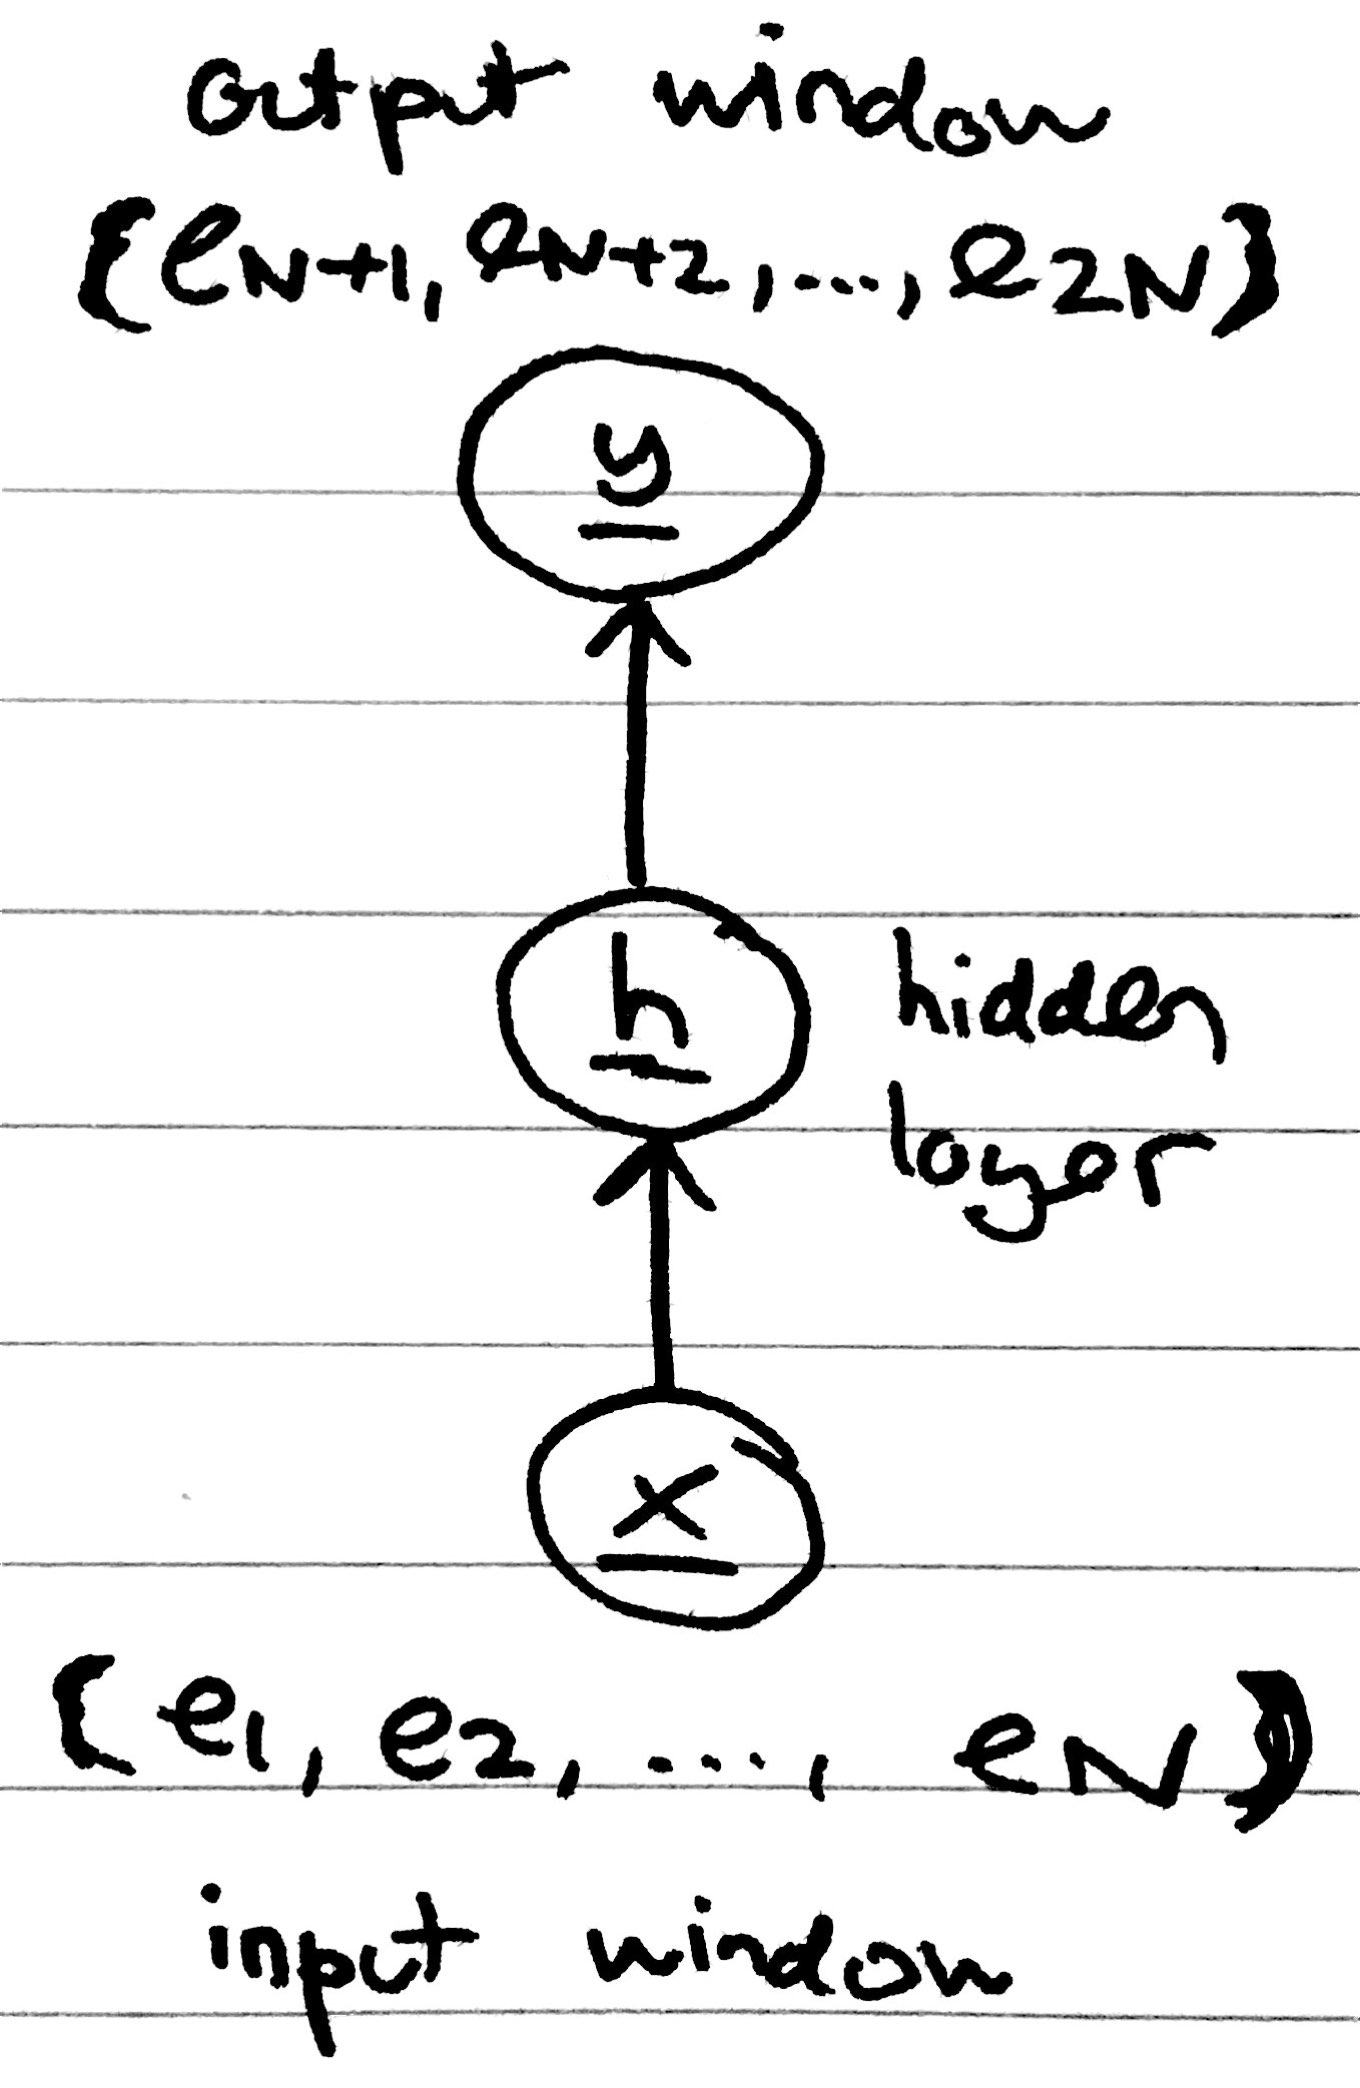
\includegraphics[width=110pt]{figs/windowed_nn_tmp.jpg}
\caption{Windowed feedforward neural network}
\label{fig:windowed-nn}
\end{figure}

Early connectionist approaches to modelling sequential data adapt conventional
feedforward networks to the task by using a finite \emph{windowed} context of
size $N$ and training the network to predict the $N$ events that follow
\cite{todd1989connectionist}. Figure~\ref{fig:windowed-nn} illustrates this
approach.

Observe that, in such an architecture, any common effects between e.g.\ $e_1$
and $e_2$ must be learnt entirely separately from the effects between $e_2$ and
$e_3$, even though there may be a considerable amount of time-invariant
regularity between consecutive events in the sequences of interest. Similarly,
when predicting the output $e_{N+1}^{2N}$, the network will have to learn how to
predict each of these events independently from each other (that is, without
time invariance).  

It can be seen therefore that such networks are very \emph{inefficient} sequence
learners: with a large $N$, vast amounts of training data will be needed and
many parameters to successfully capture any time-invariant effects. Moreover,
with a small $N$ the network will fail to capture any long-term effects.

One solution to this problem is \emph{parameter sharing}, and is central to the
sequence-learning ability of \emph{recurrent neural networks} (RNNs). To quote
the recent text of Goodfellow et al.\ \cite{Goodfellow-et-al-2016}:
\begin{displayquote}
  ``If we had separate parameters for each value of the time index, we could not
  generalise to sequence lengths not seen during training, nor share statistical
  strength across different sequence lengths and across different positions in
  time.''
\end{displayquote}

\subsection{Recurrent Neural Networks}

Recurrent Neural Networks (RNNs), unlike feedforward networks, maintain a
\emph{hidden state} and learn to evolve this hidden state using parameters
specifying transitions which are shared over time. Rumelhart and Hinton et al.\
first showed how to train such networks with backpropagation in 1985
\cite{rumelhart1985learning}. RNNs are clearly a natural tool to apply to
sequence learning. However, basic RNNs are known to suffer from the problem of
\emph{vanishing and exploding gradients}. This problem severely hinders the
ability of basic RNNs to learn long-term dependencies: a capacity which is
crucial in our problem domain.

In 1997, the introduction of the \emph{long short-term memory} (LSTM)
architecture by Hochreiter and Schmidhuber \cite{hochreiter1997long} enabled the
construction of RNNs capable of learning dependencies over many more timesteps
than was previously possible. Today, \emph{gated} architectures such as the LSTM
achieve state-of-the-art results in sequence prediction \cite{zaremba2014recurrent}.

\section{Context of the Work}\label{sec:context-of-work}

In the connectionist literature on modelling music, $n$-gram models are often
used as a baseline approach (e.g.\ \cite{boulanger2012modeling}
\cite{liangbachbot}). However, such $n$-gram models are typically only
models of the surface structure, and sophisticated models such as multiple
viewpoint systems are not usually considered.

Similarly, in the literature on multiple viewpoints, performance comparisons to
modern connectionist techniques are rarely drawn. In particular, to the best of
my knowledge, a direct comparison between multiple viewpoint systems and
recurrent networks does not exist. This work therefore draws an interesting, 
novel comparison between two sophisticated yet contrasting approaches.

\section{Structure}

\todo

\chapter{Preparation}

\section{Choice of Techniques}

Despite the strong performance of multiple viewpoint systems (MVSs) when applied
to music, as discussed in Section~\ref{sec:context-of-work}, they are rarely
used as a baseline approach or brought into comparison with mainstream machine
learning techniques such as neural networks. The reasons for this, we argue, are
three-fold:
\begin{itemize}
  \item Considerable domain-specific knowledge is required to implement a MVS.
  \item The implementation of a MVS from scratch is reasonably involved for a
    baseline approach.
  \item To the best of my knowledge, no open source framework for implementing
    MVSs exists.
\end{itemize}

Recurrent Neural Networks (RNNs), and LSTM networks in particular, are among the
most successful general sequence-learning models in use at this time. Primarily,
therefore, it is the lack of comparison between these two techniques that
motivates this choice. Secondarily, as a by-product of choosing to implement a
general framework for multiple viewpoints, it is my intention that an open
source project that may be of use to researchers for further work can be
released.

I chose to implement the MVS from scratch due to the lack of available
libraries, and based the RNN on an existing library which abstracted away parts
of the implementation that were not of particular interest in this comparison,
such as computing the gradients in the backwards pass of the network.

\section{Starting Point}

Prior to starting this work, I had given a talk on basic $n$-gram approaches to
melody generation using first-order Markov models of melody. This was
accompanied by some code for demonstration purposes. Other than this, I have
not done previous research or implementation in this area. All of the code
written for this project, aside from established libraries, was written from
scratch.

Several courses from the Computer Science Tripos provided background for the
project. The most relevant among these were Information Theory, Artificial
Intelligence, Machine Learning, and, supporting the design of the
evaluation survey, Human Computer Interaction. 

\section{Deliverables}

The success criteria for the project comprise the following deliverables:
\begin{itemize}
  \item A program or tool for importing the corpus in the desired format.
  \item A multiple viewpoint system (MVS) capable of generating melody.
  \item A recurrent neural network (RNN) capable of generating melody.
  \item Quantitative and human evaluation.
\end{itemize}

This chapter concerns the ideas behind the first three of these, along with
a discussion of the research and decisions made prior to implementation.
Chapter~\ref{chap:eval} will discuss the design and implementation of the
human evaluation survey in detail, as well as quantitative evaluation.

\section{Choice of Corpus and Representation}\label{sec:corp-rep}

The chosen corpus was a set of chorale melodies used in the harmonisations of
J.S.\ Bach. The Bach Chorales are a corpus of great interest in the
computational modelling of music: the style is unified, yet with significant
inter-opus variance; it is not too complex, yet not overly simplistic.

Various other musical styles were considered. For example, folk melodies are
often used in this kind of work. These were discarded, since the corpora I
investigated were considered too simplistic to be of interest. Hymn tunes were
also considered; however, aside from there being no readily-available corpora
for this genre, the possibility of bias in the evaluation survey from users being
familiar with the samples was of concern.

An internal format for melody based on a representation used commonly in the
multiple viewpoint system literature (e.g.\ \cite{conklin1995viewpoints}) was
decided on. It was decided that musical time should be quantised with a quantum
of $1/16$\textsuperscript{th} notes (semiquavers), since this is the smallest
note duration encountered in the chosen corpus.

This representation was to be used internally for both the MVS and
RNN implementations. A note $n$ is represented as a tuple $(p,o,d) \in
\mathbb{N}^3$ where $p$ is the MIDI pitch number of $n$, $o$ is the onset 
time, and $d$ is the duration. A melody is then a list of such tuples. Note that
rests are not explicitly represented as events in this encoding.

\section{Overview of Music Generation}\label{sec:gen-models}

A system for music generation need not be probabilistic. Techniques such as
genetic algorithms and rule-based systems are capable of generating output
without modelling a probability distribution over the output space. Following
the reasoning of the previous chapter, however, we shall exclusively consider
probabilistic models. 

\begin{figure}[H]
\centering
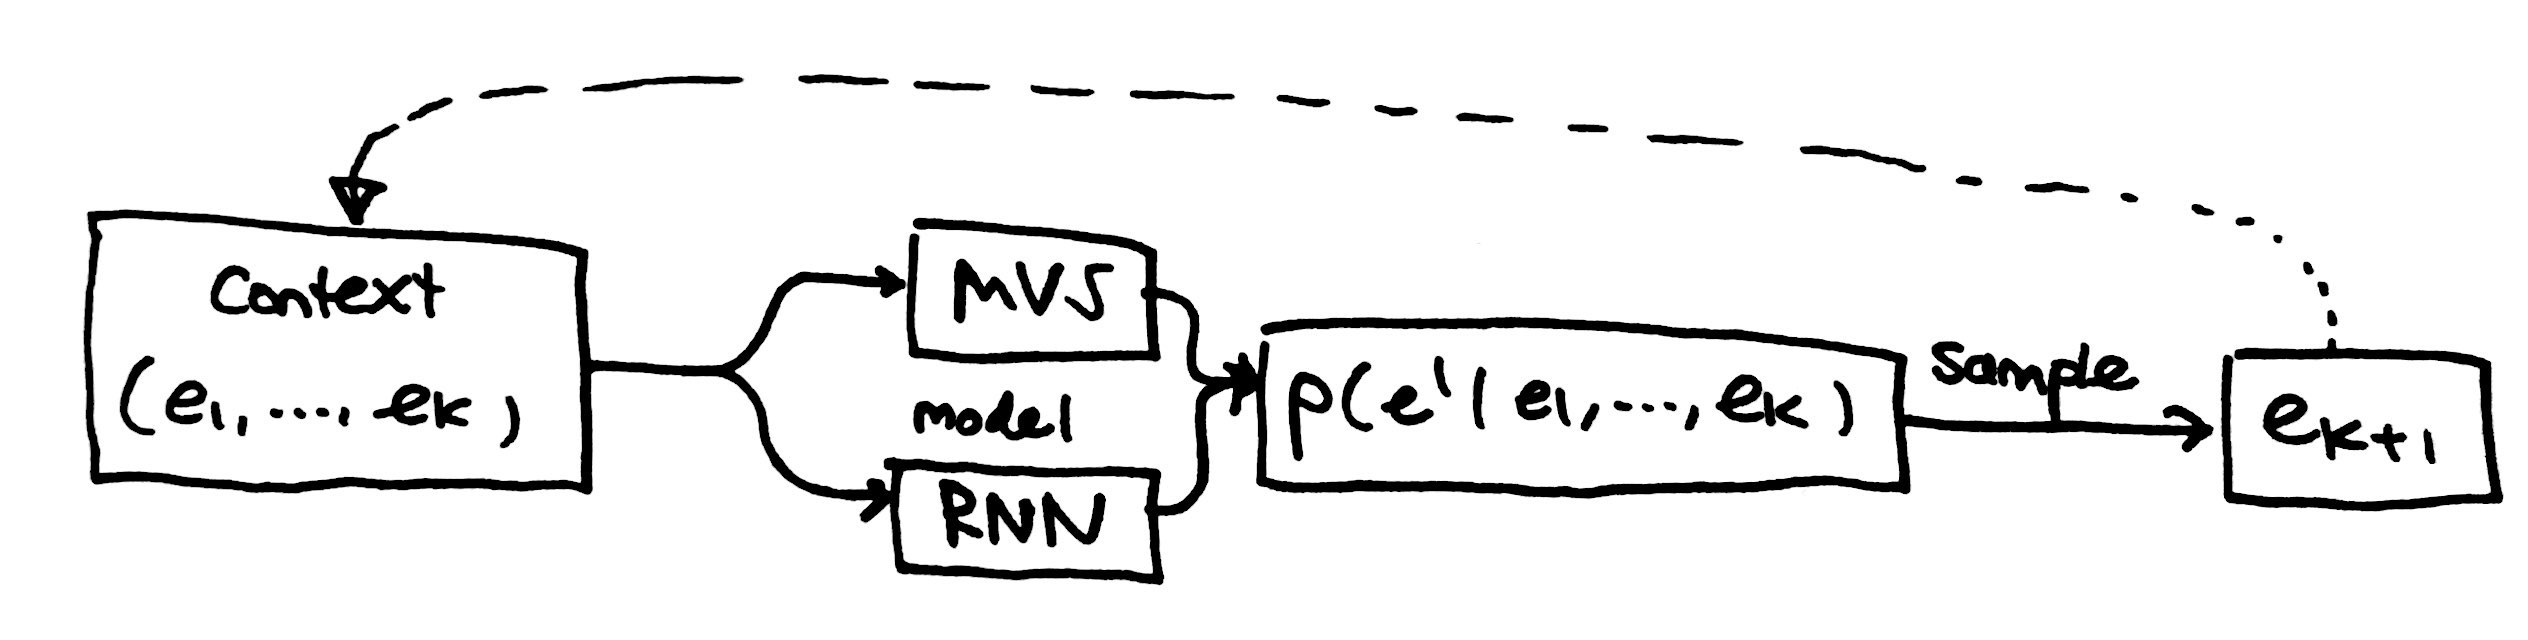
\includegraphics[width=400pt]{figs/high_level_tmp.jpg}
\caption{Overview of probabilistic sequence generation}
\label{fig:seq-gen-overview}
\end{figure}

Any system which models a probability distribution over the data of interest is
said to be a \emph{generative model}. Let $\vect{x} = x_1, \ldots, x_t$ range
over sequences of interest. Then a model which calculates or approximates
$p(\vect{x})$ is a generative model of such sequences.

This distribution is commonly approximated by assuming that each event 
depends only on those that come before it, yielding (\ref{eq:cond-indep}). All the
models we work with will make this assumption of conditional independence. A
high-level overview of the generation process using such models is given in
Figure~\ref{fig:seq-gen-overview}.
\begin{equation}
  p(\vect{x}) = p(x_t | x_{t-1}, \ldots, x_1) p(x_{t-1} | x_{t-2},
  \ldots, x_1) \cdots p(x_1) \label{eq:cond-indep}
\end{equation} 

An even stronger assumption is the \emph{Markov assumption}, which assumes that
we only need to look at a finite context of length $n$ to be able to predict the
future, i.e.
\begin{equation}
  p(x_k | x_{k-1}, \ldots, x_1) \approx p(x_k | x_{k-1}, \ldots, x_{k-n}). 
\end{equation} 

In any case, given some generative model approximating $p(\vect{x})$, we can
\emph{sample} from this distribution to obtain an output sequence from the
model. In the case of models that make the assumption of (\ref{eq:cond-indep}),
we can sample by \emph{random walk}, since the probability of the next event
depends only on those that have been generated thus far. At time $t$, for $t =
1$ to $T$, we sample from:
$$ p(x_t | x_{t-1}, \ldots, x_1) $$
and immediately accept the resulting event $x_t$, appending it to our sample.

While random walk sampling is very efficient, running in $\Theta(T)$ time to
generate a sequence of length $T$, it can sometimes generate solutions
$\vect{x}'$ with low $p(\vect{x}')$. Typically, we want to sample sequences that
our model assigns high probabilities. To mitigate this, one can simply
repeatedly draw samples $\vect{x}'$ by random walk until $p(\vect{x}') > \alpha$
for some threshold $\alpha$: this algorithm is known as \emph{iterative random
walk}.

This project investigates two generative models that approximate $p(\vect{x})$
using the assumption of (\ref{eq:cond-indep}). To generate a candidate
$\vect{x}'$ from these models, we sample from their distributions by means of
(iterative) random walk. The next two sections introduce these models, with a
focus on the underlying theory and decisions made prior to implementation.

\section{Multiple Viewpoint Systems}

In this section, the key theory, algorithms, and data structures underpinning
multiple viewpoint systems are introduced. The notation and formalism is as per
Conklin and Witten \cite{conklin1995viewpoints}. We start by defining some
notation which will be used throughout this section.

\begin{itemize}[itemsep=0mm]
  \item If $\tau$ is a type, then $[\tau]$ is the \emph{syntactic domain} of
    that type: all elements of type $\tau$.   
  \item $S^*$ denotes the set of all sequences drawn from a set $S$.
  \item $e_i^j$ abbreviates the sequence $(e_i,e_{i+1},\ldots,e_{j-1},e_j)$ and
    $()$ the empty sequence.
  \item $s :: e$ denotes the sequence $s$ with event $e$ appended.
  \item $\zeta$ denotes the \emph{event space}, the set of all possible events
    that can occur in sequences of interest. For example, a very simple event
    space for melody might be:
    $$ [\mathrm{pitch}] \times [\mathrm{duration}] \times [\mathrm{onset}]. $$
\end{itemize}

\subsection{Context Models}\label{sec:ctx-model-prep}

The central primitive underlying a multiple viewpoint system is the
\emph{context model}. In general, a context model over some type $\tau$ is a
data structure storing sequences in $[\tau]^*$ together with an inference
procedure predicting distributions over $[\tau]$ given some context in
$[\tau]^*$. The inference procedure in such a model relies on the Markov
assumption, as detailed in Section~\ref{sec:gen-models}.

The context model is initially specialised from example sequences: subsequences
are extracted and stored in the underlying data structure. The inference
procedure later makes predictions by matching inputs contexts against this data
structure. The context models I implement are variable-order Markov models with
some maximum history\footnote{ An $n$\textsuperscript{th} order Markov chain
  makes predictions based on $n$ elements of context. For notational
  convenience, and for consistency with the literature, we generally refer to
  the \emph{history} $h = n+1$ of an $n$\textsuperscript{th} order Markov model.
Such a model stores and models $h$-grams.  } $\hbar$. Such a model can be
thought of as a combination of $\hbar$ Markov models with histories
$1,2,\ldots,\hbar$. 

A known problem with high-order Markov models is their space complexity. A naïve
tabular approach uses $\Theta(|[\tau]|^h)$ space.  In practice, such high-order
models are \emph{sparse}: most $h$-grams are never seen in the training data. A
data structure which exploits this sparsity is the \emph{suffix tree} or
\emph{trie}.  In such a structure, the nodes are events, each with an associated
count, and a path from the root corresponds uniquely to a particular $h$-gram.
Figure~\ref{fig:dur-trie} illustrates this data structure, in this case the trie
supporting a context model over musical durations. 

\begin{figure}[H]
\centering
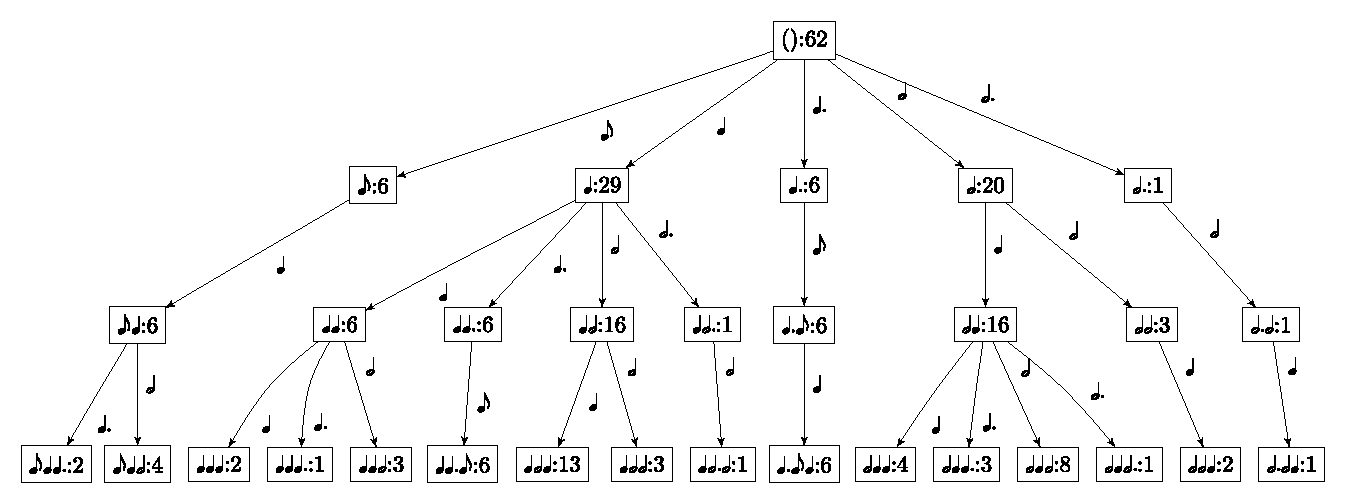
\includegraphics[width=455pt]{figs/duration_vp.pdf}
\caption{Trie for a context model over musical duration with $\hbar = 3$}
\label{fig:dur-trie}
\end{figure}

The algorithm for extracting $h$-grams for a training sequence $e_1^k$ works by
passing a sliding window of size $\hbar$ across the input sequence and
generating $h$-grams in this window of size $1$ through $k$. 

\subsubsection{Inference from Context Models}

Once we have constructed the trie for a context model, we need an algorithm to
perform \emph{inference}. In particular, we want to compute $\mathbb{P}(e' |
e_1^k)$ for some next event $e' \in [\tau]$ and input context $e_1^k \in
[\tau]^*$.

An initial attempt might simply use the maximum likelihood solution to this
problem, which computes the relative frequency of the $h$-gram of interest:
\begin{equation}
  \mathbb{P}(e'|e_1^k) = \frac{ C(e_1^k::e') }{ \sum_{e''} C(e_1^k::e'') }
  \label{eq:ctx-max-like}
\end{equation}
where $C(e_i^j)$ denotes the count associated with $e_i^j$ in the trie, or $0$
if such a node does not exist. Note that all sequences longer than $\hbar$ (and
contexts longer than $\hbar-1$) are implicitly ignored, so $\forall j \in
\mathbb{N}.\ C(e_{k-\hbar-j}^k) = C(e_{k-\hbar+1}^k)$ and
$\mathbb{P}(e'|e_{k-\hbar+1-j}^k) = \mathbb{P}(e'|e_{k-\hbar+2}^k)$.

There are two main problems with this naïve solution. The first is that we want
our models to be \emph{non-exclusive}: all events should be possible, however
improbable. Formally, we require $\forall e' \in [\tau].\ \mathbb{P}(e' | e_1^k)
> 0$. An \emph{exclusive} model would limit the scope for creativity in the
system, and moreover, from a practical standpoint, evaluation metrics such as
\emph{cross-entropy} require calculating log-probabilities: we therefore want to
avoid zero probabilities. This approach, however, fails to guarantee
non-exclusivity.

The second problem with this solution is that it does not deal with \emph{novel
contexts}. In particular, suppose we have not seen the context $e_1^k$. Then,
clearly, the denominator of (\ref{eq:ctx-max-like}) will be zero, which is
equally problematic.

I chose to implement an algorithm which attends to both of these issues:
\emph{prediction by partial match} (PPM) \cite{cleary1984ppm}. The central idea
behind PPM is that, instead of distributing the probability mass entirely among
the exact context matches, as per (\ref{eq:ctx-max-like}), we instead reserve
some amount of the probability mass for as-yet unseen symbols. This reserved
probability mass is known as the \emph{escape probability}. The escape
probability is then distributed recursively among a lower-order model. In this
sense, PPM belongs to the more general class of \emph{backoff smoothing}
algorithms.

Backoff smoothing algorithms are typically formulated recursively, as per
(\ref{eq:ppm-general}).
\begin{equation}\label{eq:ppm-general}
  \mathbb{P}(e' | e_1^k) = \begin{cases}
  \alpha(e'|e_1^k) & C(e' | e_1^k) > 0 \\
\gamma(e_1^k) \cdot \mathbb{P}(e' | e_{(k - \hbar) + 2}^k) & \text{otherwise}
\end{cases} 
\end{equation} 

The choice of escape probability $\gamma(\cdot)$ is known
as the \emph{escape method}: established methods include A, B, C, D, and AX
\cite{pearce2004improved}. PPM A, the method implemented in this work, uses the
following $\alpha$ and $\gamma$ functions:
\begin{align}
  \label{eq:ppm-a-alpha}
  \alpha(e' | e_1^k) &= \frac{ C(e' | e_1^k) }{ 1 + \sum_{e''} C(e'' | e_1^k) }
  \\
  \gamma(e_1^k) &= \frac{ 1 }{ 1 + \sum_{e'} C(e' | e_1^k) }
  \label{eq:ppm-a-gamma}
\end{align}

It is clear from this formulation that all events are assigned some non-zero
probability, meaning that PPM gives rise to non-exclusive models. To see how the
problem of novel contexts is dealt with, consider calculating $\mathbb{P}(e' |
e_1^k)$ for some unseen context $e_1^k$. Since $e_1^k$ is unseen, we have
$\forall e' \in [\tau].\ C(e' | e_1^k) = 0$. Therefore, evaluating
(\ref{eq:ppm-a-alpha}) and (\ref{eq:ppm-a-gamma}), we find $\alpha(e'|e_1^k) =
0$ and $\gamma(e_1^k) = 1$. Thus, for any unseen context, PPM deterministically
backs off to the next lowest-order model. If no match is found for any model,
the recursion bottoms out with a uniform distribution. 

This recursive formulation can be somewhat misleading, as the notation implies
that (\ref{eq:ppm-general}) gives rise to properly normalised probability
distributions. This is in fact not the case. 

\begin{figure}[H]
\centering
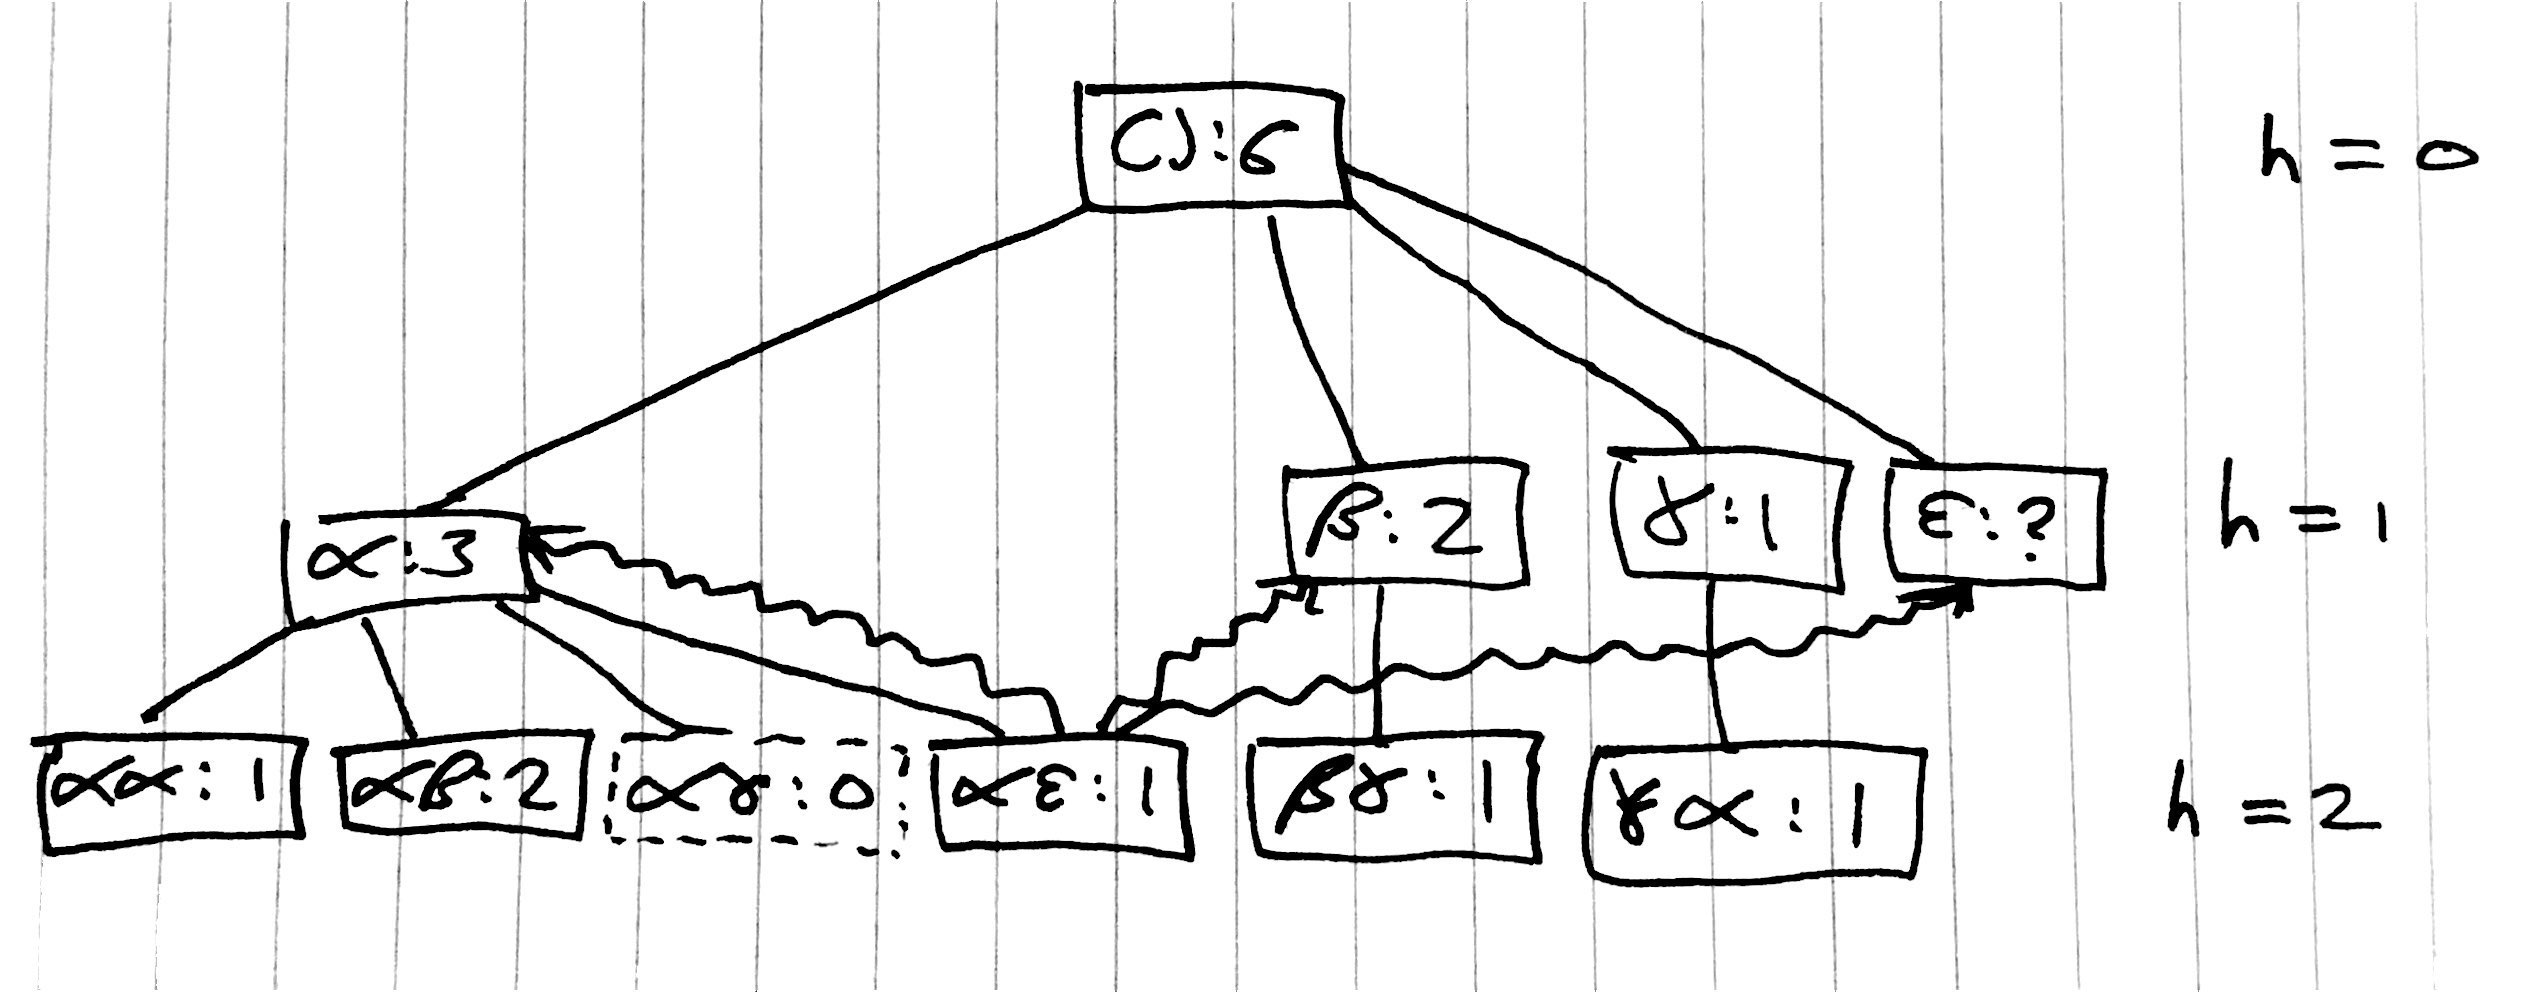
\includegraphics[width=400pt]{figs/problematic_trie_tmp.jpg}
\caption{Trie demonstrating lack of normalisation in standard PPM.}
\label{fig:bad-ppm-trie}
\end{figure}

To see this, consider performing PPM with $\hbar = 2$ over an alphabet $\Sigma =
\set{\alpha,\beta,\gamma}$, and suppose we have seen the training sequence
$(\alpha,\beta,\gamma,\alpha,\alpha,\beta)$.  Figure~\ref{fig:bad-ppm-trie}
illustrates the situation, and includes virtual $\epsilon$-nodes to represent
the escape mass.

The first problem is the escape node at layer $h = 1$. According to
(\ref{eq:ppm-a-gamma}) it should have an effective count of $1$. However, this
yields:
\begin{align}
  \sum_{e \in \Sigma} \mathbb{P}(e) = \frac{3}{7} + \frac{2}{7} + \frac{1}{7} =
\frac{6}{7} \neq 1. 
\end{align} 
The observation to make here is that if \emph{all} symbols in our alphabet have
a non-zero count for any given context, then the escape probability is
redundant. Suppose, then, we set the effective count of this $\epsilon$-node to
zero. Consider the distribution $\mathbb{P}(e|\alpha)$. We can trivially compute
$\mathbb{P}(\alpha|\alpha) = 1/4$ and $\mathbb{P}(\beta|\alpha) = 1/2$, and for
$\gamma$ we escape to find $\mathbb{P}(\gamma|\alpha) = 1/4 \cdot
\mathbb{P}(\gamma)$. However, $\mathbb{P}(\gamma) < 1$, so
$\mathbb{P}(e|\alpha)$ is not normalised. The problem here is that the escape
mass for the node labelled $\alpha\epsilon$ is distributed among all the symbols
at layer $h = 1$ in the trie, when in reality we can only ever escape to
$\gamma$.

There are two typical solutions for this lack of normalisation in PPM: in
earlier work, authors often simply compute an improper distribution and later
normalise it (e.g.\ \cite{conklin1990prediction}). A more sophisticated and less
wasteful solution which reasons about the possible $h$-grams that can be escaped
to is known as PPM with \emph{exclusion} \cite{pearce2004improved}. I chose to
implement exclusion for the context models in this work.

\subsection{Viewpoints}\label{sec:mvs-formalism}

One possible approach to modelling music would be to form a context model over
the entire event space $\zeta$.  Recall that $\zeta = [\tau_1] \times [\tau_2]
\times \cdots \times [\tau_n]$ is the cartesian product of many types. Aside
from being computationally expensive, this approach is severely limited in its
predictive power, since it requires an \emph{exact match} of the musical context
to make useful predictions: that is, there is no ability of the system to
\emph{generalise} to unseen contexts. This problem is illustrated in
Figure~\ref{fig:generalise}.

\begin{figure}[H]
\centering
\input{figs/generalise.pdf_tex}
\caption{Melodic fragments illustrating importance of generalisation}
\label{fig:generalise}
\end{figure}

An obvious approach to allow the system to generalise would be to model some or
all of the $\tau_i$ \emph{independently}. To see why this might be useful,
consider that while there is certainly some correlation between e.g.\ pitch and
duration, much of the rhythmic regularity in a particular corpus is independent
of the pitch of the notes: thus, it is likely to be fruitful to model duration
independently of any of the other musical attributes. Fragment (b) of
Figure~\ref{fig:generalise} motivates modelling pitch
independently of duration.

Further, complex languages such as music can be viewed using many abstract
interpretations. To give a simple example, one can consider the \emph{melodic
contour} with domain $\set{-1,0,1}$ which indicates whether a melody is falling,
stationary, or rising. A more directly useful abstract interpretation is the
\emph{melodic interval}, which exploits the fact that intervalic patterns in
most music capture regularity that is \emph{invariant} to the absolute pitch.
Fragment (c) of Figure~\ref{fig:generalise} motivates this interpretation.
Modelling regularity in such abstract domains and transforming the predictions
back into predictions over the concrete $\tau_i$ might therefore further allow
the system to generalise.  

\emph{Viewpoints} allow us to model music from these different points of view:
namely, we can model the individual $\tau_i$, as well as abstract
interpretations and combinations thereof. We now proceed to set up the formalism
of multiple viewpoints.

First, allow $\tau$ to range over types other than just the \emph{basic types}
that make up the component types of $\zeta$. We call these non-surface types
\emph{derived types}: the abstract interpretations derived from the surface
$\tau_i$. 

\textbf{Definition}. A \emph{viewpoint} modelling a type $\tau$ is:
\begin{enumerate}[label=\arabic*., itemsep=0mm]
  \item a partial function $\Psi_\tau : \zeta^* \rightharpoonup [\tau]$,
    together with
  \item a context model of sequences in $[\tau]^*$.
\end{enumerate}

The function $\Psi_\tau$ for a type $\tau$ is known as the \emph{projection}
function for $\tau$: it projects out the last element of type $\tau$ from some
surface event stream $e_1^k \in \zeta^*$, if such an element exists. Note that,
for convenience, we shall frequently refer to viewpoints simply by the type they
model. 

Viewpoints, as we have defined them, can clearly model individual surface and
derived types independently. While this is useful, we still need to be able to
model the correlation between basic attributes.

\textbf{Definition}. A \emph{product type} $\tau_1 \otimes \cdots \otimes
\tau_n$ between $n$ types $\tau_1, \ldots, \tau_n$ is itself a type $\tau$ with
$[\tau] = [\tau_1] \times \cdots \times [\tau_n]$. 

For a product type $\tau = \tau_1 \otimes \cdots \otimes \tau_n$:
$$ \Psi_\tau(e_1^k) \triangleq
\begin{cases}
  \langle\Psi_{\tau_1}(e_1^k), \ldots, \Psi_{\tau_n}(e_1^k)\rangle & \forall i
  \in \set{1,\ldots,n}.\
  \Psi_{\tau_i}(e_1^k)\downarrow \\
  \bot & \text{otherwise.}
\end{cases}
$$

Viewpoints over product types are known as \emph{linked viewpoints}. 

Note that one can also make use of \emph{threaded viewpoints}: those defined
only at certain fixed intervals in a sequence. However, these are considered out
of scope for this work.

In order to train a viewpoint over type $\tau$, we need to provide the
underlying context model with sequences in $[\tau]^*$. To obtain such sequences
from surface events, we simply iterate the projection function $\Psi_\tau$ to
give a function $\Phi_\tau : \zeta^* \rightarrow [\tau]^*$ which we call the
\emph{lifting} function, defined as follows:
\begin{align*}
  \Phi_\tau(()) &\triangleq () \\
  \Phi_\tau(e_1^k) &\triangleq \begin{cases}
    \Phi_\tau(e_1^{k-1})::\Psi_\tau(e_1^k) & \Psi_\tau(e_1^k)\downarrow \\
    \Phi_\tau(e_1^{k-1}) & \text{otherwise.}
  \end{cases}
\end{align*}

In practice, we shall see that it is typically easier to implement $\Phi_\tau$
directly. However, formally, it is cleaner to specify $\Psi_\tau$ to define a
particular viewpoint.

Now consider a viewpoint over a type $\tau$ derived from some surface type
$\tau'$. This viewpoint will predict distributions over the abstract type
$\tau$, but we actually need a distribution over the concrete $\tau'$. 

The process of transforming a distribution from the abstract domain to the
concrete is given limited treatment in the literature. Whorley
\cite{whorley2013phd} notes that this is effectively ``using the partial
function $\Psi_\tau$ in reverse on each of the viewpoint elements.'' We argue
that the surface context is also needed to perform this task, and will refer to
this process as \emph{reification}, specified by a partial function $\rho :
\zeta^* \times \mathrm{dist}(\tau) \rightharpoonup \mathrm{dist}(\tau')$, where
$\mathrm{dist}(\tau)$ denotes the set of probability distributions over a type
$\tau$. This will be discussed further in Chapter~\ref{chap:impl}.

\subsection{Combining Viewpoint Predictions}\label{sec:vp-comb}

Recall that, given some musical context $e_1^k \in \zeta^*$, the goal is to
predict the next event $e_{k+1} \in \zeta$ where $\zeta = [\tau_1] \times \cdots
\times [\tau_n]$.  A collection of viewpoints that performs this task is known
as a \emph{multiple viewpoint system} (MVS). 

A MVS decomposes this task by predicting $e_{k+1}$ componentwise. Out of all the
viewpoints in the system, consider just those viewpoints capable of predicting
some $\tau_i$. At each timestep, given the context $e_1^k$, $N$ of these
viewpoints will \emph{activate}, meaning they predict a distribution for
$\tau_i$. This section concerns techniques for the combination of $N$ such
distributions to form an overall prediction. In particular, we consider
\emph{weighted} schemes as these are widely used in the literature and known to
perform better than unweighted schemes \cite{pearce2004combining}.

The premise of weighted schemes for viewpoint combination is that viewpoints
that are more `confident' in their predictions should be given higher weights.
Since the Shannon entropy of a viewpoint's distribution is a metric of overall
uncertainty, we use weights that are monotonically non-increasing as a function
of distribution entropy.

Suppose we have $N$ distributions over a type $\tau$. Suppose further that there
is some canonical ordering of $[\tau]$, such that we can pick out the
$j$\textsuperscript{th} member. Now, let $p_i(j)$ denote the probability
assigned to $j$\textsuperscript{th} element by the $i$\textsuperscript{th} of the
$N$ distributions. We want to combine these predictions to produce some overall
distribution with
probabilities $p(j)$.

A general weighted arithmetic scheme combines the predictions as follows:
$$
  p(j) = \frac{ \sum_{i = 1}^N w_i p_i(j) }{ \sum_{i = 1}^N w_i }.
$$

The Shannon entropy of the $i$\textsuperscript{th} distribution is given by:
$$ H(i) = - \sum_{j = 1}^{|[\tau]|} p_i(j) \log_2 p_i(j) $$
with maximum value $H_{\mathrm{max}} = \log_2{ |[\tau]| }$. Now define the
\emph{normalised entropy} $\hat{H}(i)$ as:
$$ \hat{H}(i) \triangleq \begin{cases}
  H(i)/H_{\mathrm{max}} & H_{\mathrm{max}} > 0 \\
  1 & \text{otherwise.}
\end{cases} $$

In previous work this quantity has been called the \emph{relative entropy};
here, we use \emph{normalised entropy} so as to avoid confusion with the
Kullback-Leibler distance, which is also known by this name.

Finally, so that we can favour distributions with lower $\hat{H}$, we introduce
an exponential bias $b \in \mathbb{R}_0^+$:
$$ w_i = \hat{H}(i)^{-b}. $$

Note that we do not restrict $b$ to integer values, as is commonly done in the
literature \cite{whorley2013phd}. Pearce \cite{pearce2004improved} introduces a
new method for combining viewpoint predictions which outperforms arithmetic
schemes: namely, a \emph{weighted geometric mean}:
$$ p(j) = \frac{1}{Z} \left( \prod_{i = 1}^N p_i(j)^{w_i} \right)^{ \frac{1}{
\sum_{i = 1}^N w_i }} $$
where $Z$ is a normalisation constant, and the $w_i$ are calculated as before.

\begin{figure}[H]
\centering
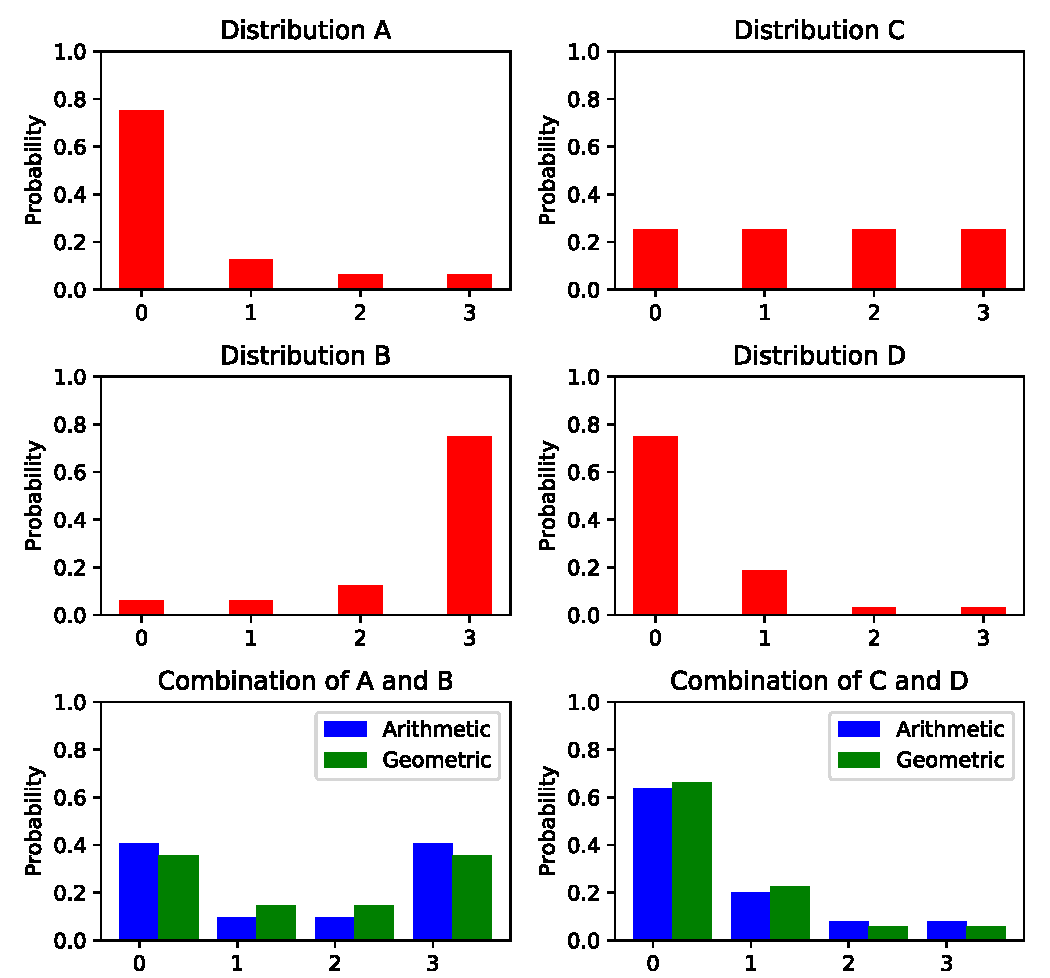
\includegraphics[width=400pt]{figs/dist_comb.pdf}
\caption{Plots illustrating effect of distribution combination schemes ($b = 2$)}
\label{fig:dist-comb-plot}
\end{figure}

Figure~\ref{fig:dist-comb-plot} shows the effect of using these two schemes on
some example distributions. It can be seen that a very low probability
prediction from one distribution has considerably more bearing with the
geometric scheme. Note also that when combining distributions $C$ and $D$, since
$D$ has much lower entropy (and thus greater certainty), it has considerably
more effect on the overall result under both schemes.

I chose to first implement the arithmetic scheme as a baseline approach and
later implement the geometric scheme.

\subsection{MVS Architecture}\label{sec:mvs-arch}

\begin{figure}[H]
\centering
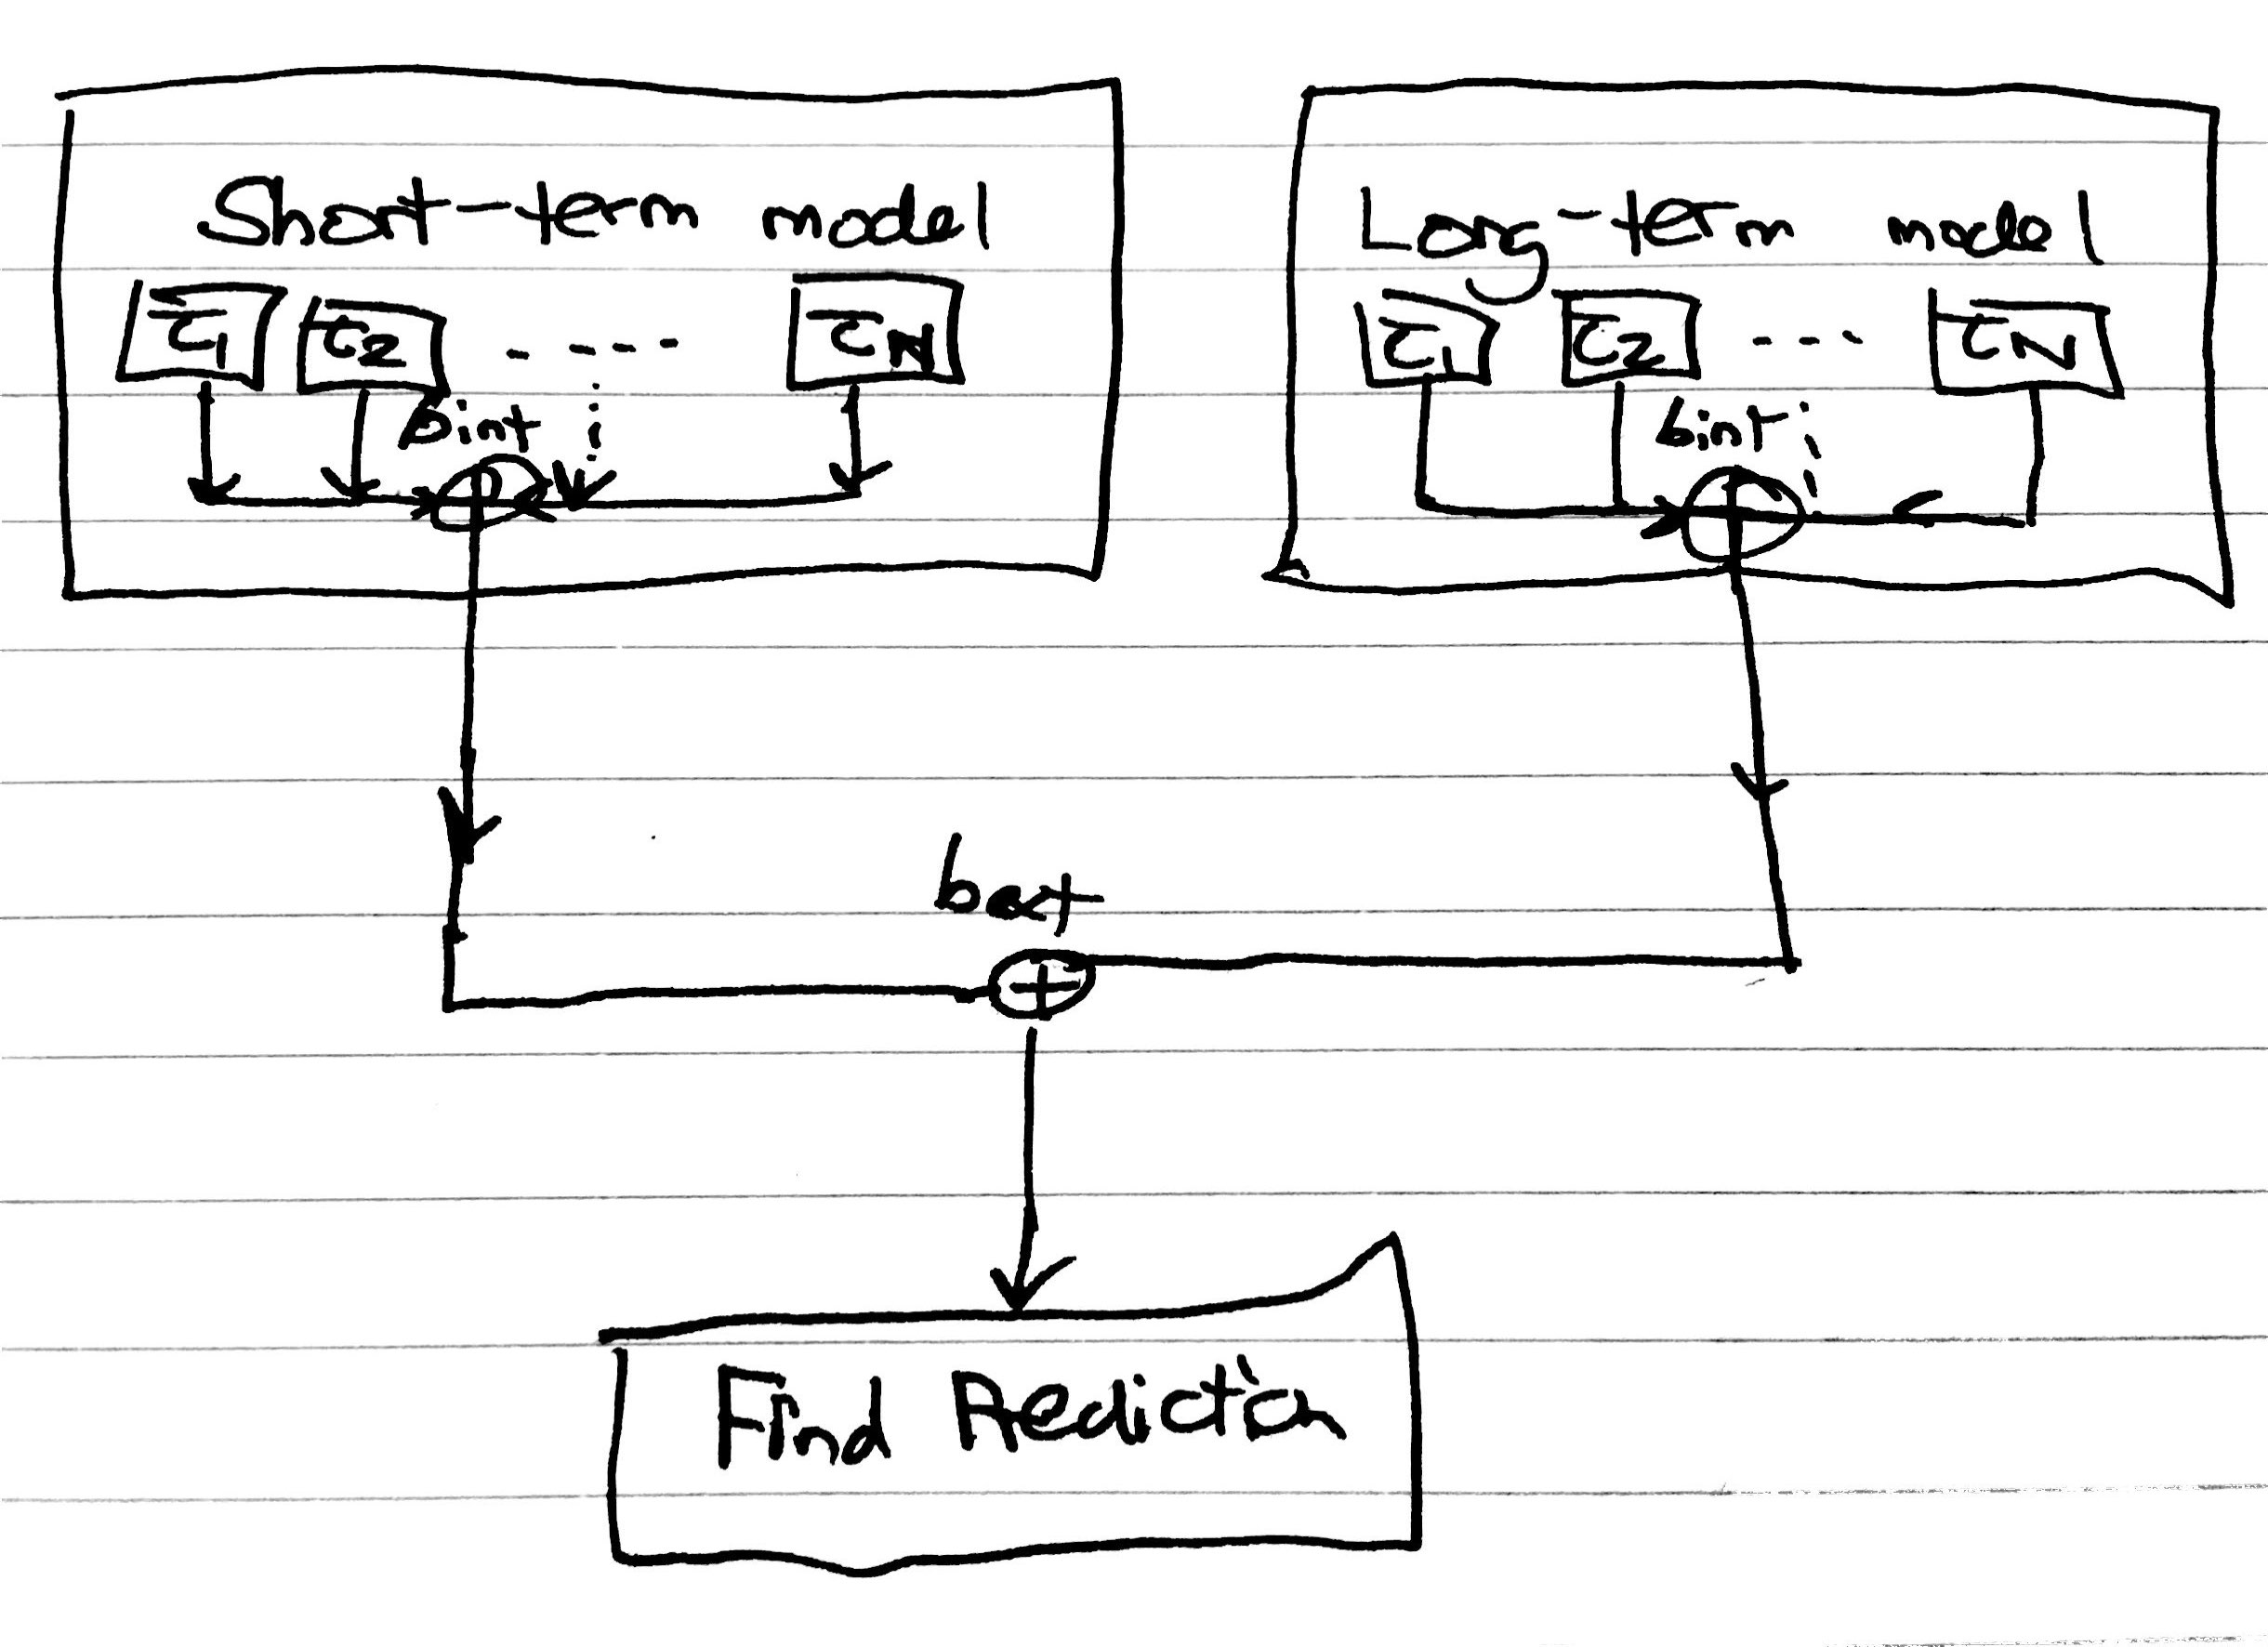
\includegraphics[width=250pt]{figs/mvs_arch_tmp.jpg}
\caption{Typical MVS architecture}
\label{fig:mvs-arch}
\end{figure}

For successful sequence prediction, it is necessary to capture both
intra-sequence and inter-sequence regularity: that is, the \emph{short-term}
effects \emph{local} to a particular sequence, and the \emph{long-term} effects
common through the entire corpus.  This is especially true of music, and indeed
the chorales, where entire melodic fragments are often re-used within a given
chorale melody.

In a conventional MVS architecture, this is achieved explicitly by using
entirely separate \emph{long-term} and \emph{short-term} models. The long-term
model is trained on the entire corpus, and the short-term model just on the
sequence being predicted or generated. Figure~\ref{fig:mvs-arch} illustrates
this architecture: viewpoint combination is indicated by $\oplus$, and is
performed as per Section~\ref{sec:vp-comb}.

In order to keep the number of hyperparameters under control, the following
architectural constraints are often enforced (and indeed, are in this work):
\begin{itemize}
  \item The same set of viewpoints $\set{\tau_1, \ldots, \tau_N}$ is used in both
    the long-term and short-term model. 
  \item The viewpoints in the long-term model all have the same order bound
    $h_l$. Similarly, those in the short-term model all have order bound $h_s$.
  \item The viewpoint combination within each of these two models is performed
    using the same bias parameter $b_{\mathrm{int}}$ and the combination of the
    short-term and long-term predictions using a separate bias parameter
    $b_{\mathrm{ext}}$.
\end{itemize}

\section{Recurrent Neural Networks}\label{sec:rnn-intro}

Recurrent neural networks can be formulated as a dynamical system with a state
evolving over time. Given an initial state $\vect{h}_0$ and input data
$\vect{x}_t \in \mathbb{R}^m$, the hidden state $\vect{h}_t \in \mathbb{R}^n$ of
a RNN evolves as per (\ref{eq:dyn-sys}) for $t \in \mathbb{N}$.
\begin{equation}
  \vect{h}_t = f(\vect{h}_{t-1}, \vect{x}_t; \vect{\theta})
  \label{eq:dyn-sys}
\end{equation} 

The output
$\vect{o}_t$ may then be a function of the hidden state $\vect{h}_t$, or indeed
a function of both the state $\vect{h}_t$ and input vector $\vect{x}_t$. The key
observation to make from (\ref{eq:dyn-sys}) is that the same parameters
$\vect{\theta}$ are used at each iteration of $f$. 

We can usefully represent such a network as a \emph{computational graph}. Figure
\todo uses this representation and illustrates the operation of
\emph{unfolding} a recurrence in a computational graph.

\todo Graph unfolding figure here.

In a basic RNN, the choice of $f$ is a simple neural network unit: a
nonlinearity (such as the hyperbolic tangent or logistic sigmoid function)
applied to an affine transformation \cite{zaremba2014recurrent}. Using
$[\vect{u},\vect{v}] \in \mathbb{R}^{m+n}$ to denote the concatenation of
vectors $\vect{u} \in \mathbb{R}^m$ and $\vect{v} \in \mathbb{R}^n$: 
$$f(\vect{h}_{t-1}, \vect{x}_t) = \sigma(\vect{W}[\vect{h}_{t-1}, 
\vect{x}_t] + \vect{b})$$ 
where $\vect{W} \in \mathbb{R}^{(m+n) \times n}$, and $\vect{b} \in
\mathbb{R}^n$. 

The next section explains how we can train recurrent networks in general, and
then proceeds to explore some of the problems due to this simple choice of $f$.

\subsection{Training Recurrent Networks}\label{sec:rnn-train}

The algorithm typically used for training a RNN, known as \emph{backpropagation
through time} (BPTT), applies the standard backpropagation algorithm to the
unfolded computational graph for our RNN. That is, we calculate the derivative
of the cost function with respect to the weights in our network \emph{at each
timestep}. Since the parameters are shared across time, we then sum the gradient
contributions from each timestep and update the weights accordingly by gradient
descent.

Note that training such a network is expensive: supposing we unfold the graph up
to $T$ timesteps, we have to compute the entire forward pass through the network
in $\Theta(T)$ time before gradients can be calculated. Moreover, this cannot be
parallelised, since the computation at timestep $t$ depends on
$\vect{h}_{t-1}$, the result of the computation at the previous timestep.

Even in a RNN that is \emph{spatially} shallow (i.e.\ with a
single layer at each timestep), unfolding the computational graph results in a
graph that is very deep: the network itself is \emph{temporally deep}. With the
choice of $f$ in a basic RNN, the repeated composition of an affine
transformation and nonlinearity can exhibit highly nonlinear behaviour. While
this can be desirable, granting the network much expressive power, training such
networks can be problematic. 

\begin{figure}[H]
\centering
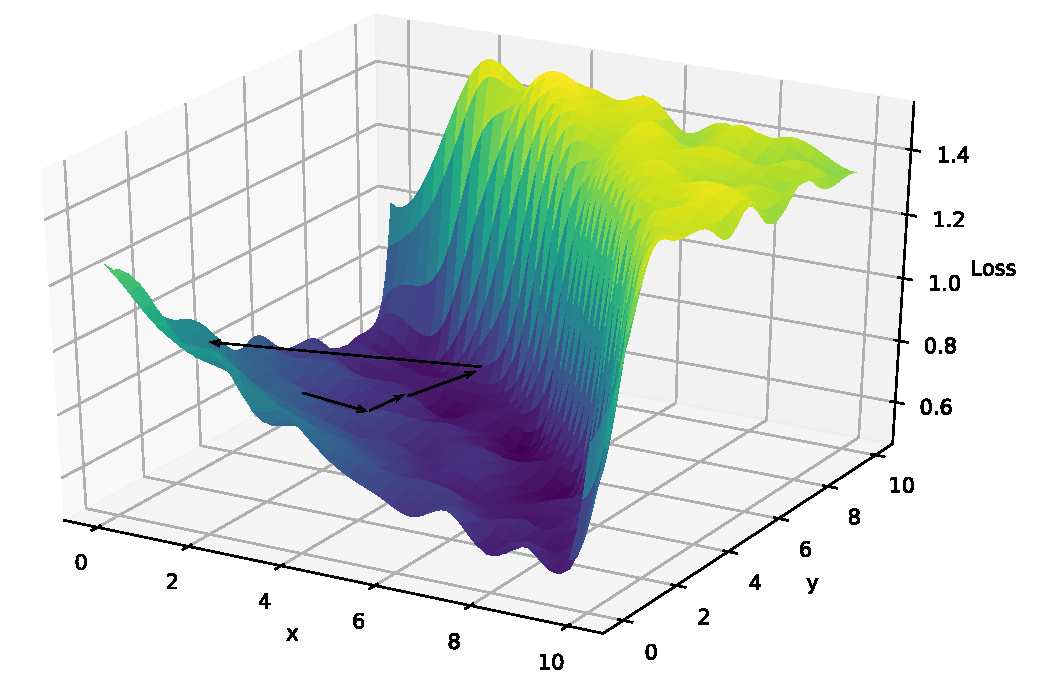
\includegraphics[width=400pt]{figs/exploding_gradients.pdf}
\caption{Illustrative embedding of loss surface with exploding gradients}
\label{fig:exploding-grad}
\end{figure}

One such problem in deep networks is that the high-dimensional surface of our
loss function with respect to the weights can exhibit sharp ``cliffs'' where the
gradient is very large \cite{Goodfellow-et-al-2016}: this is known as the
\emph{exploding gradient problem}, illustrated in
Figure~\ref{fig:exploding-grad}. The negative effects of this problem on
training can, however, largely be mitigated by \emph{clipping} the norm of the
gradient to some maximum value during training.

\subsubsection{Long-term dependencies}

A more insidious problem with basic recurrent networks is the \emph{vanishing
gradient problem}. This is caused not only by the network being very deep, but
in particular by the repeated application of $f$ with the same parameters at
each timestep.

Here, we follow the illustrative treatment of Goodfellow et al.\
\cite{Goodfellow-et-al-2016} and refer to Hochreiter and Schmidhuber
\cite{hochreiter1997long} for a deeper treatment. This argument makes several
simplifying assumptions, but clearly illustrates how the problem might arise in
a simpler setting.

Suppose we simplify the function composition in a neural network to simply apply
matrix multiplication (with no inputs, biases, or nonlinearities). The
recurrence relation: 
$$ \vect{h}_t = \vect{W}^\top \vect{h}_{t-1} $$ 
describes the evolution of such a network. A straightforward induction shows:
$$ \vect{h}_t = (\vect{W}^t)^\top\vect{h}_0 $$
and, supposing that $\vect{W}$ has an eigendecomposition of the form:
$$ \vect{W} = \vect{Q}\vect{\Lambda}\vect{Q}^\top $$
with orthogonal $\vect{Q}$ (i.e.\ $\vect{Q}\vect{Q}^\top = \vect{Q}^\top\vect{Q}
= \vect{I}$), the recurrence can be further simplified to:
$$ \vect{h}_t = (\vect{Q}^\top \vect{\Lambda}^t \vect{Q}) \vect{h}_0. $$
As $t \rightarrow \infty$, any eigenvalues with magnitude less than $1$ will
vanish, and those with magnitude greater than $1$ will explode. The problem of
vanishing and exploding gradients comes from the fact that gradients through the
graph of a such a (simplified) network are \emph{also} scaled according to
$\vect{\Lambda}^t$ \cite{Goodfellow-et-al-2016}.

Complex languages such as music require a good predictor to learn long-term
dependencies in sequences. However, if the gradient vanishes in this manner as
we calculate gradients further back in time, then gradient descent will
experience an exponential slow-up in learning such dependencies. Eventually,
we will also encounter numerical problems with gradients of sufficiently small
magnitude. For this reason, learning long-term dependencies with basic RNNs is
considered intractable.

\subsection{Long Short-Term Memory}\label{sec:lstm-prep}

In 1997, Hochreiter and Schmidhuber discovered a radically different RNN
architecture known as \emph{long short-term memory} (LSTM)
\cite{hochreiter1997long}. Despite the superficial complexity of this
architecture, it is based on a simple fundamental idea which is used to achieve
constant gradient flow through time, thereby enabling LSTM networks to learn
long-term dependencies over many timesteps. The idea is to maintain additional
state known as the \emph{cell state} which flows through the network with only
minor \emph{linear}, \emph{pointwise} interactions, protected by structures
known as gates. 

There are in fact many variants of LSTM: we largely follow Zaremba et al.\
\cite{zaremba2014recurrent} in both notational conventions and LSTM design.
Before introducing LSTMs in detail, we shall first define some notation and
introduce the notion of deep recurrent networks in general.

In a deep recurrent network, information is not only processed horizontally
through time, but also vertically through $L$ hidden layers ($L > 1$). We use a
homogeneous state representation with all states in $\mathbb{R}^n$, including
all input and output vectors. 

Let subscripts denote timesteps and superscripts denote layers so that
$\vect{h}_t^l \in \mathbb{R}^n$ denotes the state at time $t$ in layer $l$. In
order to represent input events $x_t$ drawn from an alphabet $\Sigma$ as vectors
in $\mathbb{R}^n$, we use an embedding $E : \Sigma \rightarrow \mathbb{R}^n$
which is either learned through pre-training or learned together with the
weights for the network. Let $\vect{h}_t^0 = E(x_t)$ denote the input vector at
time $t$ and take $\vect{h}_t^L$ as the output vector at time $t$.

We can now specify a RNN with a deterministic transition function from previous
to current states:
$$ \delta : \vect{h}_t^{l-1}, \vect{h}_{t-1}^l \rightarrow \vect{h}_t^l $$
so a basic RNN as described in Section~\ref{sec:rnn-intro} can be specified as:
$$ \delta(\vect{h}_{t-1}^l, \vect{h}_t^{l-1}) = f(\vect{W}^l_x [\vect{h}_{t-1}^l,
\vect{h}_t^{l-1}] + \vect{b}^l_x) $$
where $\vect{W}^l_x \in \mathbb{R}^{2n \times n}$, $\vect{b}^l_x \in
\mathbb{R}^n$, and $f \in \set{ \sigma, \mathrm{tanh} }$ is a nonlinearity.

Typically, in sequence prediction, the output state $\vect{h}_t^L$ at time $t$
is fed into a densely connected layer to obtain an output vector $\vect{o}_t \in
\mathbb{R}^{|\Sigma|}$:
$$ \vect{o_t} = \vect{W}_y \vect{h}_t^L + \vect{b}_y $$
where $\vect{W}_y \in \mathbb{R}^{n \times |\Sigma|}$ and $\vect{b}_y \in
\mathbb{R}^{|\Sigma|}$. 

Treating $\vect{o}_t$ as log-probabilities, we can obtain a probability
distribution over output symbols $y_t \in \Sigma$ with a softmax activation on
this layer:
$$ p(y_t) = \mathrm{softmax}(\vect{o}_t) $$
where for a vector $\vect{z} \in \mathbb{R}^n$, $\mathrm{softmax}(\vect{z})$ is
given by:
$$ \mathrm{softmax}(\vect{z})_i = \frac{ e^{z_i} }{ \sum_{j = 1}^n e^{z_j} }. $$

Figure~\ref{fig:deep-rnn-arch} illustrates the general architecture of a deep
RNN. The merging of arrows denotes \emph{vector concatenation}. We refer to the
units $A_t^l$ as \emph{cells}, specified by the transition function $\delta$.
Note that weight sharing occurs across time, but each layer has its own
parameters. This makes sense since each layer processes data of a (semantically)
different type. The initial state $\vect{h}_{\mathrm{init}}^l$ for the cells in
the $l$\textsuperscript{th} layer is typically set to $\vect{0}$ or initialised
randomly. 

\begin{figure}[H]
\centering
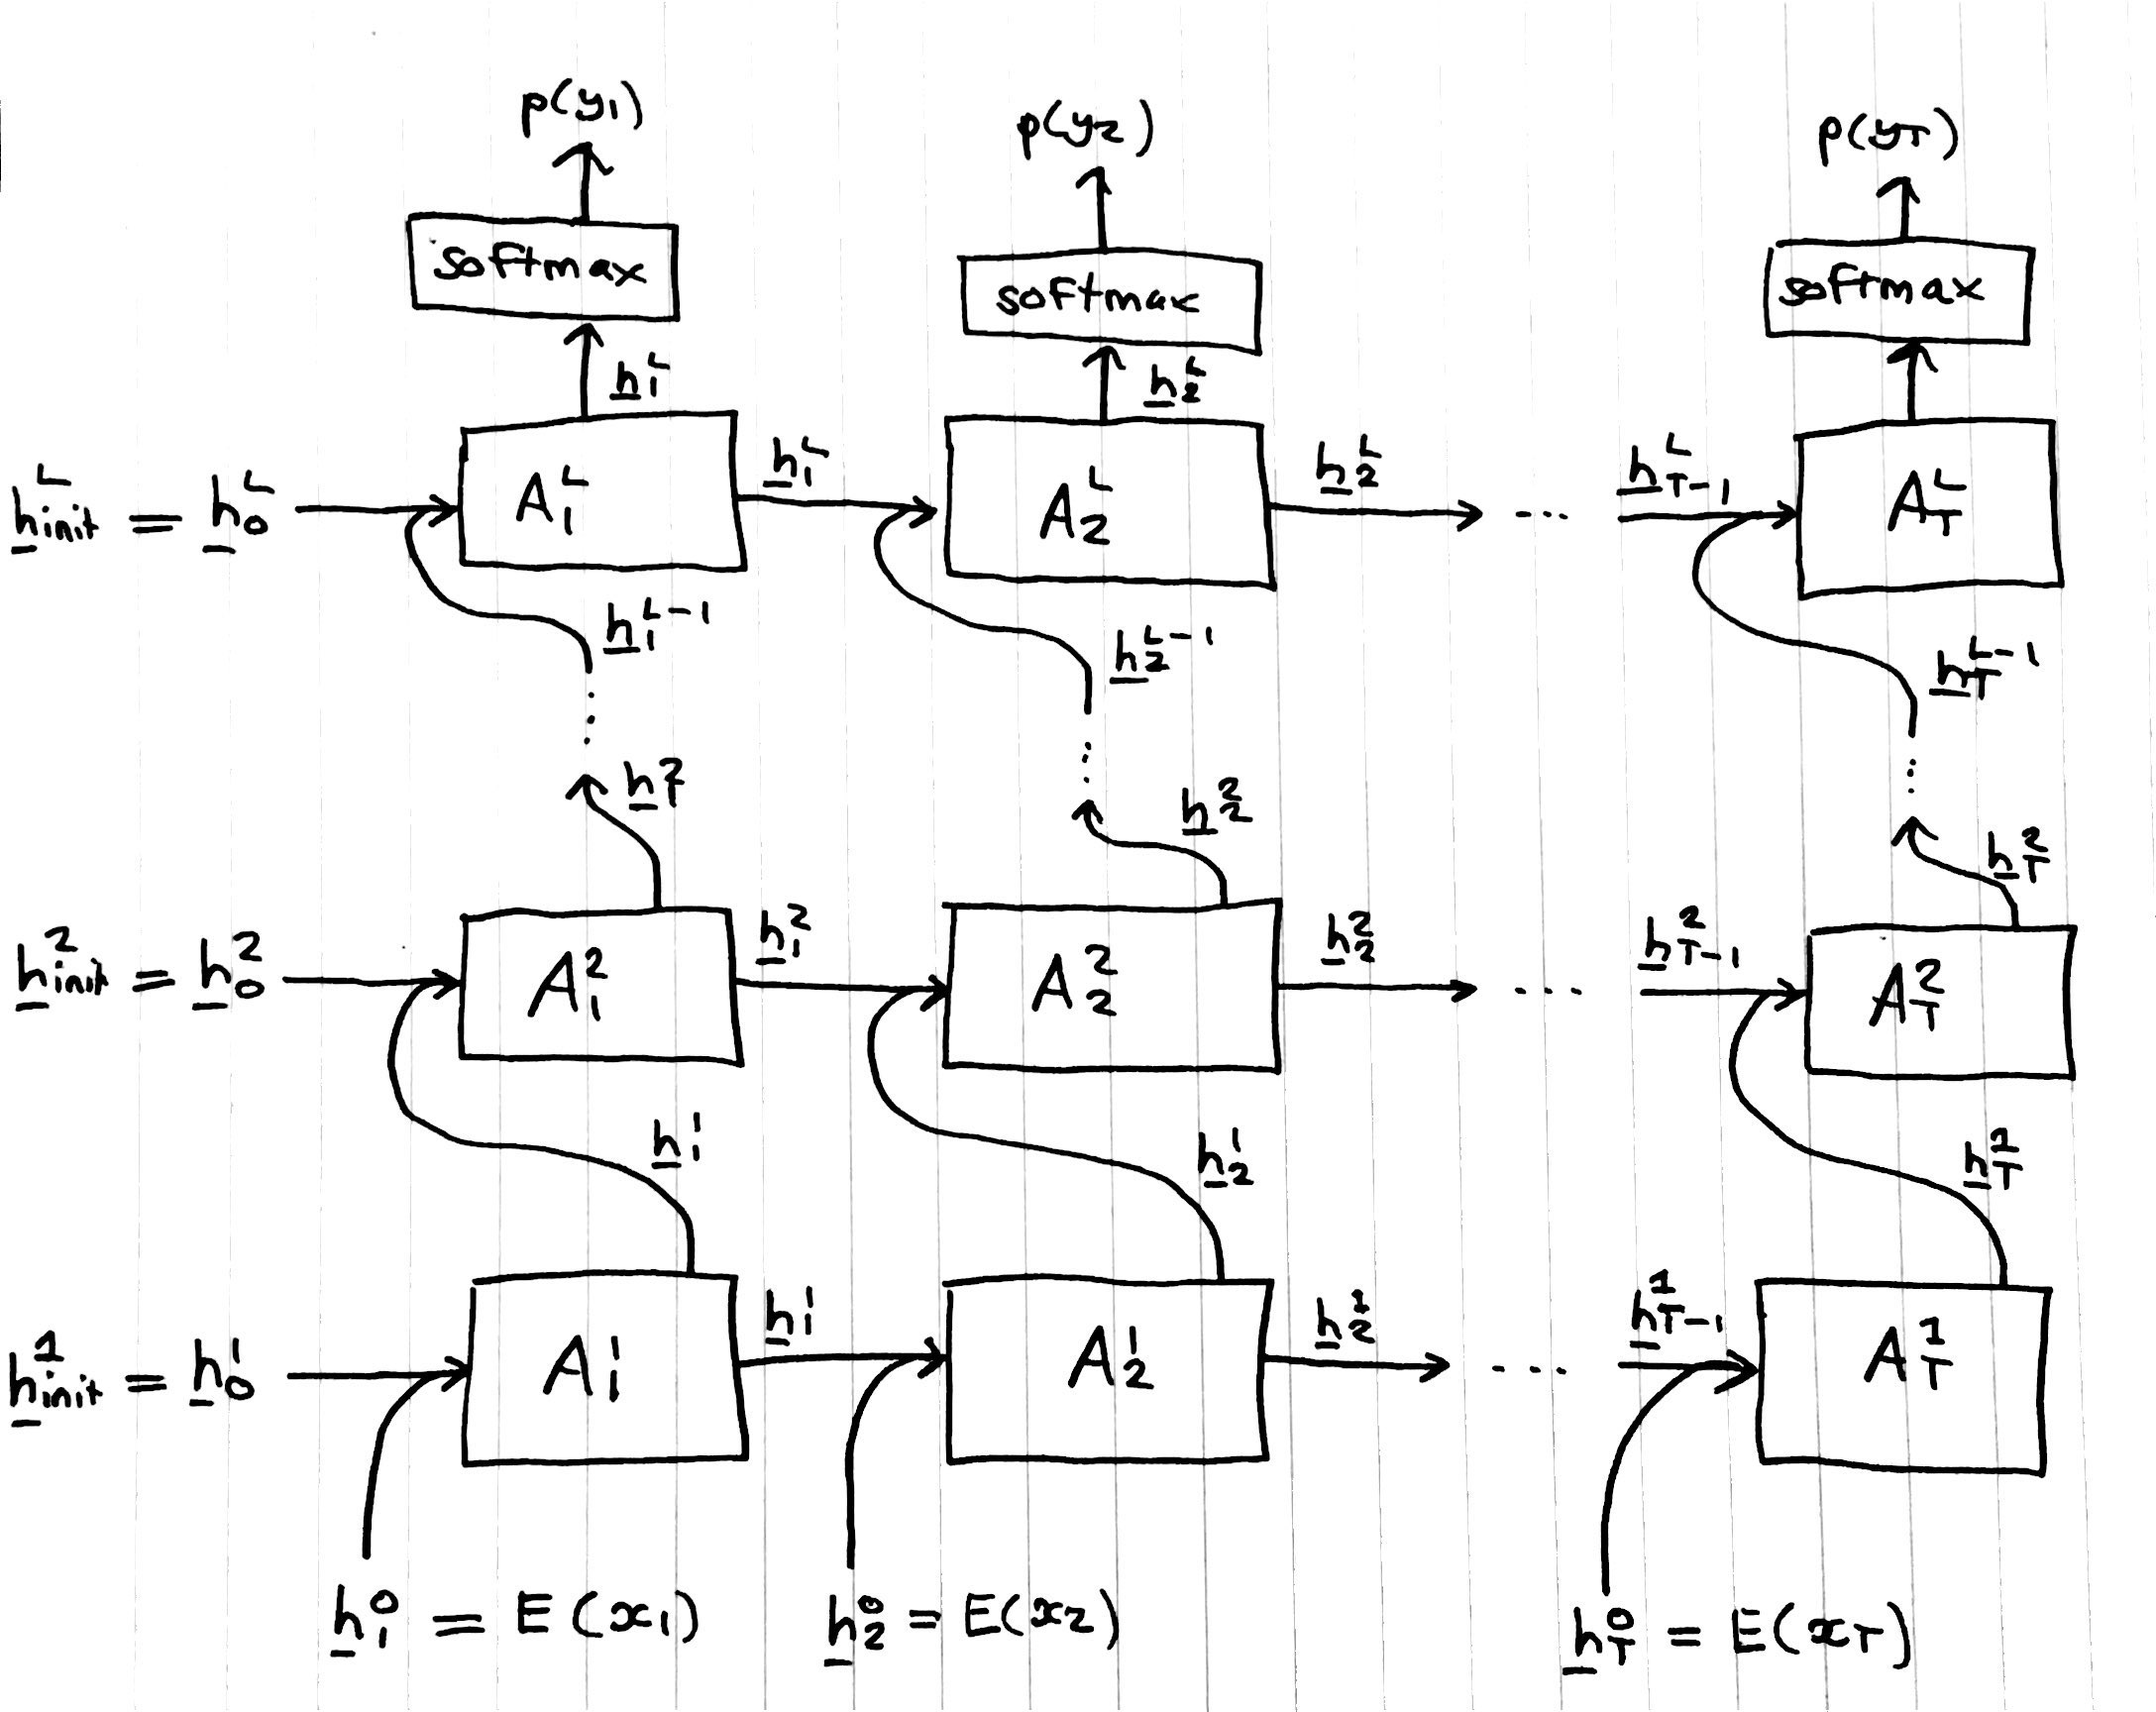
\includegraphics[width=350pt]{figs/deep_rnn_tmp.jpg}
\caption{Flow of information in deep RNN}
\label{fig:deep-rnn-arch}
\end{figure}

We now have the necessary machinery to introduce long short-term memory cells in
the context of deep recurrent networks. LSTM cells replace the $A_t^l$ in the
network with a complex structure centered around carefully protecting the
\emph{cell state}: an additional state vector $\vect{c}_t^l$ that allows data to
flow through many timesteps without undergoing complex non-linear information
morphing as in the case of $\vect{h}_t^l$.

Therefore, our $\delta$ function for LSTMs needs to specify the temporal
transformation of $\vect{c}_t^l$ in addition to the hidden state
transformations:
$$ \delta_{\mathrm{LSTM}} : \vect{h}_{t-1}^l, \vect{h}_t^{l-1}, \vect{c}_{t-1}^l
\rightarrow \vect{h}_t^l, \vect{c}_t^l. $$

The flow of information through an LSTM network is shown in
Figure~\ref{fig:deep-lstm-arch}.

\begin{figure}[H]
\centering
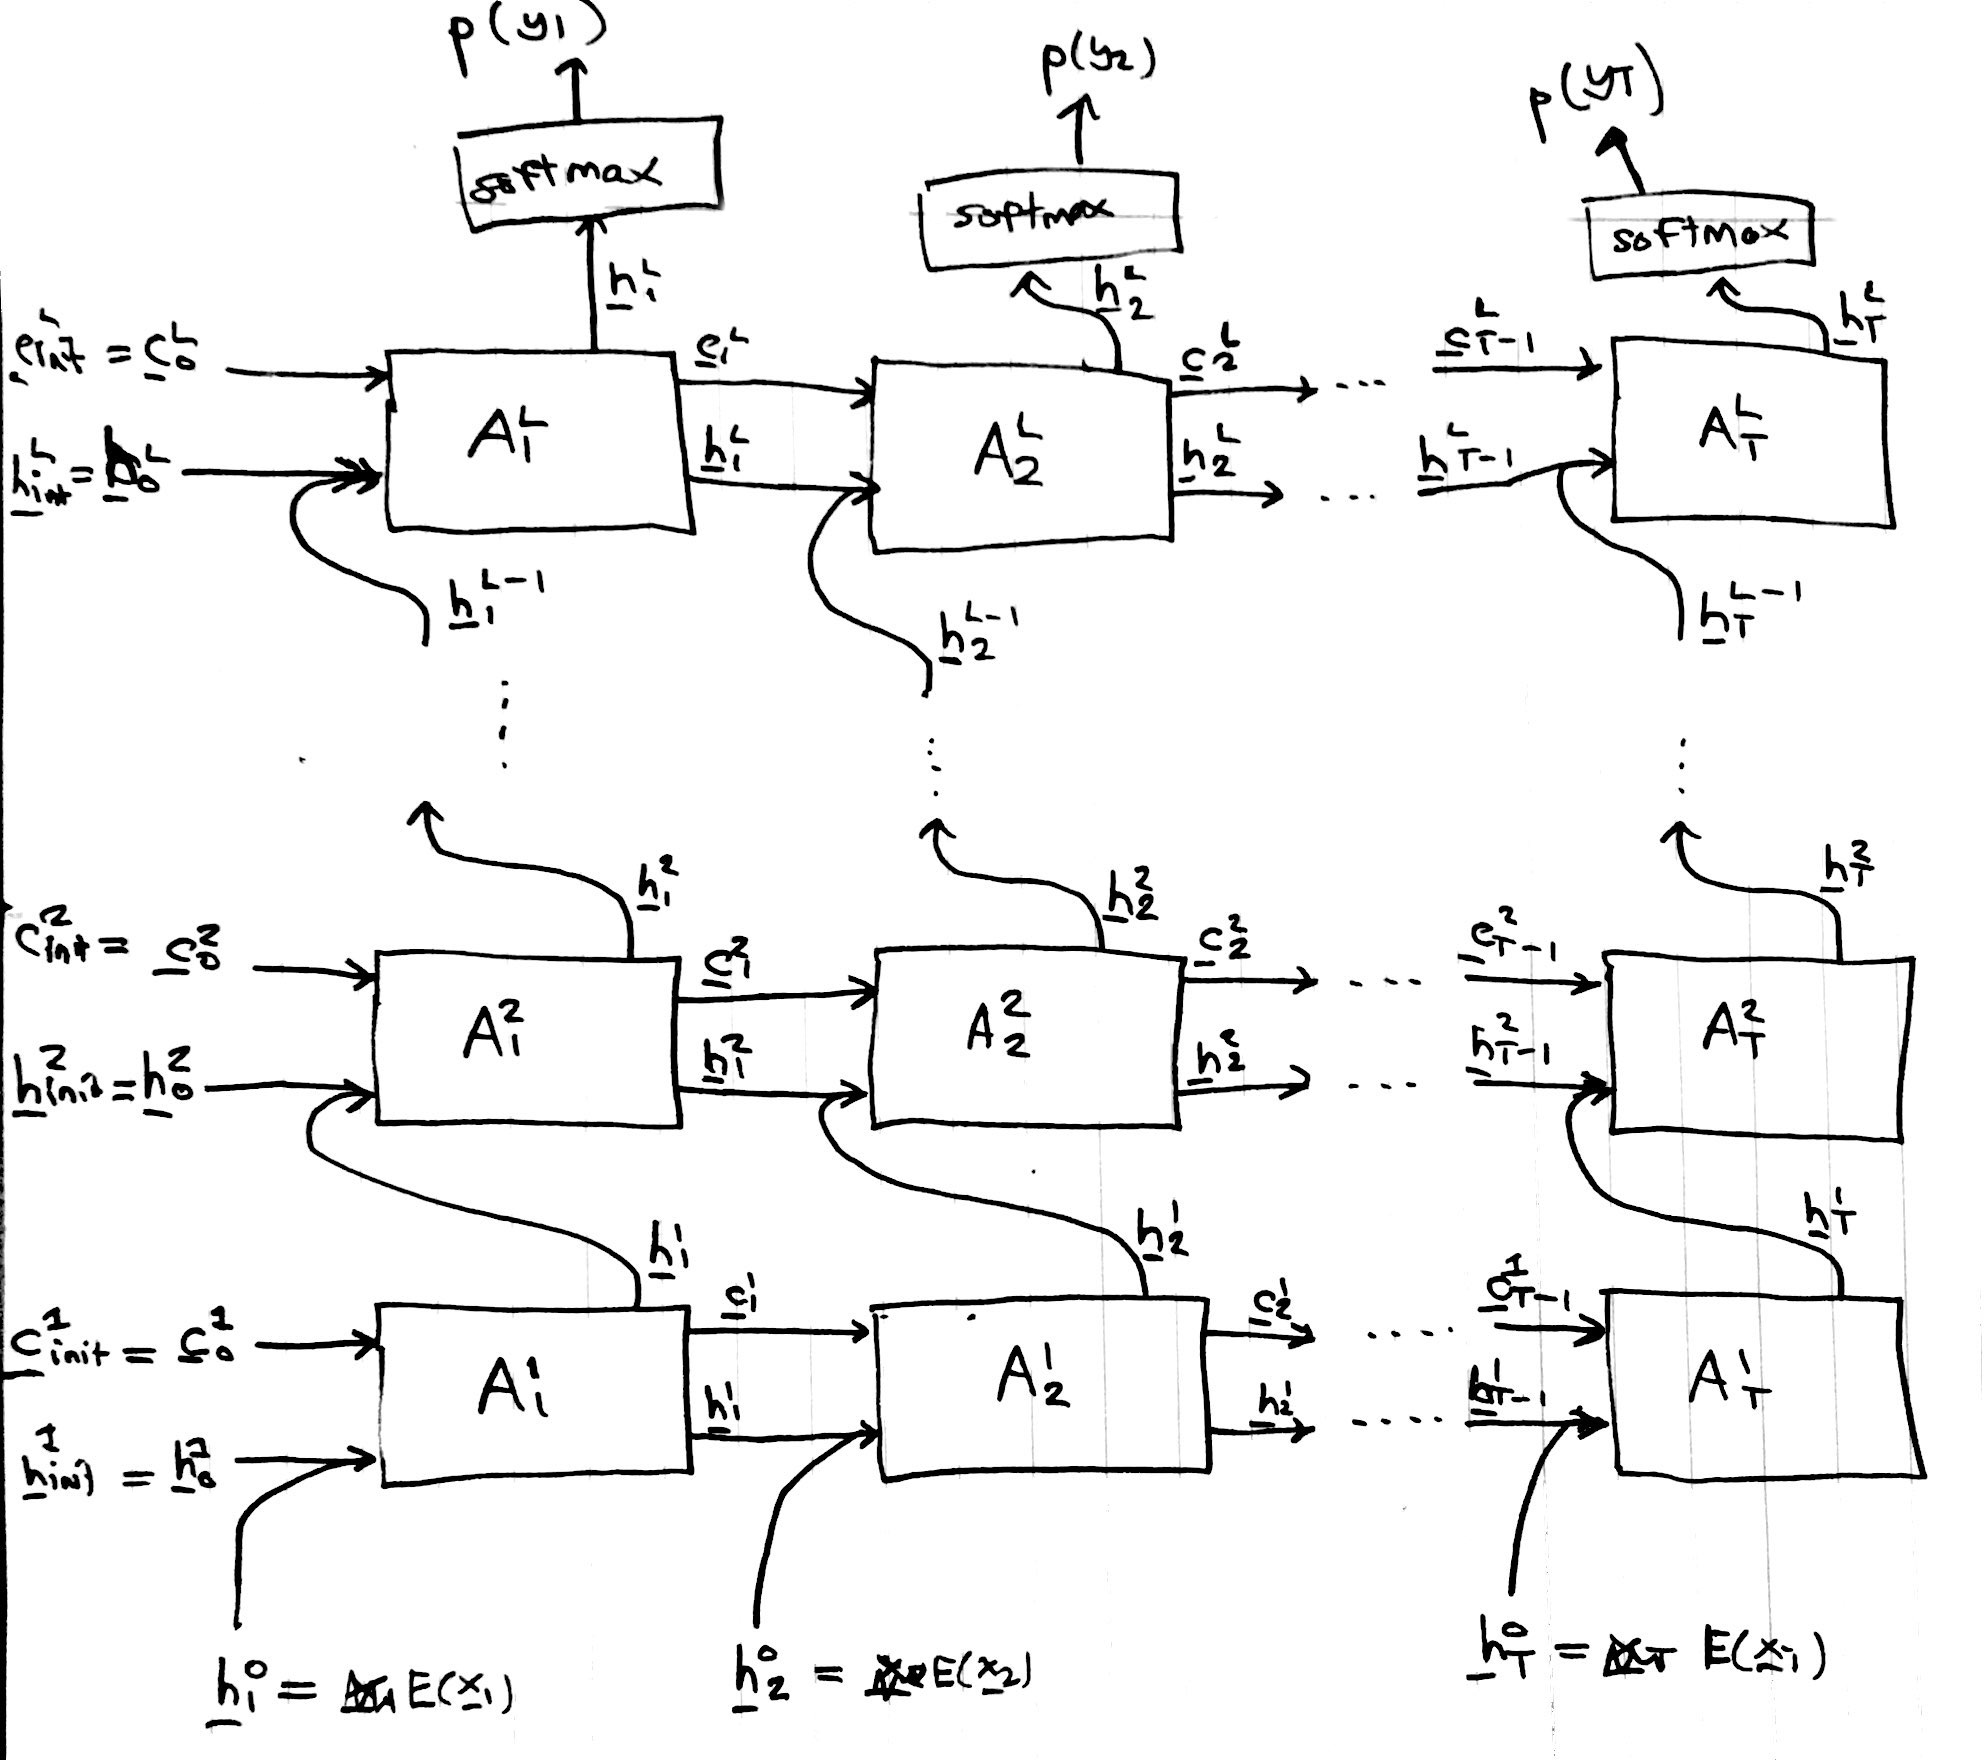
\includegraphics[width=400pt]{figs/lstm_net_tmp.jpg}
\caption{Flow of information in deep LSTM network}
\label{fig:deep-lstm-arch}
\end{figure}

Let $\ast$ denote pointwise vector multiplication. Given input
$\vect{h}_t^{l-1}$, recurrent state $\vect{h}_{t-1}^l$, cell state
$\vect{c}_{t-1}^l$, and writing $\vect{x} = [\vect{h}_{t-1}^l,
\vect{h}_t^{l-1}]$, an LSTM first computes intermediates as per equations
(\ref{eq:lstm-f}) through (\ref{eq:lstm-d}).
\begin{align}
  \vect{f} &= \sigma(\vect{W}_f \vect{x} + \vect{b}_f) \label{eq:lstm-f} \\
  \vect{i} &= \sigma(\vect{W}_i \vect{x} + \vect{b}_i) \\
  \vect{o} &= \sigma(\vect{W}_o \vect{x} + \vect{b}_o) \\
  \vect{d} &= \tanh(\vect{W}_d \vect{x} + \vect{b}_d) \label{eq:lstm-d}
\end{align}
The new states $\vect{c}_t^l$ and $\vect{h}_t^l$ are then computed with
equations (\ref{eq:lstm-c}) and (\ref{eq:lstm-h}). 
\begin{align}
  \vect{c}_t^l &= \vect{f} \ast \vect{c}_{t-1}^l + \vect{i} \ast \vect{d}
  \label{eq:lstm-c} \\
  \vect{h}_t^l &= \vect{o} \ast \tanh(\vect{c}_t^l) \label{eq:lstm-h}
\end{align}

Note that, as before, the parameters are shared across timesteps but not between
layers: layer superscripts are excluded from the parameters in the LSTM
equations for clarity. Figure~\ref{fig:lstm-cell} shows the structure of this
LSTM cell and interprets the LSTM equations graphically.

\begin{figure}[H]
\centering
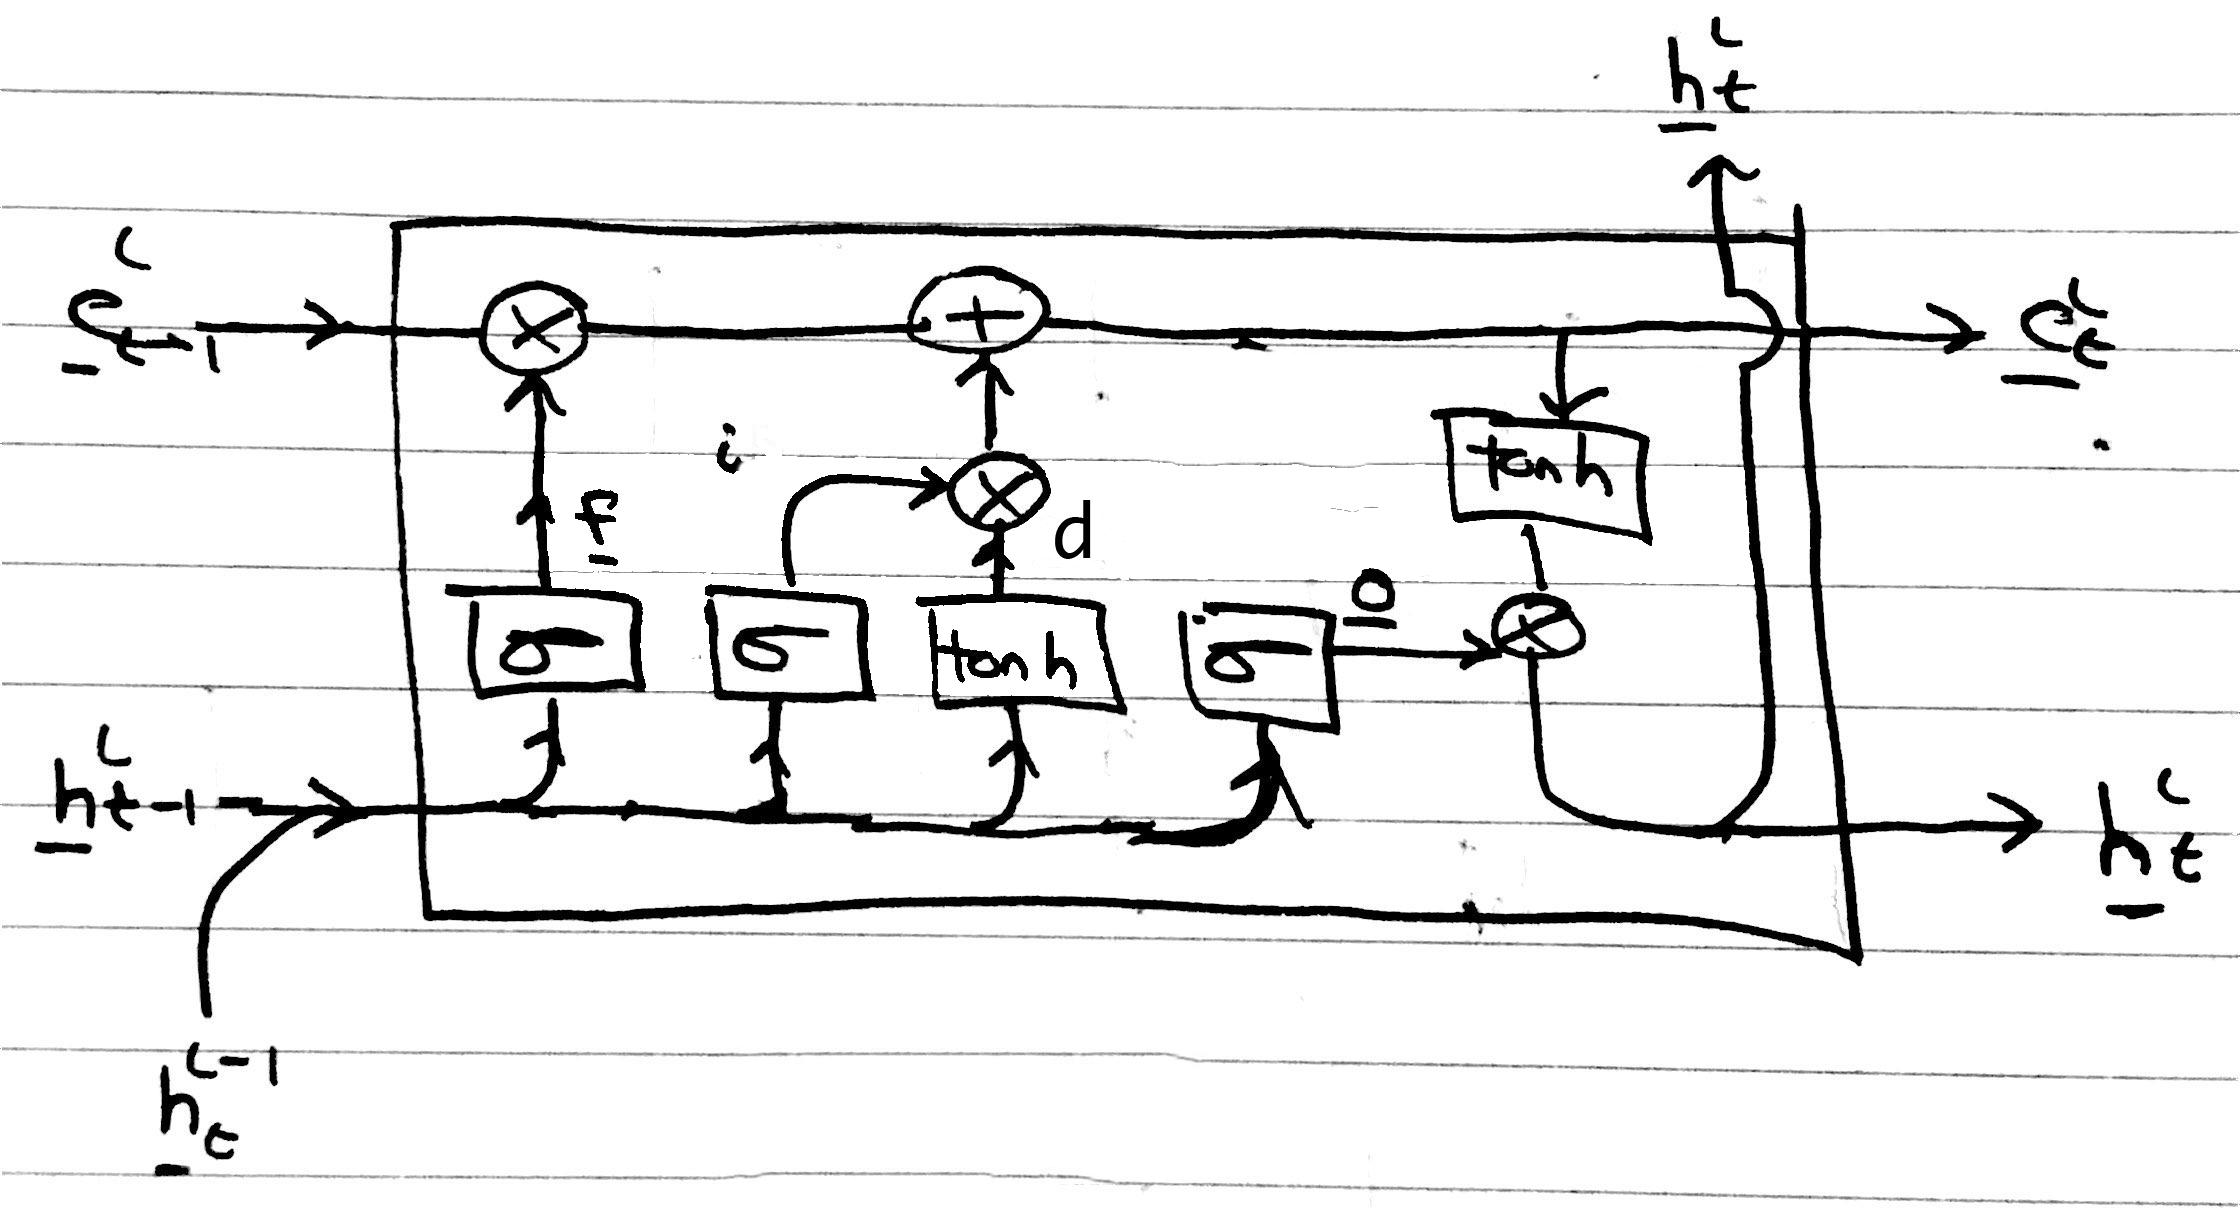
\includegraphics[width=300pt]{figs/lstm_detail_tmp.png}
\caption{LSTM Cell Structure}
\label{fig:lstm-cell}
\end{figure}

\vspace{-2mm}
The purpose of the cell state $\vect{c}_t^l$ is to act as a long-term memory.
The LSTM can be understood intuitively as protecting and using this cell state
by following three principles of selectivity:
\begin{enumerate}[label=\arabic*., itemsep=0mm]
  \item \textbf{Write} selectively: only a summary of the information entering
    the cell should be written to the protected memory.
  \item \textbf{Read} selectively: only a summary of the information stored in
    the cell's memory should be included in the output state vector.
  \item \textbf{Forget} selectively: occasionally, previously-useful memories
    will no longer be relevant, and the cell should forget them.
\end{enumerate}

The sigmoidal units $\vect{f}, \vect{i}$, and $\vect{o}$ are known as the
\emph{gates} of the LSTM cell: they are used to scale the activations of other
units componentwise and regulate the flow of information through the cell. The
function of each of the LSTM units can be understood in terms of these
principles as follows:

\begin{itemize}
  \item $\vect{f}$ is known as the \emph{forget gate}: it selectively removes
    information from the previous cell state.
  \item The tanh layer $\vect{d}$ is known as the \emph{input feature}. It
    computes data that we may wish to store in the protected cell state.
\item $\vect{i}$ is known as the \emph{input gate}: it controls which data from
  the input feature gets written into the cell state.
\item Finally, $\vect{o}$ is the \emph{output gate}: it regulates which data
  gets output based on the cell state.
\end{itemize}

Note that, since the introduction of LSTM, many other variants have appeared.
For example, an LSTM that also considers the previous cell state
$\vect{c}_{t-1}^l$ when evaluating the gate units (equations (\ref{eq:lstm-f})
through (\ref{eq:lstm-d})) is known as an LSTM with \emph{peephole} connections.
Generally, LSTM variants have only been shown to achieve marginal performance
improvements from the standard LSTM architecture (\todo cite!). We shall only
consider the architecture described thus far.

\subsection{Regularisation}

A known problem with neural networks in general is \emph{overfitting}. For deep
feedforward networks, \emph{dropout} \cite{srivastava2014dropout} has seen
significant success in preventing overfitting (regularisation). It was not until
the recent work of Zaremba et al.\ \cite{zaremba2014recurrent} that it was known
how to successfully apply dropout to recurrent networks. The authors determine
that applying dropout to only the non-recurrent connections in the network leads
to successful regularisation. 

\section{Choice of Libraries}

The first significant choice to be made was that of a suitable library to assist
in corpus preparation and musical I/O. Initial inspection of relevant corpora
and their formats indicated that writing a parser for an established music
notation format such as MusicXML would take a considerable amount of time and
offer limited flexibility. After further research, it was decided that the
Python package \texttt{music21}\footnote{http://web.mit.edu/music21/} would be
utilised. \texttt{music21} is an open-source toolkit for computational
musicology. This package was considered ideal for the task of corpus preparation
due to the following features:
\begin{itemize}
  \item Built-in corpora including the Bach chorales in MusicXML format.
  \item Included parser for various music notation formats, including MusicXML.
  \item High-level features for manipulating musical data.
\end{itemize}

The other major choice of library was that of a neural network library to assist
in the implementation of the RNN. I was specifically looking for a library where
the level of abstraction is such that there is considerable flexibility provided
to the user, but mundane tasks such as calculating the gradients to perform the
backwards pass through the network during training were handled by the library.

Google's TensorFlow \cite{abadi2016tensorflow}, with its primary abstraction
being the \emph{computational graph}, was considered the ideal tool for this
purpose.  Furthermore, TensorFlow was considered advantageous due to
its very large user base, and therefore increased availability of information
and support concerning the library.

\section{Software Engineering Methodology}

I decided to adopt an \emph{agile} development methodology when undertaking the
implementation. Agile was chosen primarily for the flexibility offered in the
face of changing timescales and requirements.

\todo Timeline/Gantt chart.

\chapter{Implementation}\label{chap:impl}

\section{Corpus Preparation and Analysis}\label{sec:corpus-prep-analysis}

Before beginning the implementation of either model, the corpus needed to be
processed and exported to a common format. The high-level description of the
chosen corpus representation in Section~\ref{sec:corp-rep} was made concrete by
using a JSON format to encode the chorales. JSON was chosen due to the
readily-available library support in both Python and \texttt{C++}, as well as
the human-readable nature of the format, so as to simplify the debugging
process. This JSON format was later used not only for the corpus, but also for
musical I/O of both models.

\vspace{4mm}
\begin{minted}[frame=single, linenos=true, fontsize=\footnotesize]{js}
{
  "title": "Aus meines Herzens Grunde (Excerpt)",
  "bwv": "269",
  "time_sig_amt": 12,
  "key_sig_sharps": 1,
  "notes": [
    [67, 8,  4], [67, 12, 8], [74, 20, 4], [71, 24, 6], 
    [69, 30, 2], [67, 32, 4], [67, 36, 6], [69, 42, 2], 
    [71, 44, 4], [69, 48, 8], [71, 56, 4], [74, 60, 8], 
    [72, 68, 4], [71, 72, 4], [69, 76, 8], [67, 84, 8]
  ]
}
\end{minted}

\begin{figure}[H]
\centering
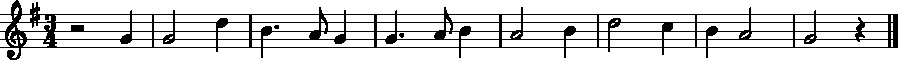
\includegraphics[width=450pt]{figs/aus_meines_excerpt.pdf}
\caption{JSON Chorale excerpt with corresponding score}
\label{fig:chorale-excerpt}
\end{figure}

An example encoding of a chorale melody using this JSON representation is given
in Figure~\ref{fig:chorale-excerpt}. 

Tonality metadata was extracted in the form of key signatures represented as
integers in $[-7,7]$, where a positive number indicates the number of sharps,
and a negative number the number of flats.  Time signatures are represented as
the number of semiquavers in a bar, which suffices to distinguish
\lilyTimeSignature{3}{4} and \lilyTimeSignature{4}{4}, the two time signatures
used in the chorales.

Alternative representations such as a list of accidentals to represent a key
signature, or an exact representation of the time signature were considered.
However, these representations are relatively wasteful in space, and are
\emph{sparse} with respect to the corpus. Dense representations such as those
chosen are preferred in the literature, and are more suitable in conjunction
with our representation of musical types in \texttt{C++} (see
Section~\ref{sec:cpp-event-rep}).

\begin{figure}[H]
\centering
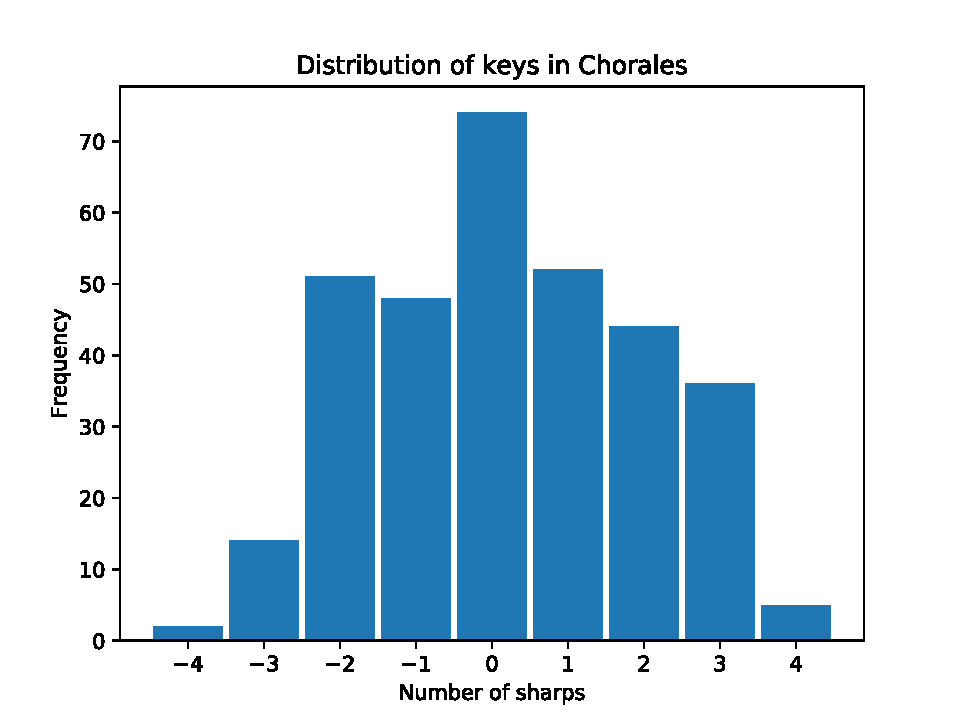
\includegraphics[width=300pt]{figs/key_dist.pdf}
\caption{Histogram showing distribution of key signatures in corpus}
\label{fig:key-dist}
\end{figure}

\begin{figure}[H]
\centering
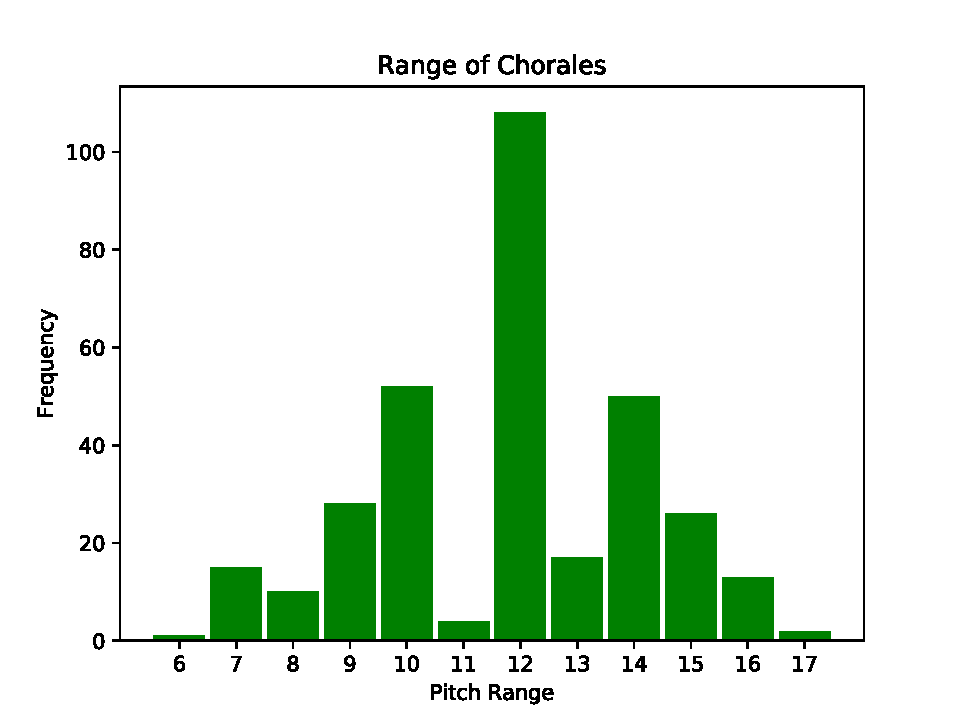
\includegraphics[width=300pt]{figs/range_dist.pdf}
\caption{Histogram showing distribution of pitch range in chorales}
\label{fig:range-dist}
\end{figure}

In addition to extracting the melodies from the \texttt{music21} chorale corpus
and encoding them in our JSON format, the corpus preparation script performs
some analysis on the corpus to determine the syntactic domains of the various
types of interest in our corpus. That is, the script computes the set of
pitches, durations, intervals, etc.\ that occur in the chorales, and stores
these as metadata along with the corpus. This informed the construction of
\texttt{C++} classes to represent these musical types (see
Section~\ref{sec:cpp-event-rep}). Figures~\ref{fig:key-dist} and
\ref{fig:range-dist} exemplify the analysis performed on the corpus.

The source corpus, packaged in \texttt{music21}, consists of MusicXML files
describing notation for Bach's four-part chorale harmonisations. During the
corpus preparation process, I use \texttt{music21} to parse these XML files,
extract the soprano part, and output the data in the established JSON format, as
well as performing additional processing such as \emph{anacrusis} (pick-up)
detection. By preprocessing the corpus, we factor out this process from the
point at which data is ingested into each model.

\section{Multiple Viewpoint System}

\subsection{Overview}

\begin{figure}[H]
\centering
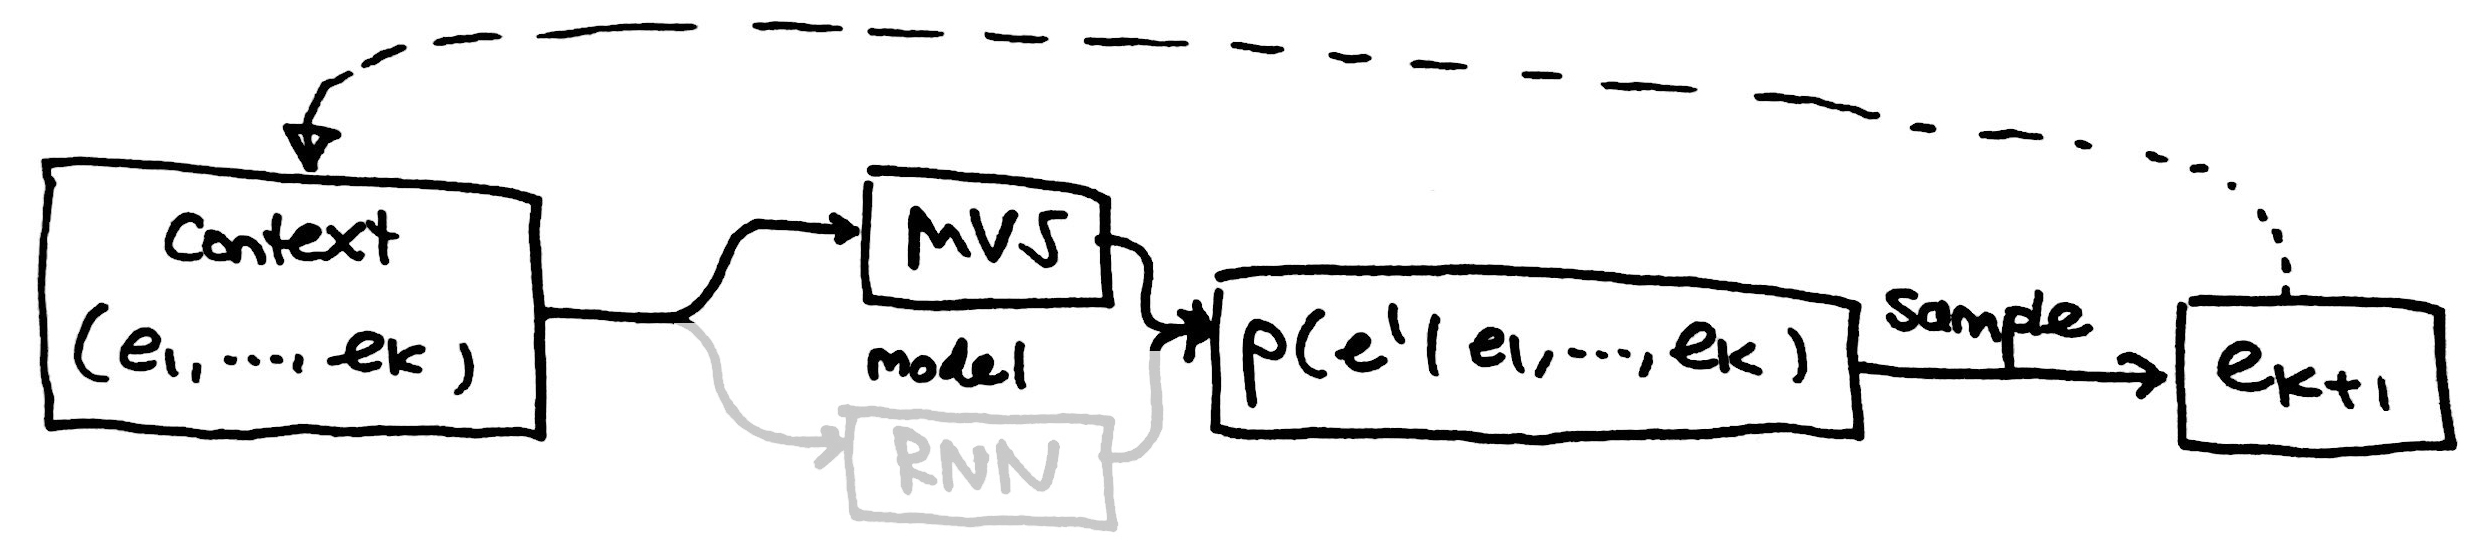
\includegraphics[width=400pt]{figs/high_level_mvs_tmp.jpg}
\caption{Overview of music generation using MVS}
\label{fig:mvs-gen-overview}
\end{figure}

A complete framework for implementing Multiple Viewpoint Systems in \verb!C++!
has been implemented and released as an open source project for others to use.
Since no existing framework was available, this had to be implemented from
scratch. The framework implements the formalism detailed in
Section~\ref{sec:mvs-formalism} in full. I chose to make the implementation as
general as possible so that it may be of use in other contexts in the future. 

This general framework was then specialised to the task of chorale melody
generation. At the core of the framework, the \emph{prediction by partial match}
(PPM) algorithm was implemented for smoothing variable-order context models. The
distributions predicted by these context models are combined using the
entropy-weighted schemes described in Section~\ref{sec:vp-comb}.

Template-based abstractions were made such that, using these primitives, \emph{basic},
\emph{derived}, \emph{linked}, and \emph{triply-linked} viewpoints can be
instantiated over arbitrary combinations of types. Both a \emph{long-term}
model, for capturing regularity throughout the corpus, and a \emph{short-term}
model, for capturing the regularity within a composition, were implemented.
Sampling by iterative random walk was implemented for melody generation.
Finally, an automatic viewpoint selection algorithm in the form of \emph{forward
step-wise selection} \cite{pearce2005construction} was implemented.

\begin{figure}[H]
\centering
  \trimbox{0cm 2.5cm 0cm 0cm}{ 
  \begin{tikzpicture}
  \umlclass[type=interface, template={$\zeta$,
    $T_{\text{predict}}$}]{Predictor}{}{
    +predict(context : $\zeta^*$) : dist$\langle T_{\text{predict}}
    \rangle$  \\
    +learn(sequence : $\zeta^*$)
  }
  \umlsimpleclass[y=-4, template={$\zeta$, $T_{\text{viewpoint}}$}]{GeneralViewpoint}
  \umlsimpleclass[x=9, template={$\zeta$, $T_l$, $T_r$}]{GeneralLinkedVP}

  \umlsimpleclass[x=9,y=-4, alias=seqspeclink]{SequenceModel}
  \umlsimpleclass[y=-7, alias=seqspec]{SequenceModel}
  \umlsimpleclass[y=-7,x=9, template={$T$}, alias=seqgen]{SequenceModel}
  \umlsimpleclass[y=-10,x=9, alias=ctxspec]{ContextModel}
  \umlsimpleclass[y=-10, alias=ctxgen, template={$b$}]{ContextModel}
  \umlsimpleclass[y=-13]{TrieNode}
  
  \umlimpl{GeneralViewpoint}{Predictor}
  \umlimpl{GeneralLinkedVP}{Predictor}

  \umlunicompo[arg=model, mult=1]{GeneralViewpoint}{seqspec}
  \umlunicompo[arg=model, mult=1]{GeneralLinkedVP}{seqspeclink}
  \umlreal[stereo={$T \rightarrow T_{\text{viewpoint}}$}]{seqspec}{seqgen}
  \umlreal[stereo={$T \rightarrow \text{Pair}\langle T_l, T_r
  \rangle$}]{seqspeclink}{seqgen}
  
  \umlunicompo[arg=model, mult=1]{seqgen}{ctxspec}
  \umlreal[stereo={$b \rightarrow T::\text{cardinality}$}]{ctxspec}{ctxgen}

  \umlunicompo[arg=trie root, mult=1]{ctxgen}{TrieNode}
  \umlunicompo[arg=children, mult=0..b, recursive=-90|2|3cm]{TrieNode}{TrieNode}
\end{tikzpicture}
}
\hspace{-10mm}
\caption{UML Class Diagram of Prediction Stack}
\label{fig:uml-prediction}
\end{figure}

The principal design strategy of the implementation was to achieve a symmetry
and tight correspondence between the \texttt{C++} type system and the formalism
of multiple viewpoints detailed in Section~\ref{sec:mvs-formalism}. This was
considered desirable for a number of reasons:
\begin{itemize}
  \item A correspondence between the \texttt{C++} type system and the MVS
    formalism provides the basis for a clean API that should be easily
    understood by both \texttt{C++} programmers and those familiar with the
    formalism.
  \item Making full use of the type system in a statically-typed language can
    ensure that many more potential programmer errors are caught at compile time
    than otherwise would be.
\end{itemize}

\texttt{C++} templates were considered the ideal tool to achieve this. Templates
are \emph{flexible}, allow for considerable \emph{generality}, and are evaluated
at compile time, achieving better safety guarantees: in particular, they can
eliminate much of the need for dynamic memory allocation, a cause of many common
runtime issues. As we shall see, specific viewpoints can be implemented by
specialising the template classes \texttt{GeneralViewpoint} and
\texttt{GeneralLinkedVP}. 

Despite templates being the primary means of achieving polymorphism, inheritance
polymorphism is used to implement an abstract base class for viewpoints (see
Figure~\ref{fig:uml-prediction}). This was done in order to unify the
otherwise-heterogeneous viewpoint types predicting a particular basic type. For
example, viewpoints $\emph{duration} \otimes \emph{pitch}$, \emph{seqint}, and
\emph{pitch} have different corresponding types, but are all predictors of
pitch: we want to refer to them polymorphically as such.

We shall now give a brief overview of the main components implemented to gain an
appreciation of the intent behind each component and how the overall system fits
together before taking a closer look at various parts of the implementation.

\begin{itemize}
  \item \texttt{TrieNode<b>} is a generic implementation of the trie data
    structure with branching factor \texttt{b}. Specifying the branching factor
    at compile time allows the space-efficient implementation of tries over
    types $\tau$ with varying cardinality $|[\tau]|$.
  \item Using this trie implementation, \texttt{ContextModel<b>} implements a
    context model over an alphabet of size \texttt{b}, as per
    Section~\ref{sec:ctx-model-prep}. The inference algorithm is PPM A with
    exclusion.
  \item A simple, unified representation for domain-specific types is used
    throughout.  These are passed as template parameters to many different
    classes. Examples include basic types such as \texttt{ChoralePitch} and
    \texttt{ChoraleDuration}, derived types such as \texttt{ChoraleInterval} and
    abstract meta-types such as \texttt{EventPair<T1,T2>}.
  \item \texttt{SequenceModel<T>} further abstracts \texttt{ContextModel} by
    implementing a higher-level interface to context models in terms of these
    domain-specific types.
  \item \texttt{EventDistribution<T>} represents a probability distribution over
    a type \texttt{T}. It supports random sampling as well as multiple
    distribution combination schemes as per Section~\ref{sec:vp-comb}. Objects
    of this type are returned by \texttt{SequenceModel} objects when predicting
    the next event in a sequence.
  \item All viewpoint implementations derive from the
    \texttt{Predictor<EventSpace,T>} template interface. These are outlined in
    Figure~\ref{fig:uml-prediction} but also include a triply-linked viewpoint
    implementation. Such objects contain an underlying \texttt{SequenceModel}
    object and support the operations of \emph{lifting} and \emph{reification}
    as per Section~\ref{sec:mvs-formalism}.
  \item \texttt{ChoraleVPLayer} is a container for multiple viewpoints over
    the chorale-specific types, used to
    implement both the \emph{long-term} and \emph{short-term} model.
  \item Finally, \texttt{ChoraleMVS} is a high-level class which manages all the
    components of a multiple viewpoint system over chorales and provides a
    unified interface for tasks such as \emph{prediction} and \emph{generation}.
    Figure~\ref{fig:chorale-uml} illustrates how these components relate to each
    other.
\end{itemize}

\begin{figure}[H]
\centering
  \trimbox{0cm 0.0cm 0cm 0cm}{ 
  \begin{tikzpicture}
  
  \umlclass{ChoraleMVS}{
    - short\_term\_layer : ChoraleVPLayer \\
    - long\_term\_layer : ChoraleVPLayer
  }{
    + add\_viewpoint$\langle T \rangle$(vp : ChoralePredictor$\langle T\rangle$ *) \\
    + predict$\langle T\rangle$(context : vec$\langle$ChoraleEvent$\rangle$) :
    dist$\langle T \rangle$ \\
    + cross\_entropy(seq : vec$\langle$ChoraleEvent$\rangle$) : double \\
    + generate(length : int, ts : TimeSig) : vec$\langle$ChoraleEvent$\rangle$
    \\
    + learn(example : vec$\langle$ChoraleEvent$\rangle$)
  }
  \umlsimpleclass[y=-5]{ChoraleVPLayer}
  \umlsimpleclass[x=-5, y = -9, alias=pitchpred]{Predictor}
  \umlsimpleclass[x=0, y = -9, alias=durpred]{Predictor}
  \umlsimpleclass[x=5, y = -9, alias=restpred]{Predictor}
  \umlsimpleclass[y = -13, type=interface, template={$T$}, alias=cpred]{Predictor}
  \umlsimpleclass[y = -17, type=interface, template={$\zeta$, $T$},
alias=predbase]{Predictor}
  
  \umlunicompo[arg=short-term, mult=1, anchors=-115 and 160]{ChoraleMVS}{ChoraleVPLayer} 
  \umlunicompo[arg=long-term, mult=1, anchors=-65 and 20]{ChoraleMVS}{ChoraleVPLayer}
  \umluniaggreg[arg=pitch\_vps, mult=1..*]{ChoraleVPLayer}{pitchpred}
  \umluniaggreg[arg=duration\_vps, mult=1..*]{ChoraleVPLayer}{durpred}
  \umluniaggreg[arg=rest\_vps, mult=1..*]{ChoraleVPLayer}{restpred}
  \umlreal[stereo={$T \rightarrow$ ChoralePitch}, pos stereo=0.3]{pitchpred}{cpred}
  \umlreal[stereo={$T \rightarrow$ ChoraleDuration}, pos stereo=0.55]{durpred}{cpred}
  \umlreal[stereo={$T \rightarrow$ ChoraleRest}, pos stereo=0.3]{restpred}{cpred}
  \umlreal[stereo={$\zeta \rightarrow$ ChoraleEvent}]{cpred}{predbase}
\end{tikzpicture}
}
\hspace{-10mm}
\caption{UML Class Diagram relating viewpoint framework with Chorale
hierarchy}
\label{fig:chorale-uml}
\end{figure}

\subsection{Context Models}

Recall from Section~\ref{sec:ctx-model-prep} that a context model populates a
database of examples during training and subsequently uses an inference
procedure to perform contextual prediction by matching the context against the
database. We first tackle the task of constructing the underlying data
structure, and then turn to the implementation of PPM.

Given an example sequence $e_1^k$, we need to extract all $h$-grams from this
sequence in order to populate the trie data structure. The procedure for this
can be thought of as passing a sliding window over the input sequence and
generating subsequences. This procedure is detailed in
Algorithm~\ref{alg:sliding-window} and illustrated in
Figure~\ref{fig:hgram-extract} for an input sequence $e_1^5$.

\vspace{4mm}

\begin{algorithm}[H]
  \caption{Sliding window algorithm for $h$-gram extraction}
  \label{alg:sliding-window}
  \begin{algorithmic}[1]
    \Function{learn-sequence}{$e_1^k \in [\tau]^*$}
      \For{$j : 1 \rightarrow k$}
      \Comment $j$: window end position
        \State \Call{add-or-increment}{()}
        \For{$i : \min(1,j - \hbar + 1) \rightarrow j$} 
        \Comment $i$: window start position
          \State \Call{add-or-increment}{$e_i^j$}
        \EndFor
      \EndFor
    \EndFunction
  \end{algorithmic}
\end{algorithm}

\begin{figure}[H]
\centering
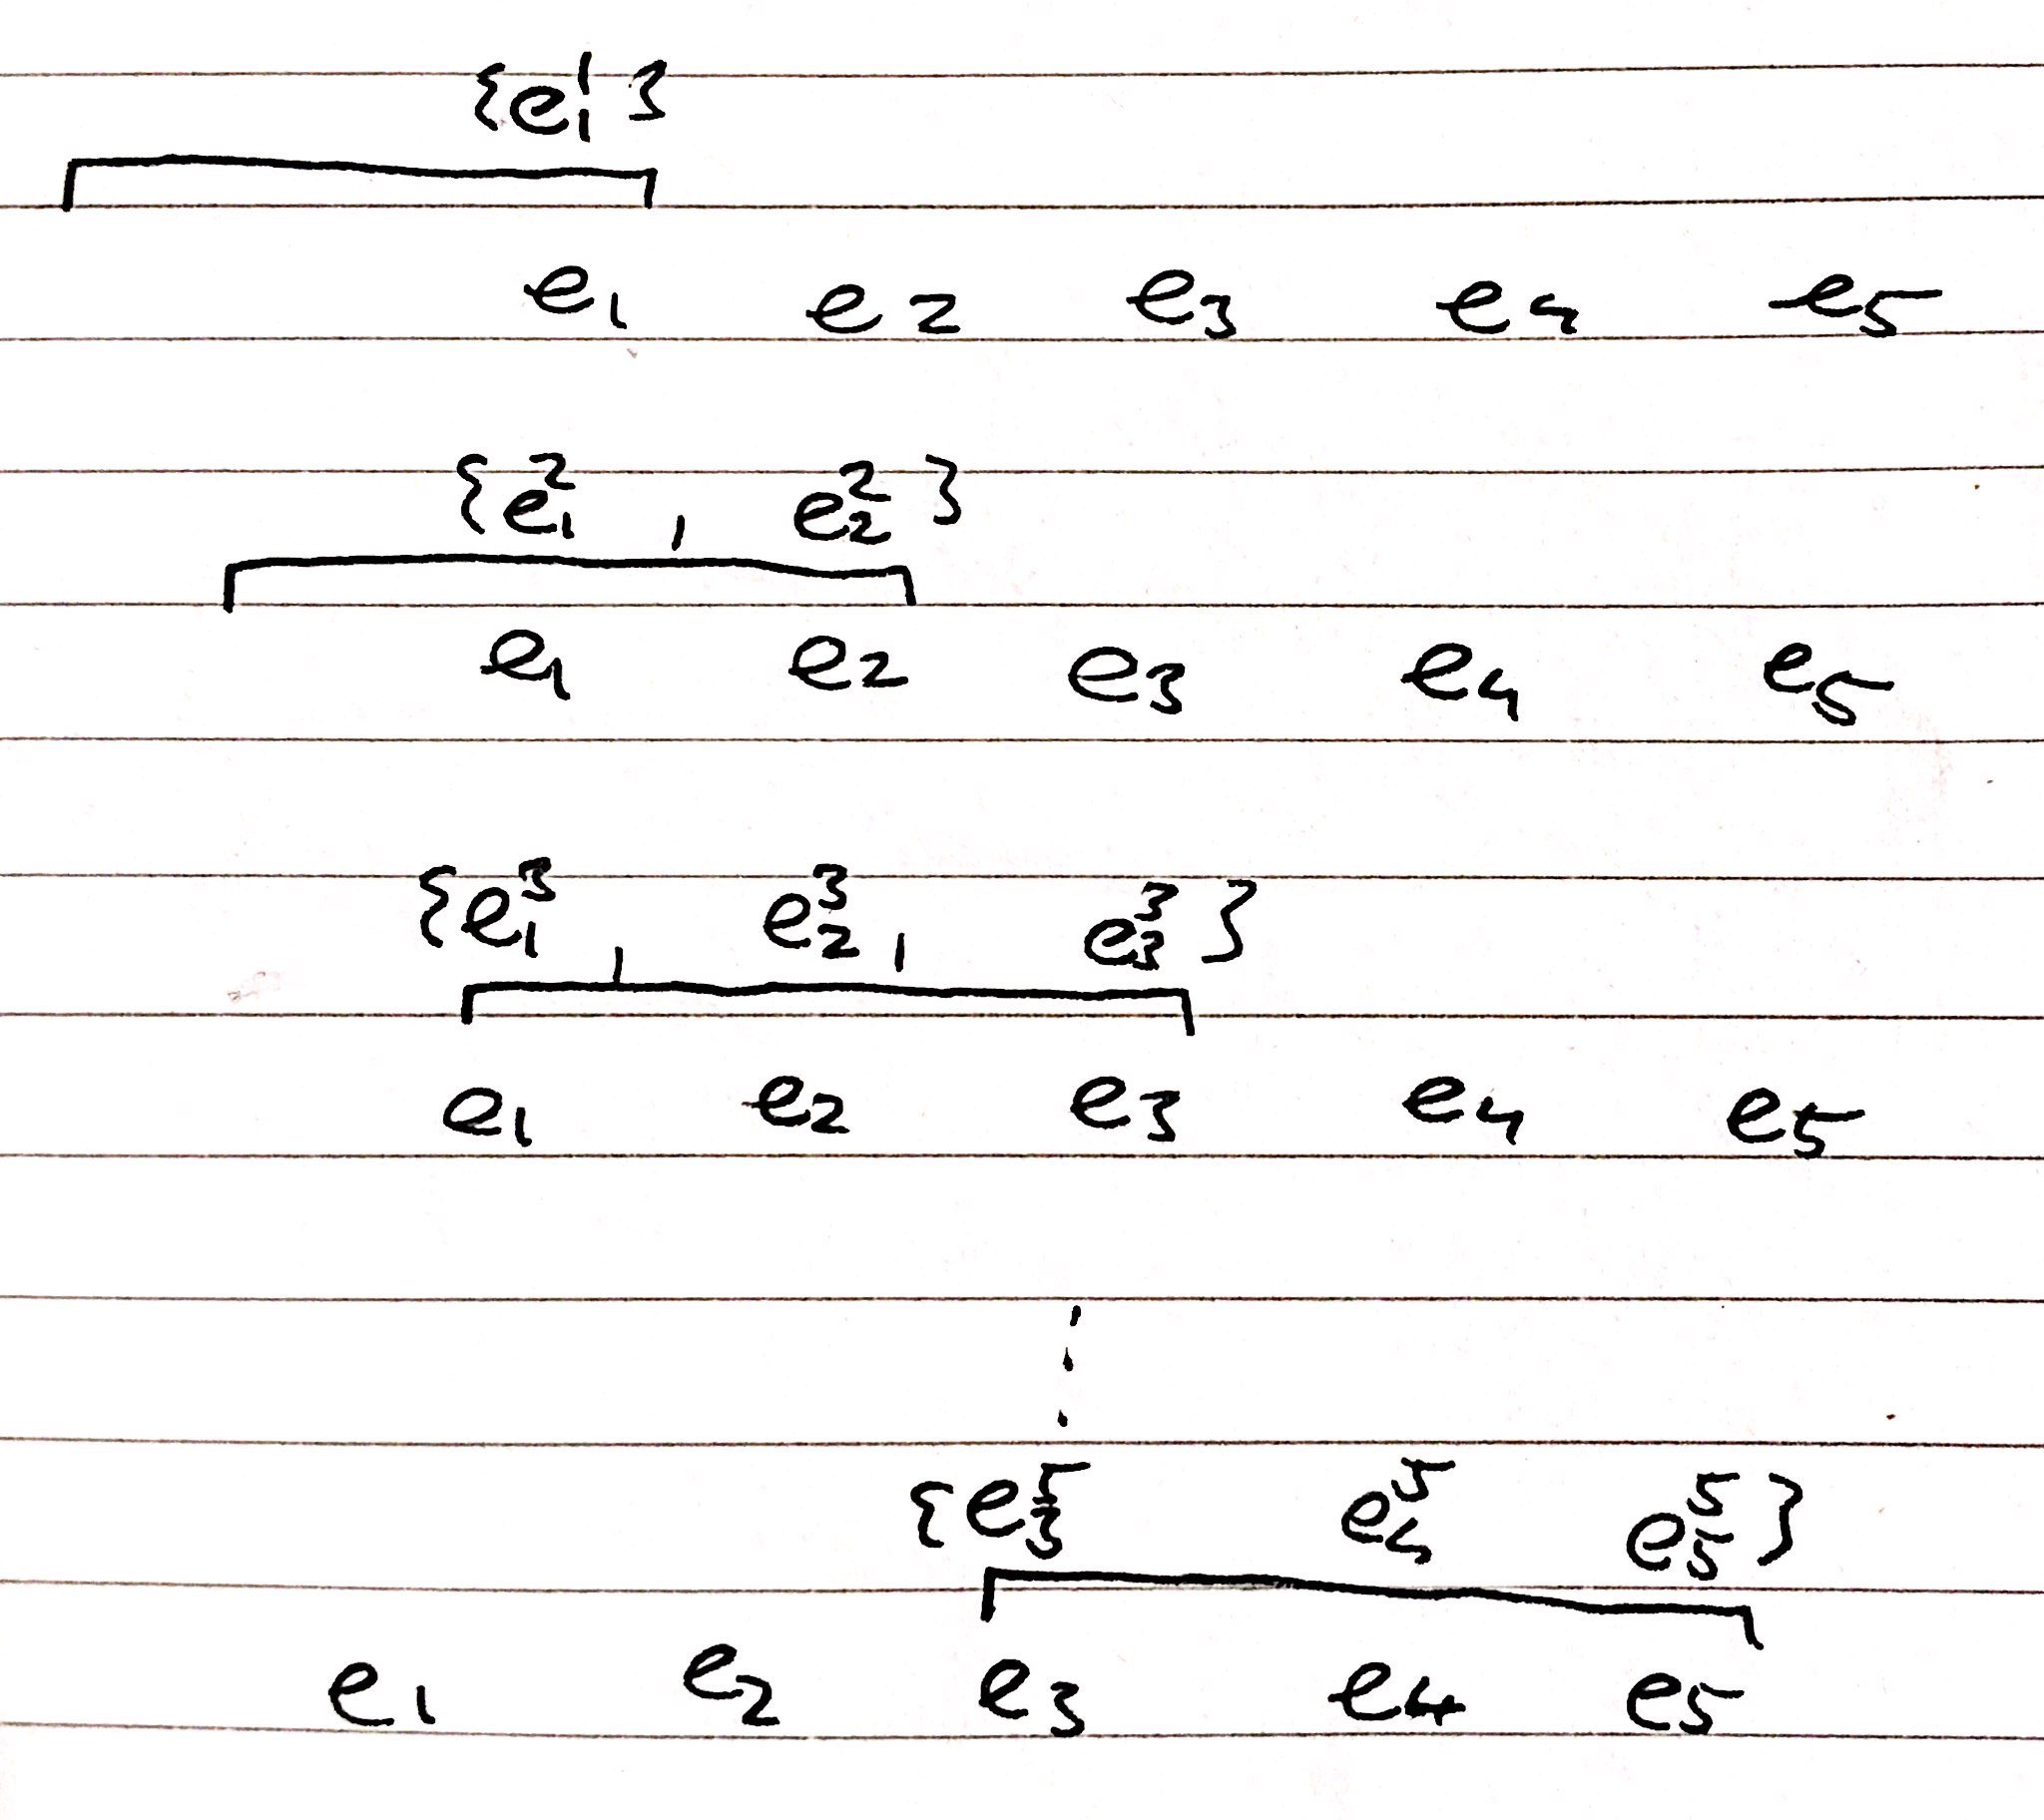
\includegraphics[width=250pt]{figs/sliding_window_tmp.jpg}
\caption{Illustration of the $h$-gram extraction algorithm with $\hbar = 3$}
\label{fig:hgram-extract}
\end{figure}

The function \Call{add-or-increment}{$e_i^j$} looks up $e_i^j$ in the trie. If
it is found, then its count is incremented. Otherwise, $e_i^j$ is inserted into
the trie, the resulting node initialised with a count of unity. Note that $()$,
the empty sequence, corresponds to the root node in the trie.

While this algorithm can be used to construct a long-term model, a short-term
model requires a context model that can be updated online during sequence
prediction. Therefore, context models also need to implement a method which just
extracts those $h$-grams at the tail of the sequence (with the window at the far
right).

\subsubsection{Implementing PPM}

Recall from the discussion in Section~\ref{sec:ctx-model-prep} that considerable
care must be taken to ensure the normalisation of the distributions predicted by
PPM. The technique of \emph{exclusion} maintains state during the trie traversal
in order to reason about the possible context matches at each stage of
execution. Algorithm~\ref{alg:ppm-a} details pseudocode for PPM A with exclusion
which was derived from the high-level descriptions given in the literature.

The key to exclusion in this algorithm is the \textit{Dead} set that
is maintained throughout the recursion. This set should be initialised to
$\varnothing$ and later populated with those events that we \emph{could} have
already matched at a higher-order model and therefore no longer need to consider
at lower-order models. To compute $\mathbb{P}(e' | e_1^k)$ we call
\Call{ppm-a}{$e_1^k$, $e'$, $1$, $\varnothing$}.

\begin{algorithm}[H]
  \caption{PPM A with exclusion}
  \label{alg:ppm-a}
  \begin{algorithmic}[1]
    \Function{ppm-a}{$e_1^k \in [\tau]^*$, $e' \in [\tau]$, $i_{\mathrm{begin}}$, 
    $\textit{Dead} \subseteq [\tau]$}
      \State $\textit{Alive} \gets [\tau] \setminus \textit{Dead}$
      \If{$i_{\mathrm{begin}} > k$}
      \State \Return $1 / |\textit{Alive}|$ \Comment{Base case: uniform
      distribution}
      \EndIf
      \State $i \gets i_{\mathrm{begin}}$
      \For{$i : i_{\mathrm{begin}} \rightarrow k$}
      \If{$C(e_i^k) > 0$} \textbf{break}
      \Comment{Find longest context match}
        \EndIf       
      \EndFor 
      \State $\textit{Known} \gets \set{ e'' \in [\tau]\ |\ C(e_i^k :: e'') > 0 }$
      \State $\textit{Novel} \gets Alive \setminus Known$ \Comment{All
      events we could escape for}
      \State $s \gets \sum_{e'' \in \textit{Alive}} C(e_i^k :: e'')$ 
      \If{$\textit{Novel} = \varnothing$}
        \State \Return $C(e_i^k :: e') / s$ \Comment{No possible need for escape}
      \EndIf
      \If{$e' \in \textit{Known}$}
      \State \Return $C(e_i^k::e') / (1 + s)$ \Comment{Matched $e_i^k::e'$}
      \EndIf
      \State \Return \Call{ppm-a}{$e_1^k$, $e'$, $i+1$, $Dead \cup Known$}$ / (1
      + s)$ \Comment{Escape recursively}
    \EndFunction
  \end{algorithmic}
\end{algorithm}

To realise this pseudocode in \texttt{C++}, the PPM implementation in a
\texttt{ContextModel<b>} instance (with alphabet size \texttt{b}) utilises
bitvectors implemented using \texttt{std::bitset<b>} to efficiently represent
sets of nodes. This achieves better efficiency than alternatives such as
\texttt{std::array<b, bool>} in both space and time: typical implementations
pack bits into machine words and implement the bitwise operations directly.

Figure~\ref{fig:ppm-stepwise} shows the step-by-step execution of this algorithm
computing $\mathbb{P}(\beta|\alpha\gamma)$ on a context model over the alphabet $\Sigma =
\set{\alpha,\beta,\gamma,\delta}$ having seen the training sequence
$(\alpha,\beta,\gamma,\delta,\alpha,\gamma,\alpha,\delta)$.

\begin{figure}[H]
\centering
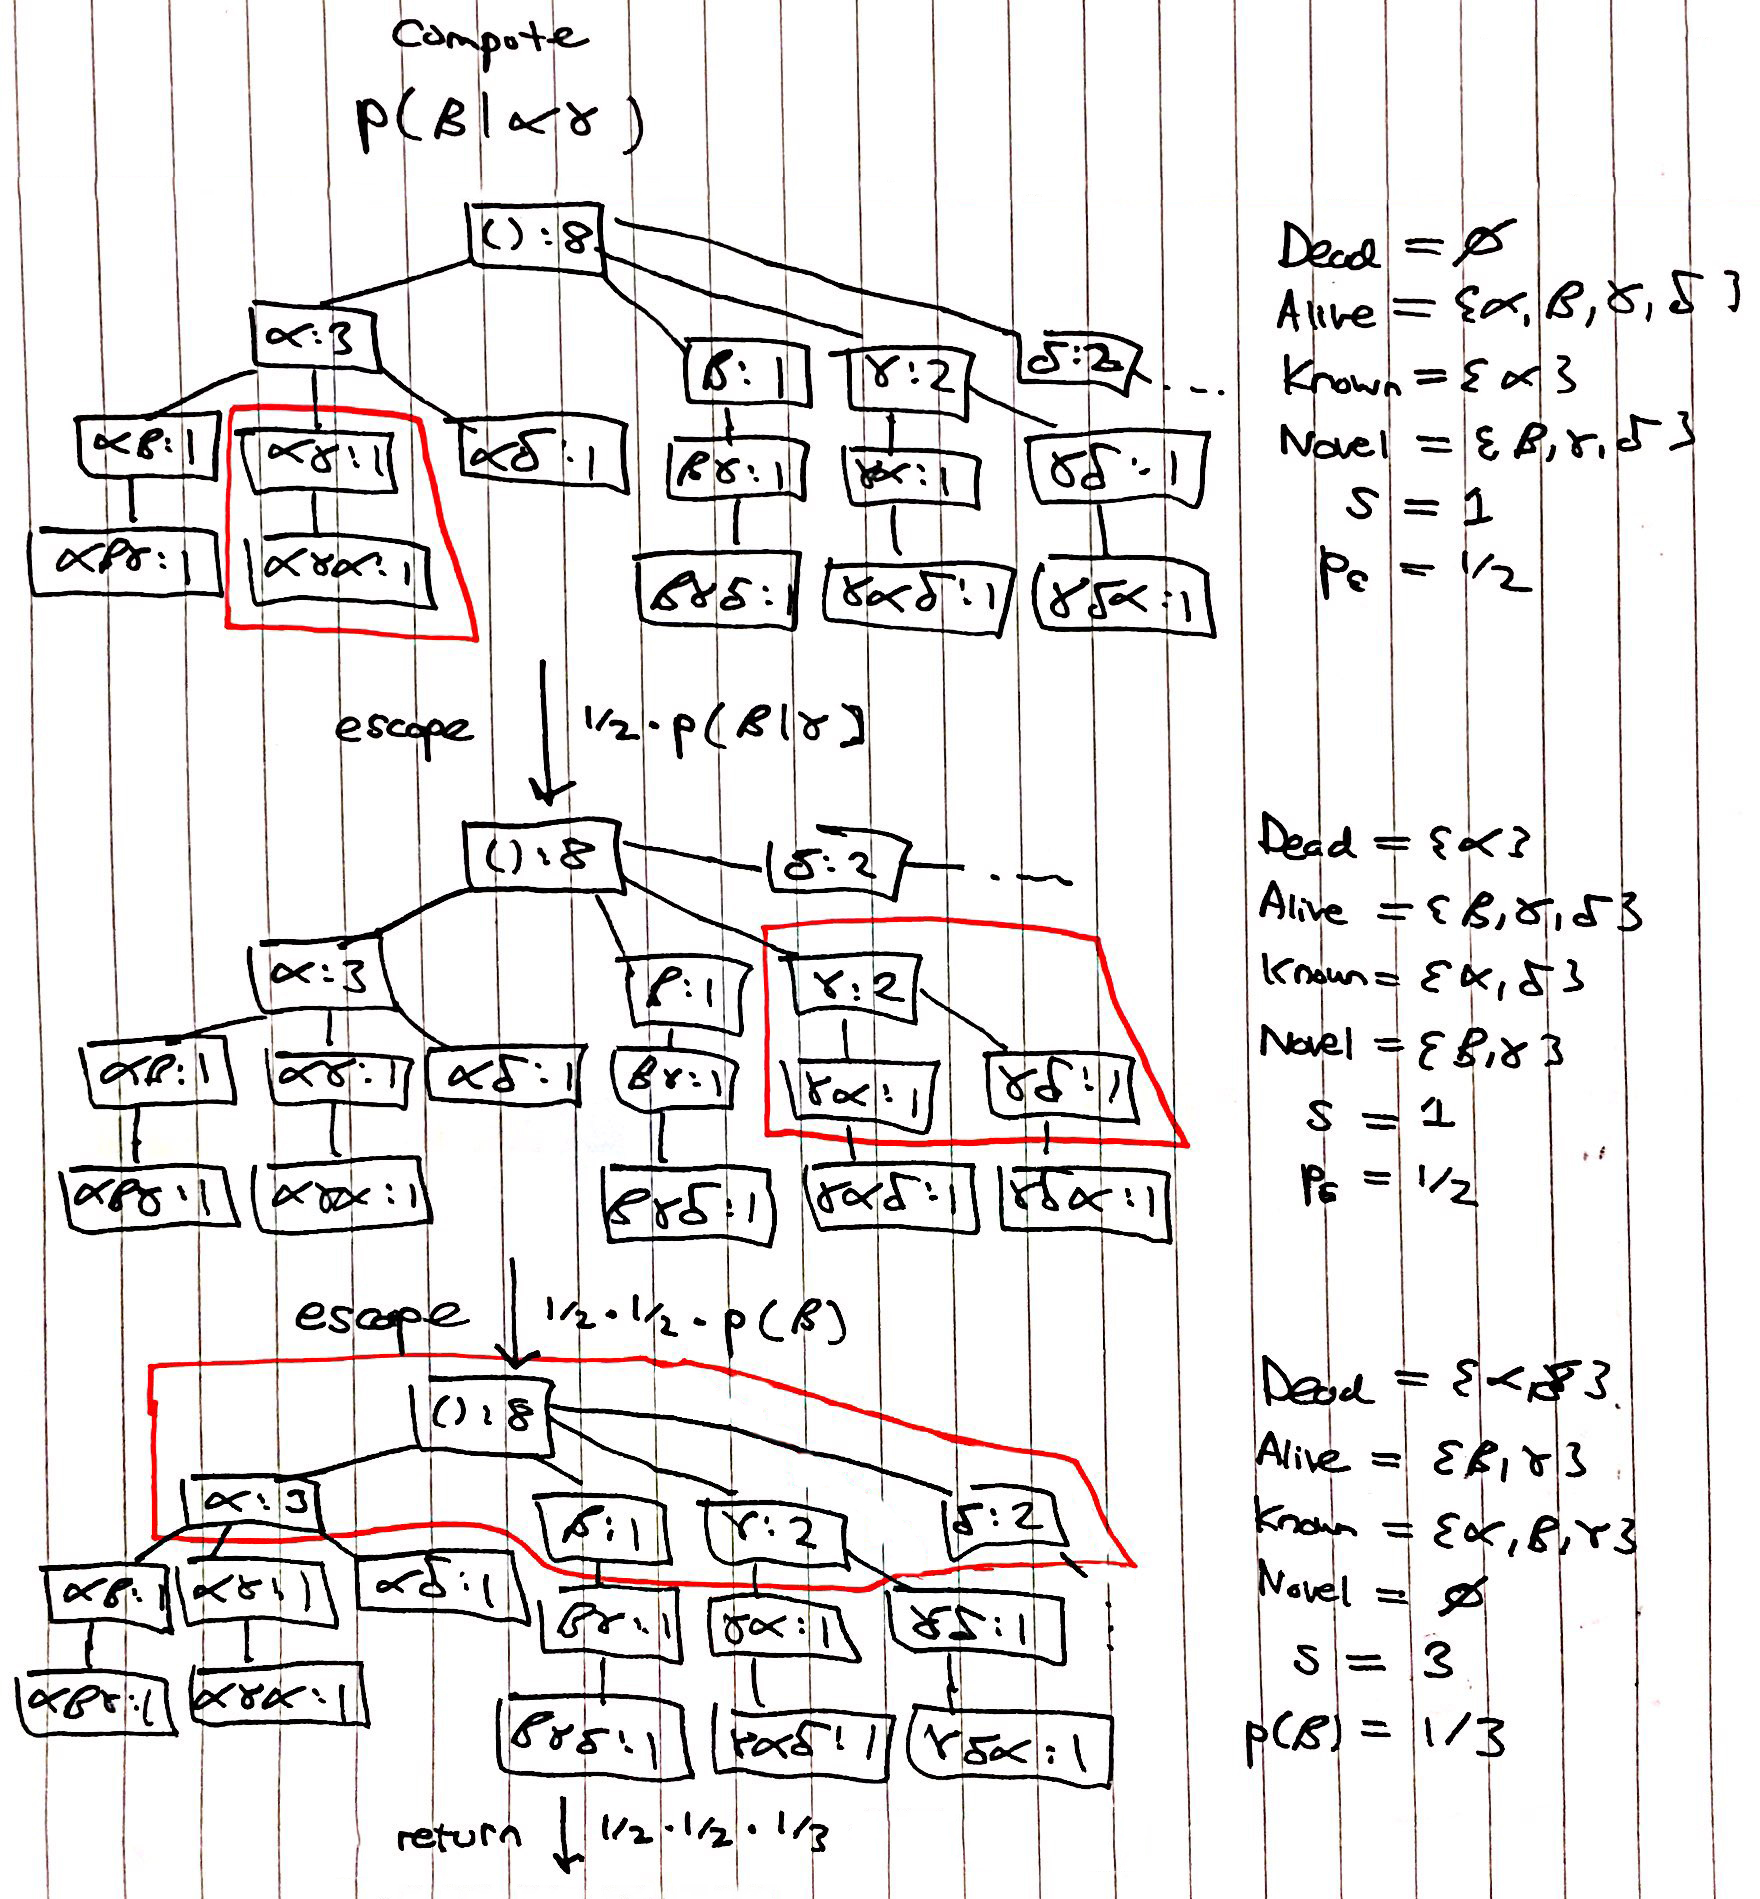
\includegraphics[width=400pt]{figs/ppm_stepwise_tmp.jpg}
\caption{Step-by-step execution of PPM with $\hbar = 3$ computing $p(\beta|\alpha\gamma)$}
\label{fig:ppm-stepwise}
\end{figure}

\subsection{Event Representation}\label{sec:cpp-event-rep}

In order to abstract the low-level \texttt{ContextModel} implementation and
generally to represent viewpoint types as first-class citizens in \texttt{C++},
a simple scheme was devised to represent viewpoint types as classes.

\begin{listing}[H]
  \begin{minted}[frame=single, linenos=true, fontsize=\footnotesize, mathescape]{cpp}
class T {
  const static cardinality; // set to $|[\tau]|$
  unsigned int encode();    // specifies the enumeration

  T(unsigned int c);        // construct using code $0 \leq c < |[\tau]|$
  T(const Other &o);        // construct using data 
};
  \end{minted}
  \caption{Prototypical viewpoint type representation}
  \label{lst:event-rep}
\end{listing}

To interface with the context model implementation, it suffices for each
viewpoint type $\tau$ to specify a well-known enumeration of $[\tau]$. The class
outlined in Listing~\ref{lst:event-rep} is a minimal example of how a class can
conform to this type representation convention.

Note that this is nothing more than a convention. Conformance to this convention
is not enforced \emph{explicitly} by any particular language feature. However,
if a class that does not conform to this convention is passed to a template
expecting a viewpoint type, this can still be caught at compile time due to
template substitution failure, e.g.\ when a template class attempts to access
\cppi{T::cardinality}.

Many templates in the implementation accept viewpoint types represented in this
way. I also chose to implement an iterator \texttt{EventEnumerator<T>} to
conveniently iterate over the members of a type in the style of the iterators in
the \texttt{C++11} standard template library, enabling clean loops such as~
\cppi{for (auto event : EventEnumerator<T>())}.

\subsection{Abstracting Context Models}

Now that we have established a scheme for representing viewpoint types, we can
abstract context models by providing an interface in terms of viewpoint types.
This is the job of a class which we call \texttt{SequenceModel}.  Specifically,
\texttt{SequenceModel<T>} is a wrapper class around an instance of
\texttt{ContextModel<T::cardinality>} for \texttt{T} a viewpoint type
represented as per Section~\ref{sec:cpp-event-rep}. 

Additionally, given some context, a \texttt{SequenceModel<T>} object can
generate probability distributions over subsequent events by iterating the
PPM implementation of the underlying context model for each member of
\texttt{T}. The object returned from this operation is an instance of
\texttt{EventDistribution<T>}, the functionality of which is discussed
in the following two sections.

It is desirable to provide an interface to context models in terms of viewpoint
types, since all other high-level classes in the implementation are
parameterised on types. Any viewpoint class modelling an underlying type
\texttt{T} can therefore simply instantiate a \texttt{SequenceModel<T>} object.

\subsection{Distribution Combination}

As mentioned in Section~\ref{sec:vp-comb}, there are various techniques for
combining probability distributions in a multiple viewpoint system. In line with
the agile development methodology, I initially implemented an entropy-weighted
arithmetic combination scheme in order to get a working result at an early
stage. Later, on the basis of its superior performance
(Section~\ref{sec:vp-comb}), I decided to implement a geometric scheme for
viewpoint combination.  

In order to cleanly express distribution combination with a standard interface,
yet allow the choice of a different underlying implementation, I utilised the
\emph{Strategy} pattern of object-oriented design
(Figure~\ref{fig:dist-strategy-uml}).

\begin{figure}[H]
\centering
  \trimbox{0cm 0.0cm 0cm 0cm}{ 
  \begin{tikzpicture}
  
  \umlclass[type=interface, template={$T$}, alias=strat]{DistCombStrategy}{}{
  + combine(list$\langle$EventDistribution$\langle T \rangle\rangle$) :
  EventDistribution$\langle T \rangle$
  }
  \umlsimpleclass[y = -4, x=-5, template={$T$}, alias=arith]{ArithmeticComb}
  \umlsimpleclass[y = -4, x=0, template={$T$}, alias=geo]{GeometricComb}
  \umlsimpleclass[y = -4, x=5, template={$T$}, alias=loggeo]{LogGeoComb}
  
  \umlimpl{arith}{strat}
  \umlimpl{geo}{strat}
  \umlimpl{loggeo}{strat}
\end{tikzpicture}
}
\caption{UML Class Diagram illustrating use of Strategy design pattern}
\label{fig:dist-strategy-uml}
\end{figure}

\texttt{ArithmeticComb} is a direct implementation of the weighted arithmetic
formula given in Section~\ref{sec:vp-comb}. \texttt{GeometricComb} is a direct
implementation of Pearce's weighted geometric formula
(\ref{eq:pearce-geometric}) , but this was found to suffer from numerical
instability. This was detected in the form of extremely high, or in some cases,
infinite cross-entropy on the test set. 

\begin{equation}
p(j) = \frac{1}{Z} \left( \prod_{i = 1}^N p_i(j)^{w_i} \right)^{ \frac{1}{
\sum_{i = 1}^N w_i }} \label{eq:pearce-geometric}
\end{equation}

The multiplication of many small exponentiated probabilities as per
(\ref{eq:pearce-geometric}) can yield an intermediate value too small to
represent in a \texttt{double}. Suppose, however, that we were able to represent
such an intermediate result. Then, raising it to a sufficiently small power
could certainly give an output large enough to represent in a \texttt{double}.
This suggests that the numerical issues might in fact be avoidable.

To mitigate this instability, I derived an alternative formulation of this
method as follows. Letting $\widetilde{p}(j)$ denote the unnormalised
probability for the $j$\textsuperscript{th} event, we find:
\begin{align*}
  \widetilde{p}(j) &= \left( \prod_{i=1}^N p_i(j)^{w_i}
  \right)^{\frac{1}{\sum_{i=1}^N w_i}} \\[3mm]
  \implies \ln{\widetilde{p}(j)} &= \frac{1}{\sum_{i = 1}^N w_i} \left( \sum_{i
  = 1}^N w_i \ln{p_i(j)} \right) \\[3mm]
  \implies p(j) &= \frac{1}{Z} \exp \left( \frac{\sum_{i = 1}^N w_i \ln{ p_i(j)
  }}{ \sum_{i = 1}^N w_i } \right).
\end{align*}

\texttt{LogGeoComb} implements a geometric combination using this new
expression: the probabilities are first added in log space and then
exponentiated and normalised. This was found to remedy the issues with numerical
stability entirely.

Figure~\ref{fig:num-instab} demonstrates this instability by plotting the
following functions in a critical region:
\begin{align*}
  f_1(x) &= 10^8 \left( \left( 10^{-8} \right)^x \right)^{1/x} \\
  f_2(x) &= 10^8 \exp( x \ln{10^{-8}} / x)
\end{align*}
where $f_1$ is representative of directly performing a geometric combination of
$x$ small probabilities and $f_2$ the sum-of-logs formulation. Clearly, both
$f_1$ and $f_2$ should be unity for all $x \in \mathbb{R}^+$. However, as
Figure~\ref{fig:num-instab} demonstrates, as $(10^{-8})^x$ becomes too small to
represent, $f_1(x)$ breaks down.

\begin{figure}[H]
\centering
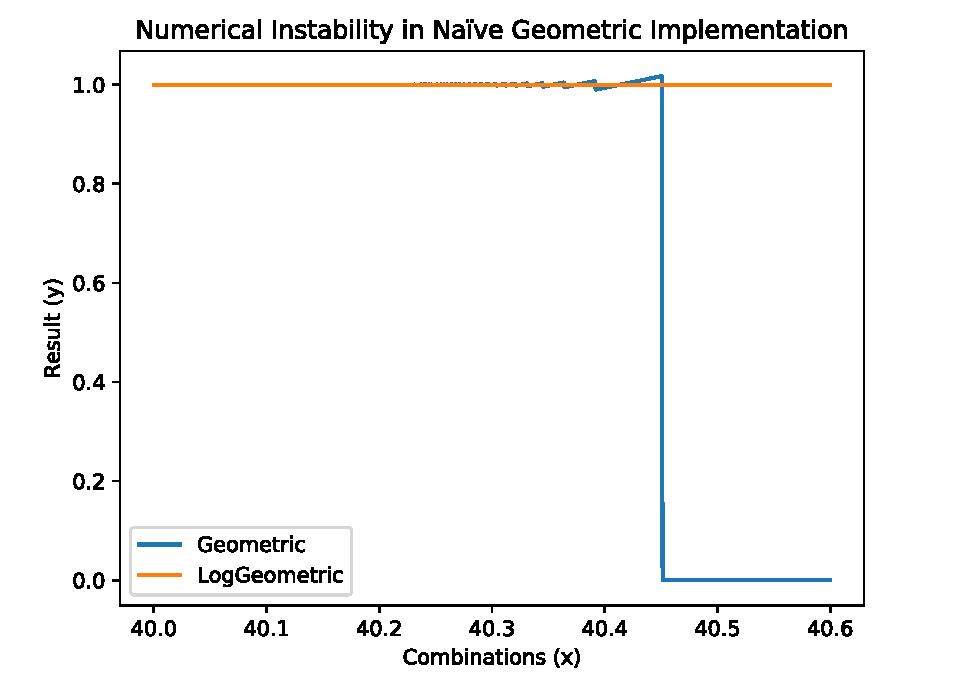
\includegraphics[width=400pt]{figs/instability.pdf}
\caption{Example of Numerical Instability in Naïve Geometric Combination}
\label{fig:num-instab}
\end{figure}

\subsection{Sampling from Distributions}

In order to sample from probability distributions, a high-quality source of
randomness is needed. After an initial investigation of the pseudo-random number
generators (PRNGs) available in the \texttt{C++11} standard library, I found
several other PRNGs that were shown to be superior in both performance and
statistical quality. Of these, I chose to implement \texttt{xoroshiro128+}, the
successor to the well-known \texttt{xorshift128+} PRNG \cite{vigna2017further}.
As of this writing, \texttt{xoroshiro128+} has been found to pass more
statistical tests than any other PRNG, including those available in the
\texttt{C++11} standard library\footnote{http://xoroshiro.di.unimi.it}. 

The implementation used the publicly-available reference C
code\footnote{http://xoroshiro.di.unimi.it/xoroshiro128plus.c} wrapped in a
\texttt{C++11} \texttt{UniformRandomBitGenerator}, enabling its use as a random
number engine compatible with the \texttt{C++11} \texttt{<random>} library. The
implementation was made available for other \texttt{C++} developers in the form
of an open-source project on GitHub.

Sampling is performed using the \texttt{xoroshiro128+} implementation by
default, but an alternative random source can easily be configured. The PRNG is
seeded using the system's source of randomness, falling back to the
high-resolution time since boot when this is not available.

\subsection{Early Viewpoints}

The event space for the chorales, determined by our choice of encoding in
Section~\ref{sec:corpus-prep-analysis}, is:
$$ \zeta = [\mathrm{pitch}] \times [\mathrm{onset}] \times [\mathrm{duration}]
\times [\mathrm{keysig}] \times [\mathrm{timesig}]. $$

Recall that the type \emph{onset} specifies the quantised starting time of each
event within a sequence. A problem with using this event space directly when
modelling the chorales with multiple viewpoints is that $[\mathrm{onset}]$ is
not a finite set. In practice, one could ensure its finiteness by setting a
maximum possible length of piece. However, this solution is unsatisfactory, not
least because it bounds the length of possible compositions. Moreover, modelling
this type directly or in combination with other types is not likely to capture
any useful regularity, since it is a global property of each composition.

Instead, define the type \emph{rest} as follows:
$$ \Psi_{\mathrm{rest}}(e_1^k) \triangleq \begin{cases} 
  \Psi_{\mathrm{onset}}(e_1^k) -
  \Psi_{\mathrm{onset}}(e_1^{k-1}) - \Psi_{\mathrm{duration}}(e_1^{k-1}) & k > 1 \\
  \Psi_{\mathrm{onset}}(e_1^1) & \text{otherwise}
\end{cases} $$
and use:
$$ \zeta = [\mathrm{pitch}] \times [\mathrm{duration}] \times [\mathrm{rest}]
\times [\mathrm{keysig}] \times [\mathrm{timesig}] $$
which gives us an entirely local representation, with $[\mathrm{rest}]$ being a
small finite set. The conversion can be performed when the corpus is loaded into
the MVS. 

As suggested by our chosen corpus representation, we make the assumption that
types \emph{keysig} and \emph{timesig} remain constant throughout a single
sequence. Therefore, our task is to predict \emph{pitch}, \emph{duration}, and
\emph{rest} at each timestep. This gives rise to the first viewpoints that were
implemented: the \emph{basic viewpoints}. These viewpoints simply model
these basic types individually.

\texttt{BasicViewpoint<T>} is then just a simple wrapper around
\texttt{SequenceModel<T>} that conforms to \texttt{Predictor<ChoraleEvent, T>}.
Such viewpoints can be used to set a baseline for the performance of a multiple
viewpoint system: a MVS $\set{\mathrm{pitch}, \mathrm{duration}, \mathrm{rest}}$
simply implements a naïve independent $n$-gram approach.

\subsubsection{Derived Types}

We make use of two abstract interpretations of the pitch surface to improve
predictive performance. The difference in pitch between two consecutive notes,
known as the \emph{sequential interval}, which we abbreviate to \emph{seqint},
captures regularity that is invariant to the absolute pitch of notes. Define:
$$ \Psi_{\mathrm{seqint}}(e_1^k) \triangleq \begin{cases}
  \Psi_{\mathrm{pitch}}(e_1^k) - \Psi_{\mathrm{pitch}}(e_1^{k-1}) & k > 1 \\
  \bot & \text{otherwise} 
\end{cases}
$$
to specify the viewpoint \emph{seqint}. The process of lifting a sequence in
$[\mathrm{seqint}]^*$ from a sequence $e_1^k \in \zeta^*$ follows immediately
from this definition. However, the process of reifying a distribution over
\emph{seqint} to give a distribution over \emph{pitch} is less clear.
Algorithm~\ref{alg:reify-seqint} details this process. Note that we need a
context of at least one event so that the absolute pitch of the previous event
is known.

\begin{algorithm}[H]
  \caption{Reification algorithm for \emph{seqint}}
  \label{alg:reify-seqint}
  \begin{algorithmic}[1]
    \Function{reify}{$e_1^k \in \zeta^*$, $p_{\mathrm{seqint}} :
    \mathrm{dist}\langle\mathrm{seqint}\rangle$}
      \State \textbf{assert} $e_1^k \neq ()$
      \Comment might not be able to activate
      \State $p_0 \gets \Psi_{\mathrm{pitch}}(e_1^k)$
      \State $p_{\mathrm{pitch}} \gets \textbf{new}\
      \mathrm{dist}\langle\mathrm{pitch}\rangle$
      \For{$\delta p \in [\mathrm{seqint}]$}
        \State $p' \gets p_0 + \delta p$
        \Comment compute corresponding pitch
        \If{$p' \in [\mathrm{pitch}]$}
          \Comment ensure $p'$ valid pitch
          \State $p_{\mathrm{pitch}}(p') \gets p_{\mathrm{seqint}}(\delta p)$
        \EndIf
      \EndFor
      \State renormalise $p_{\mathrm{pitch}}$ if necessary
      \State \Return $p_{\mathrm{pitch}}$
    \EndFunction
  \end{algorithmic}
\end{algorithm}

It is necessary to check the normalisation of the new distribution, since we may
lose some probability mass from $p_{\mathrm{seqint}}$ in the case that it
predicts an invalid (out-of-range) pitch.

While the interval between two consecutive notes is a salient feature of melody,
another important feature in \emph{tonal} music is where a pitch lies with
respect to the \emph{tonal centre} of a melody. The tonal centre is a property
of the melody's key, and is really a \emph{pitch class} rather than a specific
pitch. To take this into account, we specify a minimum pitch in this pitch class
and work modulo $12$. This reference pitch is known in the MVS literature as the
\emph{referent} of a key.

\begin{table}[H]
  \centering
  \begin{tabular}{ r | l | l | l | l | l | l | l | l | l }
    $\Psi_{\mathrm{keysig}}(e_1^k)$ & -4 & -3 & -2 & -1 & 0 & 1 & 2 & 3 & 4 \\
    \hline
    $\Psi_{\mathrm{referent}}(e_1^k)$ & 8 & 3 & 10 & 5 & 0 & 7 & 2 & 9 & 4 
  \end{tabular}
  \caption{Table showing the derivation of \emph{referent} from basic type \emph{keysig}}
  \label{tab:keysig-to-ref}
\end{table}

Using the definition of the \emph{referent} type given by
Table~\ref{tab:keysig-to-ref}, we define the \emph{intref} type to be the
interval with the referent modulo 12:

$$ \Psi_{\mathrm{intref}}(e_1^k) \triangleq 
  (\Psi_{\mathrm{pitch}}(e_1^k) - \Psi_{\mathrm{referent}}(e_1^k))\
  \mathrm{mod}\ 12.
$$

Similarly, we can reify a distribution over \emph{intref} as follows:

\begin{algorithm}[H]
  \caption{Reification algorithm for \emph{intref}}
  \label{alg:reify-intref}
  \begin{algorithmic}[1]
    \Function{reify}{$e_1^k \in \zeta^*$, $p_{\mathrm{intref}} :
    \mathrm{dist}\langle\mathrm{seqint}\rangle$}
      \State \textbf{assert} $e_1^k \neq ()$
      \Comment might not be able to activate
      \State $r \gets \Psi_{\mathrm{ref}}(e_1^k)$
      \State $p_{\mathrm{pitch}} \gets \textbf{new}\
      \mathrm{dist}\langle\mathrm{pitch}\rangle$ 
      \Comment initialise to all zeros
      \For{$i \in [\mathrm{intref}]$}
        \For{$p_0 \in \set{48,60,72}$}
          \State $p' \gets p_0 + r + i$
          \If{$p' \in [\mathrm{pitch}]$}
            \State $p_{\mathrm{pitch}}(p') \gets p_{\mathrm{pitch}}(p') +
            p_{\mathrm{intref}}(i)$
          \EndIf
        \EndFor
      \EndFor
      \State renormalise $p_{\mathrm{pitch}}$ 
      \State \Return $p_{\mathrm{pitch}}$
    \EndFunction
  \end{algorithmic}
\end{algorithm}

Both of these viewpoints were initially implemented as specialised viewpoint
implementations; that is, there were separate classes \texttt{IntervalViewpoint}
and \texttt{IntrefViewpoint}, both implementing the
\texttt{Predictor<ChoraleEvent, ChoralePitch>} interface.

\subsection{Linked Viewpoints}\label{sec:impl-linked-vps}

As discussed previously, pitch and duration are almost never independent in
music. This motivates the use of linked viewpoints in a multiple viewpoint
system. I first implemented a generic \texttt{BasicLinkedViewpoint} class which
implements a linked viewpoint over arbitrary \emph{basic types}, in particular
enabling a viewpoint linking pitch and duration.

There are a few points to note about the implementation. Firstly, observe that
the formalism introduced in Section~\ref{sec:mvs-formalism} treats linked
viewpoints as inherently symmetric objects; that is, $\tau_1 \otimes \tau_2$
predicts both $\tau_1$ and $\tau_2$. However, in the implementation, I chose to
decouple these to allow the asymmetric use of linked viewpoints. Use the
notation $\tau_1 \rightarrow \tau_2$ to denote the linked viewpoint $\tau_1
\otimes \tau_2$ which predicts $\tau_2$.

The meta-type \texttt{EventPair<P,Q>} takes viewpoint types $P,Q$ and implements
a viewpoint type $T$ with $[T] = [P] \times [Q]$ which follows the convention of
Section~\ref{sec:cpp-event-rep} for representing viewpoint types in
\texttt{C++}. The underlying context model for a linked viewpoint over types $P$
and $Q$ is then an instance of \texttt{SequenceModel<EventPair<P,Q>>}.

To predict a distribution over either of the constituent types of a linked
viewpoint, one simply sums out the joint distribution over the other type: a
viewpoint $\tau_1 \rightarrow \tau_2$ predicts a distribution over $[\tau_1]
\times [\tau_2]$ and then marginalises to obtain a distribution over $[\tau_2]$.

While the ability to link basic types is useful, it would be better to be able
to link arbitrary combinations of basic and \emph{derived} types. However, the
derived types implemented thus far rely on a specialised viewpoint
implementation. To implement $\emph{seqint} \rightarrow \emph{duration}$, we
would need to implement a specific linked viewpoint for this combination of
types that performs the lifting and reification for \emph{seqint}.

\subsection{Generalised Viewpoints}

The insight that led to the development of a fully general viewpoint
implementation was to make the code for \emph{lifting} and \emph{reification} of
each type a property of the type itself. In addition, each derived type $\tau$
declares a \texttt{derived\_from} property, which gives the name of the type
from which $\tau$ is derived. 

Template meta-programming was then utilised to compute the surface type of any
type \texttt{T} at compile time. The surface type of a type \texttt{T} is
\texttt{T::derived\_from} if \texttt{T} is derived, and \texttt{T} otherwise.

These changes allowed the implementation of \texttt{GeneralViewpoint},
\texttt{GeneralLinkedVP}, and \texttt{TriplyLinkedVP}, the linked viewpoints
allowing linking of completely arbitrary types. These template classes perform
the appropriate lifting and reification depending on their inputs.

\begin{table}[H]
  \begin{tabular}{ r | l | p{4.55cm} | p{6.5cm} }
    Type $\tau$ & Predicts & Syntactic Domain $[\tau]$ & Interpretation \\ \hline
    pitch & pitch & $\set{60,\ldots,82}$ & MIDI Pitch of note \\
    duration & duration & $\{$1, 2, 3, 4, 6, 8, 12, 14, 16, 20, 24, 28, 32, 56,
    64$\}$ &
    Duration of note in semiquavers \\
    rest & rest & $\set{0,4,8,12,16,20}$ & Leading rest length in semiquavers \\
    keysig & - & $\set{-4,\ldots,4}$ & Number of sharps in key signature \\
    timesig & - & $\set{12,16}$ & Number of semiquavers in bar \\ \hline
    seqint & pitch & $\set{-12,-9,-8,\ldots,10,12}$ & Sequential melodic interval \\
    intref & pitch & $\set{0,\ldots,11}$ & Harmonic interval with referent \\
    posinbar & - & $\set{0,\ldots,15}$ & Position of event within bar \\
    fib & - & $\set{\texttt{false}, \texttt{true}}$ & \texttt{true} iff.\ event is first in bar \\
    fip & - & $\set{\texttt{false}, \texttt{true}}$ & \texttt{true} iff.\ event is first in piece \\
    ioi & - & $\{$1, 2, 3, 4, 6, 8, 12, 14, 16, 20, 24$\}$ & Consecutive onset
    difference
  \end{tabular}
  \caption{Complete List of Implemented Types}
  \label{tab:mvs-types}
\end{table}

Table~\ref{tab:mvs-types} shows all implemented types separated into basic and
derived types. All derived types other than \emph{seqint} and \emph{intref} are
non-predictive (they cannot be reified). These types are only useful when linked
with a predictive type.

\subsection{Hyperparameter Optimisation}\label{sec:mvs-hyperparams}

Following the architectural constraints of Section~\ref{sec:mvs-arch}, the
free hyperparameters in our model are:
\begin{enumerate}[label=(\arabic*), itemsep=0mm]
  \item The set of viewpoints used. \label{itm:set-vps}
  \item The value of $\hbar$ (the order) for both the long- and short-term
    model. \label{itm:hbar}
  \item The inter- and intra-layer bias parameters for distribution combination.
    \label{itm:bias-params}
\end{enumerate}

We can deal with \ref{itm:set-vps} by using an automatic viewpoint selection
algorithm. In particular, we implement a simple forward stepwise selection
algorithm to achieve this. For \ref{itm:hbar} and \ref{itm:bias-params} we use a
grid search, illustrated in Figure~\ref{fig:grid-search}. 

Empirically, the resulting surface for \ref{itm:bias-params} is convex at many
different settings of \ref{itm:hbar}. This supports the argument than we can
first optimise \ref{itm:hbar} and then optimise \ref{itm:bias-params}. However,
an important subtlety is that the setting of \ref{itm:hbar} and
\ref{itm:bias-params} can both potentially affect the set of viewpoints that
result from the selection algorithm.

A heuristic approach to choosing the hyperparameters, would therefore be to run
the selection algorithm for \ref{itm:set-vps}, optimise \ref{itm:hbar}, then
\ref{itm:bias-params}, and repeat until convergence. While this technique cannot
possibly hope to converge on a global optimum, it seems to work well in
practice.

\begin{figure}[H]
\centering
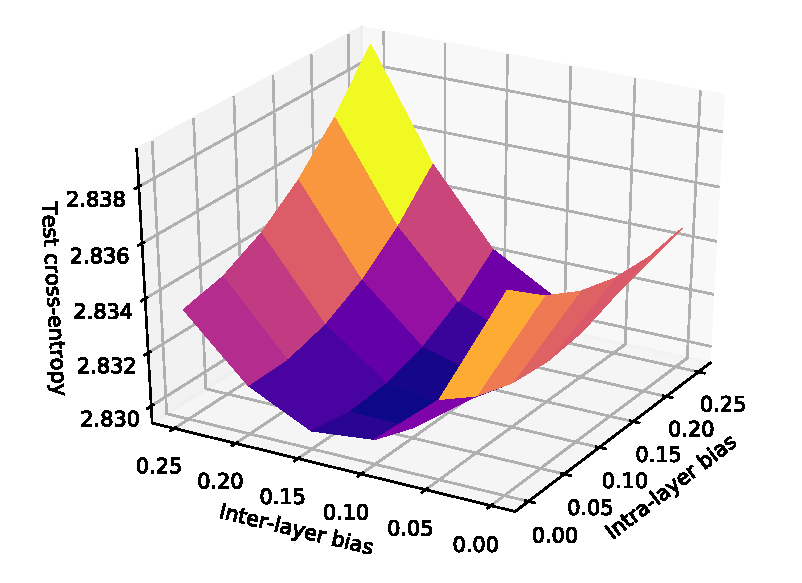
\includegraphics[width=350pt]{figs/bias_plot.pdf}
\caption{Grid search over bias parameters}
\label{fig:grid-search}
\end{figure}

\subsubsection{Automatic Viewpoint Selection}

A forward stepwise selection algorithm was implemented for choosing a suitable
set of viewpoints from some large pool of candidate viewpoints. This procedure
is detailed in Algorithm~\ref{alg:vp-select}. Along with a pool of viewpoints,
a test set for evaluating the candidate viewpoint systems is required. A fixed
parameter $\epsilon \in \mathbb{R}^+$ controls the minimum margin of improvement
necessary to accept a candidate viewpoint.

\begin{algorithm}[H]
  \caption{Viewpoint selection algorithm}
  \label{alg:vp-select}
  \begin{algorithmic}[1]
    \Function{optimise$\langle\tau\rangle$}{vp-pool, test-set, $\epsilon \in \mathbb{R}^+$}
      \State $S \gets$ \textbf{new}
      stack$\langle$predictor$\langle\tau\rangle\rangle$ 
      \Comment viewpoint stack
      \State $S$.push(basic-vp$\langle\tau\rangle$)
      \State $\mathcal{L}_{\mathrm{prev}} \gets$ evaluate($S$, test-set)
      \Comment baseline loss
      \Loop
        \State $\mathcal{L}_{\mathrm{round}} \gets \infty$
        \For{$V \in$ vp-pool}
          \If {$V \in S$} \textbf{continue}
          \EndIf
          \State $S$.push($V$)
          \State $\mathcal{L} \gets$ evaluate($S$, test-set) 
          \Comment evaluate candidate viewpoint $V$
          \If{$\mathcal{L} < \mathcal{L}_{\mathrm{round}}$}
            \State $\mathcal{L}_{\mathrm{round}} \gets \mathcal{L}$
            \State $V_{\mathrm{round}} \gets V$
          \EndIf
          \State $S$.pop()
        \EndFor
        \If{$\mathcal{L}_{\mathrm{prev}} - \mathcal{L}_{\mathrm{round}} >
        \epsilon$}
          \State $S$.push($V_{\mathrm{round}}$)
          \Comment accept $V_{\mathrm{round}}$, continue
        \Else
          \State \Return $S$
          \Comment no significant improvement, stop
        \EndIf
      \EndLoop
    \EndFunction
  \end{algorithmic}
\end{algorithm}

The best-performing MVS was found to have the following hyperparameters:
\begin{itemize}
  \item Viewpoints combined using geometric combination with bias set to $0.1$.
  \item A history parameter of $6$ for viewpoints in both long- and short-term model.
  \item The following viewpoint sets (using the notation of
    Section~\ref{sec:impl-linked-vps}):
\begin{verbatim}
pitch: { 
  pitch, (fib x duration)->intref, duration->seqint, (fib x ioi)->pitch,
 (fib x rest)->intref, (fib x duration)->pitch, ioi->seqint,
  duration->intref, posinbar->pitch, intref->seqint
}
duration: {
 duration, posinbar->duration, (fib x pitch)->duration,
 (fib x rest)->duration
}
rest: {
 rest, (fib x duration)->rest, (fib x intref)->rest
}
\end{verbatim}

\end{itemize}

\section{Recurrent Neural Network}

\subsection{Overview}

A multi-layer LSTM recurrent neural network (RNN) was implemented in Python
using TensorFlow \cite{abadi2016tensorflow}. The network uses \emph{dropout} for
regularisation as per Zaremba et al.\ \cite{zaremba2014recurrent}. A decoupled
``front-end'' to the RNN was implemented which allows the same internal model to
be used for character-level language modelling and music modelling. Random walk
sampling was implemented for generation. In addition, modifications to the
conventional sequence-prediction RNN architecture were made by feeding the
network additional \emph{global} musical information at each timestep, which was
found to improve performance significantly.

As a precursor to implementing a RNN for music modelling, I decided to implement
a recurrent network and apply it to the well-studied task of character-level
language modelling. This decision was made in the hope that the performance of
the network on a well-studied task would be a good indicator of the correctness
of the implementation, as well as to gain an appreciation of the effects of
tuning the hyperparameters on the performance of the model.

Since I chose to use TensorFlow to implement the RNN, this necessitated the use
of Python. Unfortunately, because Python uses a dynamic type system, many
programmer errors that could be caught at load time are instead caught at
runtime. This can lead to a significant amount of wasted time, especially when
the errors in a script occur following a lengthy computation. 

To improve on this situation, I utilised Python 3.6's \emph{type annotations}
along with the static type checker \texttt{mypy}\footnote{http://mypy-lang.org}
which was found to be highly effective at catching errors statically and improving
the overall efficiency of development in Python.

\subsection{Input Representation}

Before implementing the RNN model itself, I first implemented a module to ingest
and manage data from corpora. Specifically, this \texttt{DataLoader} module
takes a source corpus (in the form of a \texttt{txt} file for language modelling
or \texttt{JSON} file for music) and determines a \emph{vocabulary} $\Sigma$ for
the source. The source is then encoded using an enumeration of $\Sigma$ and
split into mini-batch matrices. 

\begin{figure}[H]
\centering
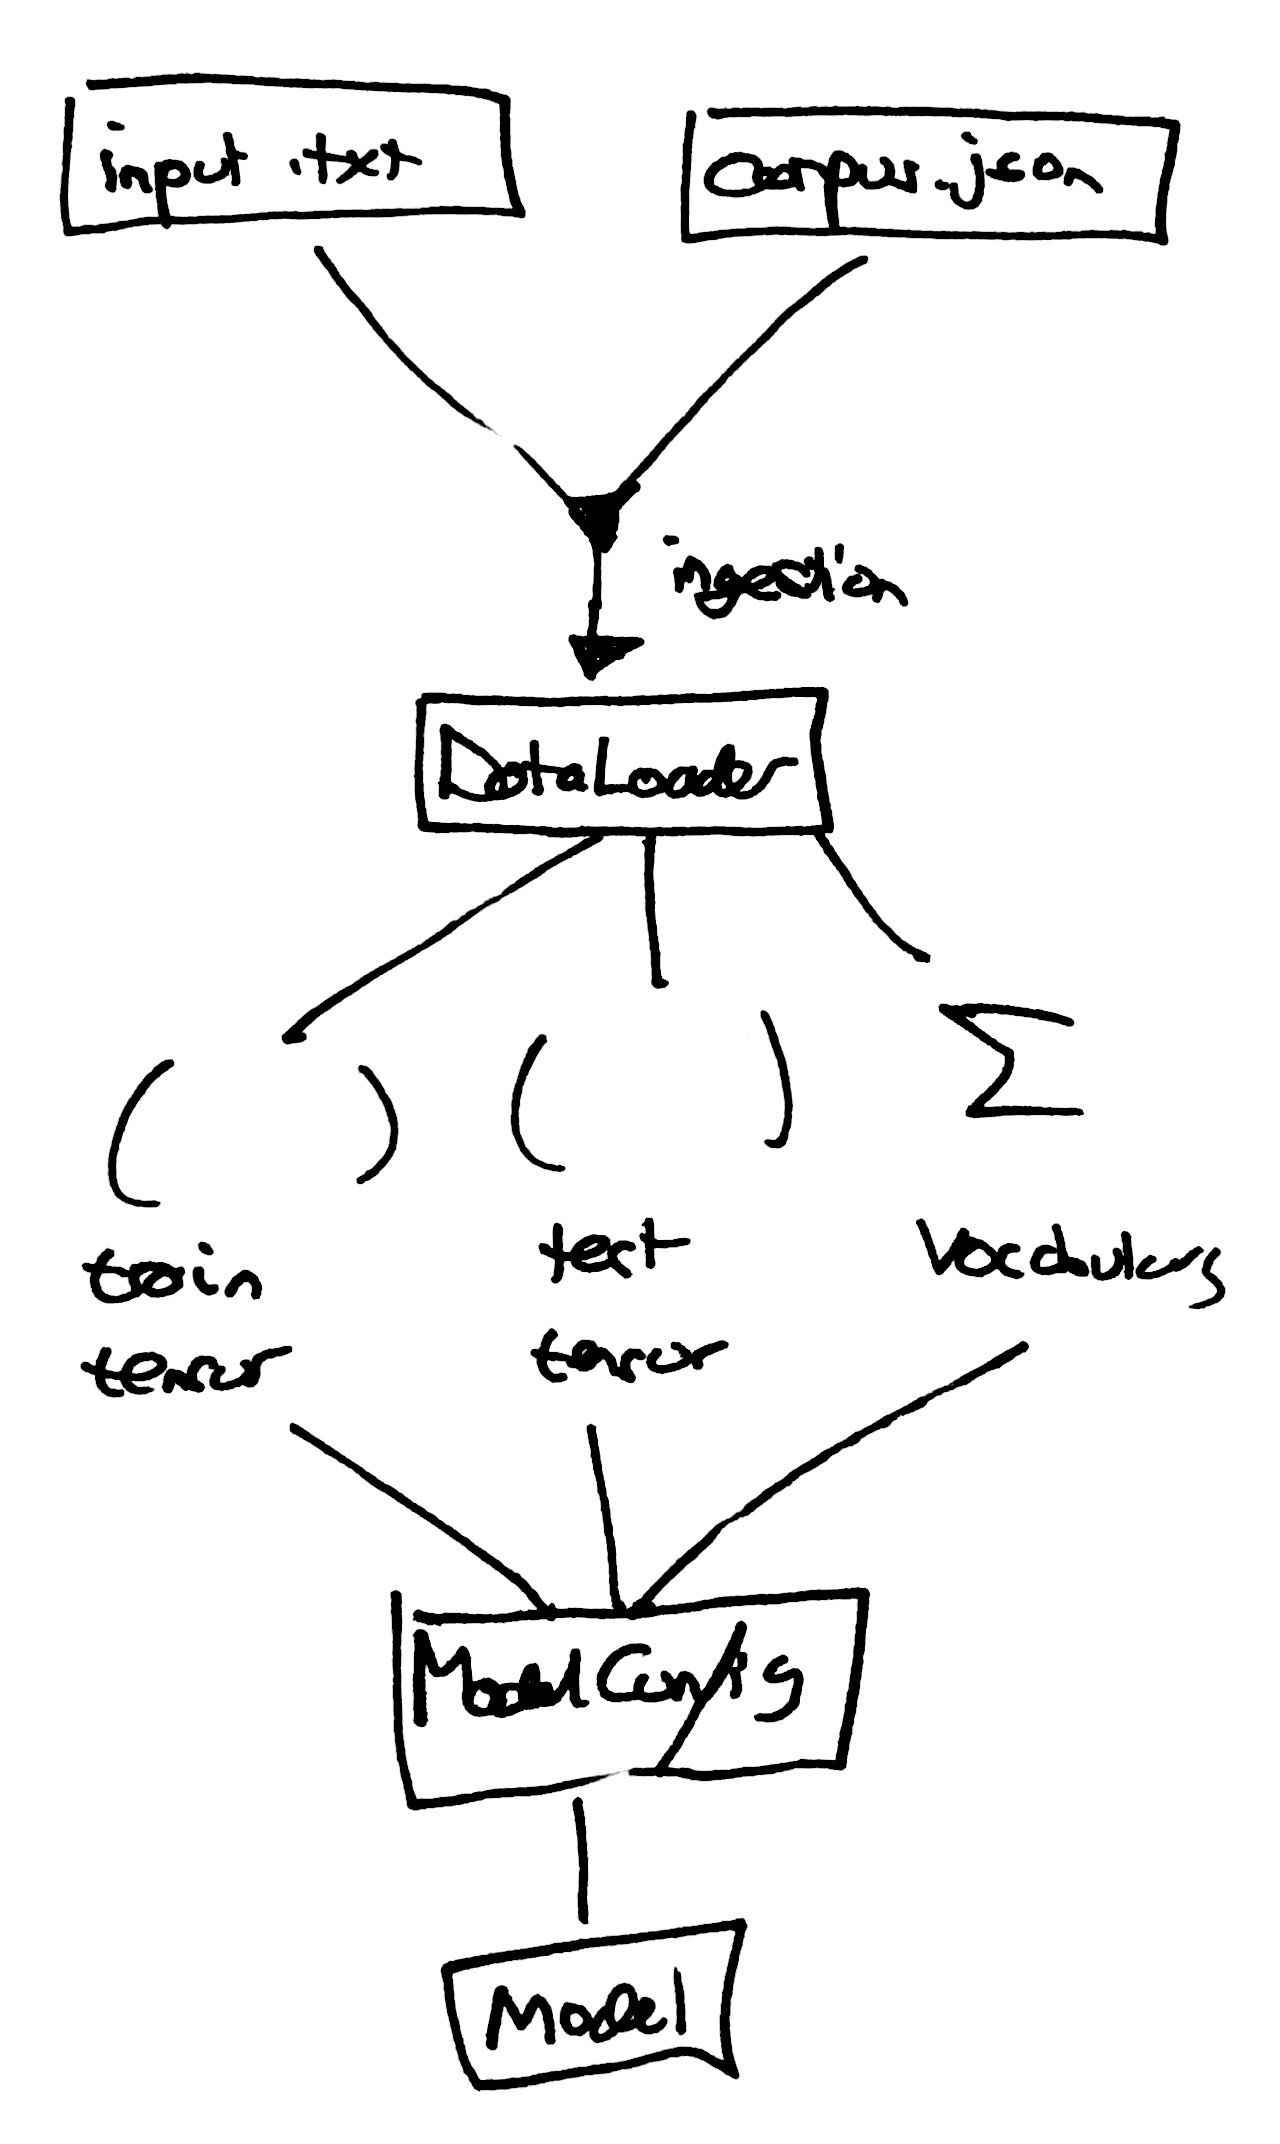
\includegraphics[width=200pt]{figs/rnn_frontend.jpg}
\caption{RNN front-end}
\label{fig:rnn-frontend}
\end{figure}

Importantly, the \texttt{DataLoader} module manages train and test data
separately: in the case of language modelling, $10\%$ of the text is kept aside
as test data. I chose to delegate the train/test split of musical data
to the corpus preparation stage since this needs particular care. The split is
therefore specified in the \texttt{JSON} file. 

Since Bach harmonised many chorale tunes multiple times (with slight variations
or in different keys), very similar melodies may appear in the corpus. Thus, the
train/test split of the corpus must ensure that the sets of chorale melodies in
the train/test sets are entirely disjoint.

\subsection{Core Model Implementation}

To discuss the core RNN implementation, we consider each of the hyperparameters
in turn and describe the corresponding functionality in the model.

\subsubsection{Model Structure}

Two parameters control the model complexity directly. The number of layers in
the deep RNN is controlled by a parameter \texttt{num\_layers}, and the size of
the LSTM state vectors is governed by \texttt{hidden\_size}.

The LSTM model definition uses the default TensorFlow implementation since this
is readily available. The \texttt{BasicLSTMCell} class is simply a convenient
wrapper around a handful of TensorFlow graph operations to define an LSTM cell
as introduced in Section~\ref{sec:lstm-prep}. 

\begin{listing}
  \begin{minted}[frame=single, linenos=true, fontsize=\footnotesize,
  mathescape]{python}
lstm_cell = tf.nn.rnn_cell.BasicLSTMCell(hidden_units, state_is_tuple=True)
cells = [lstm_cell] * config.num_layers
self.cell = tf.nn.rnn_cell.MultiRNNCell(cells, state_is_tuple=True)
  \end{minted}
  \caption{LSTM Definition in \texttt{Model} Class}
\end{listing}

The only difference with the LSTM as introduced previously is that the
TensorFlow LSTM implementation adds a bias of $1$ to the forget gate layer. This
prevents forgetting towards the beginning of training, which is useful in
practice.

The dimensionality of much of the input I/O is governed by the parameters
\texttt{batch\_size} and \texttt{vocab\_size} which are determined by the
\texttt{DataLoader} class. For simplicity, I chose to unfold the RNN to a fixed
size, specified by the parameter \texttt{seq\_length}.

\subsubsection{Training}

To mitigate the effects of the \emph{exploding gradient problem}, introduced in
Section~\ref{sec:rnn-train}, I globally clip the norm of gradients in the
network to some maximum value given by the hyperparameter
\texttt{max\_grad\_norm}. This is a technique utilised by e.g.\ Graves in 2013
\cite{graves2013generating}.

The network is trained by stochastic gradient descent. Specifically, the
training data are split into mini-batches during ingestion. At train time, the
gradient is computed using each mini-batch in turn to complete an \emph{epoch}
of training (an entire pass through the data). The total number of epochs
performed in a session is given by the \texttt{num\_epochs} parameter.

I chose to implement a learning rate schedule of exponential decay. This enables
large changes in the parameters to be learned towards the start of training and
more fine-tuned adjustments to be made towards the end of training. In
particular, I adapt the learning rate as:
$$ \alpha_e \gets \epsilon\alpha_{e-1} $$
where $\alpha_e$ is the learning rate at epoch $e$ and $0 < \epsilon < 1$ is a
decay parameter which we call \texttt{lr\_decay}. We fix $\alpha_0$ with a
hyperparameter \texttt{learning\_rate}.

\subsubsection{Regularisation}

\emph{Dropout} \cite{srivastava2014dropout} is a powerful technique for
preventing overfitting in deep feedforward networks which works by randomly
shutting off some fraction of the units in some or all of the layers at train
time. This prevents excessive co-adaption among units in the network.

A recent paper by Zaremba et al.\ \cite{zaremba2014recurrent} made a major
contribution by showing how to apply dropout successfully to recurrent networks.
Although attempts had been made to apply dropout to RNNs prior to this work,
they were largely unsuccessful. In particular, applying dropout to the
\emph{recurrent} connections in a RNN leads to poor performance.

The authors found that applying dropout only to the non-recurrent connections
successfully prevents overfitting in a recurrent network and lead to improved
performance on a number of tasks. In the context of the LSTM formulation of
Section~\ref{sec:lstm-prep}, we replace:
$$ \vect{x} = [\vect{h}_{t-1}^l, \vect{h}_t^{l-1}] $$
with
$$ \vect{x} = [\vect{h}_{t-1}^l, \mathrm{D}_p(\vect{h}_t^{l-1})] $$
for equations (\ref{eq:lstm-f}) through (\ref{eq:lstm-d}), where $\mathrm{D}_p$
is the \emph{dropout operator} which randomly sets each component in its result
vector to zero with probability $p$, but otherwise returns its input. 

\subsection{Language Modelling Experiments}

As mentioned earlier, initial experiments were performed on a task of language
modelling. This was done as an indicator of the correctness of the
implementation and to gain an appreciation of the effects of each of the
hyperparameters.

Initial experiments on a dataset of the first ``Harry Potter'' book found raw
predictive performance to increase with the hidden state size (\todo tabulate)
for a single-layer LSTM network.

\begin{verbatim}
epochs: 20, hidden: 32,  lrd: 0.7, loss: 167
epochs: 20, hidden: 64,  lrd: 0.7, loss: 148
epochs: 20, hidden: 128, lrd: 0.7, loss: 134
epochs: 20, hidden: 256, lrd: 0.7, loss: 121
epochs: 20, hidden: 512, lrd: 0.7, loss: 111
\end{verbatim}

Note that, at this point in time, the cross-entropy loss function was
unnormalised, meaning that the loss depended on the length of the unrolled RNN.
I later normalised the loss function to have units of
$\mathrm{bits}/\mathrm{event}$ which enabled direct comparisons between models.

The following is an excerpt of a generated sample from the best-performing of
these single-layer models which demonstrates having learned long-term
dependencies in the form of the high-level structure:

\begin{displayquote}
Come on, how faces repaired his goal ohth, which she felt himself staring up and
down before the squeaking bottom, twitching, on his trunk and a package of
Harry's face.

``Well... for a last few hours - Dumbledore --''

But Malfoy dived it.

``Professor -- Scabbers backed in to my family!''
\end{displayquote}
\vspace{4mm}

Initially, some difficulty was experienced in training deep RNNs. In particular,
using $20-30$ epochs of training with the \texttt{lr\_decay} set to $0.7$,
multi-layer RNNs were outperformed by single-layer RNNs.

\subsection{Applying the RNN to Music}

Unlike the MVS implementation which predicts each event componentwise, the RNN
uses an event representation where each possible event in the musical event
space is encoded opaquely as a natural number: we do not present the structure
of events to the network.

Since the inputs are first embedded into the RNN's state space using a learned
embedding, the RNN can learn an event representaiton automatically.

Initial experiments on the chorale corpus showed that a single-layer RNN
achieved reasonable performance. 

Following the initial difficulty in training deep LSTMs, it was found that a
much less agressive learning-rate decay (between $0.95$ and $0.99$) and training
for many more epochs enabled two-layer LSTM networks to fit to the data better
than their single-layer counterparts. In fact, a 256-wide two-layer LSTM network
fit to the training set with almost zero loss: clearly, there was some
overfitting at play.

The presence of overfitting was immediately apparent from inspection of the
generated samples of such models: the network would quote entire fragments of
melody from the corpus.

\subsection{Tonality}

By inspecting the samples produced by RNNs trained on the base chorale corpus,
an immediate problem found was that the output was \emph{tonally unstable}. That
is, compositions will start in a particular key and wander into an unrelated
key: an effect that is both jarring to the listener and uncharacteristic of the
target genre.

This stemmed from the fact that the corpus contains compositions in many
different keys. The typical approach taken here is to normalise all of the
compositions by trasposing them into a common key.

\subsection{Metrical Coherence}

\todo Explain ``clock'' inputs. Discuss symmetry with multiple viewpoints.

\subsection{Hyerparameters}

The best-performing recurrent neural network (RNN) used a semiquaver-level clock
and was trained on the corpus with tonal inflation of $\pm 5$. The model had two
LSTM layers with a state dimensionality of 256. Dropout was used for
regularisation between these two layers with the probability $0.5$.  After
training the network for 110 epochs with a learning-rate decay of $0.95$ and
initial learning rate of $1.0$, the network obtained its optimal loss on the
test set.

\section{Testing and Debugging}

\todo Get lots of points and stickers for demonstrating good software
engineering practice by testing thoroughly.

\chapter{Evaluation}\label{chap:eval}

The goal of the evaluation of this work is to compare the performance of the two
implemented techniques, the multiple viewpoint system (MVS) and recurrent neural
network (RNN), on the task of generating chorale-like melodies.

The first important issue to address in undertaking this is specifying what is
meant by \emph{performance} with respect to melody generation. As with any art
form, the success of a music generation system in the abstract sense is not
something that can be specified objectively. However, one \emph{can} objectively
investigate:
\begin{itemize}
  \item The responses of many human participants to subjective evaluation
    criteria in an effort to generalise and draw conclusions about the opinions
    of many more people with respect to such criteria.  
  \item In the case of probabilistic models, such as those implemented, one can
    use objective metrics such as a \emph{cross-entropy} loss function to
    compare the predictive performance of models on unseen data. 

    Under the assumption that the predictive performance of a generative model
    is related to the quality of sampled outputs from the model with respect to
    the chosen subjective evaluation criteria, one can use such metrics as an
    indicator of generative performance. While there are good reasons to make
    this assumption, we do not rely on this metric in isolation.
\end{itemize}

\vspace{4mm}

We start by introducing an objective metric for comparing the \emph{predictive}
performance of the two techniques. Then, we compare the two techniques using
this metric, thereby selecting the models to take forward for further
evaluation. 

Then, after introducing and justifying subjective evaluation criteria for
generated outputs, we present and discuss an evaluation survey in which
participants listened to model outputs and responded to questions based on the
chosen evaluation criteria. We supplement this mass evaluation survey with
specific comments from an expert musicologist. Finally, we conclude by
summarising the results of the evaluation.

\section{Predictive Performance}

\subsection{Loss Function}

Recall from Section~\ref{sec:gen-models} that both techniques implemented in
this work approximate the joint distribution $p(\vect{x})$ over sequences
$\vect{x} = x_1,\ldots,x_t$ as follows:
$$ p(\vect{x}) = p(x_t | x_{t-1}, \ldots, x_1) p(x_{t-1} | x_{t-2}, \ldots, x_1)
\cdots p(x_1). $$
This allows the process of \emph{predicting} a sequence of length $T$ (assigning
probability to the sequence) to be broken down into $T$ steps. Namely, for $t
= 1$ to $T$, compute $p(x_t | x_{t-1}, \ldots, x_1)$ where $x_1, \ldots,
x_{t-1}$ are the known previous events in the sequence. 

Consider the $i$\textsuperscript{th} step of the prediction process. Our model
forms a distribution over possible subsequent events $x'$ in our event space
$\zeta$:
$$ p(x' | x_{i-1}, \ldots, x_1). $$
Suppose that we know the ``true'' underlying distribution $q(x' |
x_{i-1}, \ldots, x_1)$. Then the \emph{cross-entropy} between $p$ and
$q$ is given by:
$$ H(p,q) = - \sum_{x' \in \zeta} q(x' | x_{i-1}, \ldots, x_1) \log_2{ p(x' |
x_{i-1}, \ldots, x_1)}. $$
Of course, the underlying distribtuion $q(x' | x_{i-1}, \ldots, x_1)$ is not
known in practice. However, we can form the \emph{degenerate distribution}
$\widetilde{p}(x' | x_{i-1}, \ldots, x_1)$ which deterministically predicts the
test sequence $\vect{x}$:
$$ \widetilde{p}(x' | x_{i-1}, \ldots, x_1) \triangleq \begin{cases}
  1 & x' = x_i \\
  0 & \text{otherwise}
\end{cases} $$
Then, the cross-entropy of our model predicting $\vect{x}$ at timestep $t$ is
given by: 
$$ H(p,\widetilde{p}) = - \log_2{ p(x_t | x_{t-1}, \ldots, x_1) } $$
giving rise to the cross-entropy sequence loss function
$\mathcal{L}(\vect{x})$
which is the mean cross-entropy for the sequence with respect to our model:
$$ \mathcal{L}(\vect{x}) = - \frac{1}{T} \sum_{t = 1}^T \log_2{ p(x_t | x_{t-1},
\ldots, x_1) }. $$

Given an unseen test set $(\vect{x}_1,\ldots,\vect{x}_N)$, we then calculate the
mean cross-entropy loss:
$$ \frac{1}{N}\sum_{i = 1}^N \mathcal{L}(\vect{x}_i) $$
as a measure of the predictive performance of our model. Since the cross-entropy
at each timestep increases monotonically with $1/p$, it is a direct measure of
the error in our predictions. The logarithm yields losses that lie in a
manageable numerical range.

\subsection{Results}

When measuring predictive performance, we are interested in the ability of our
models to \emph{generalise} to unseen data. For this reason, we must ensure that
examples seen in training do not appear in the test set. In the case of our
corpus of melodies extracted from the chorale harmonisations of J.S.\ Bach,
ensuring a hygienic partition of the data into training and test sets is
non-trivial. Since Bach harmonised melodies multiple times with slight variation
in ornamentaiton and tonality, the data had to be partitioned based on the
underlying melody. To acheive this, the mapping between chorales and
harmonisations\footnote{Taken from the \emph{Riemenschneider} edition of Bach's
chorale harmonisations.} was encoded by hand in the corpus preparation script.

To compare the two techniques, we choose the best-performing model based on the
test loss. For the MVS, this was obtained using the hyperparamter optimisation
process of Section~\ref{sec:mvs-hyperparams}, while the RNN hyperparameters were
chosen by hand. 

With 95\% confidence, the MVS obtained a cross-entropy of $2.826 \pm 0.071\
\mathrm{bits}/\mathrm{event}$ on the test set, while the RNN achieved $3.017 \pm
0.078\ \mathrm{bits}/\mathrm{event}$. Thus, with $95\%$ confidence, the MVS
outperforms the RNN in terms of predictive ability. While this indicates that
the MVS might generate more successful outputs, this remains to be demonstrated.

\subsubsection{Analysis}
\vspace{-4mm}
\begin{figure}[H]
\centering
\subfloat[RNN (mean loss: $3.602\ \mathrm{bits}$)] {
  \label{subfig:rnn-aus-meines}
  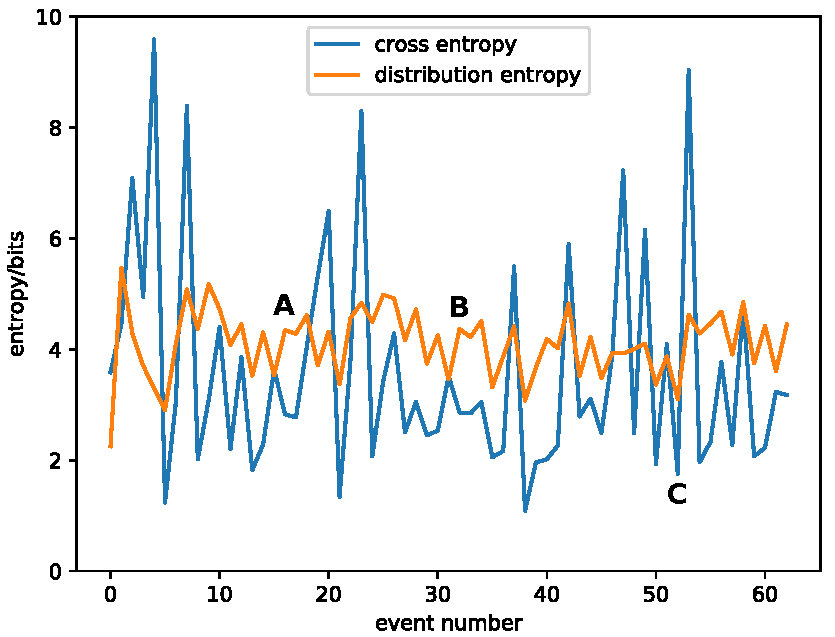
\includegraphics[width=220pt]{figs/rnn_aus_meines_profile.pdf}
}
\subfloat[MVS (mean loss: $3.332\ \mathrm{bits}$)] {
  \label{subfig:mvs-aus-meines}
  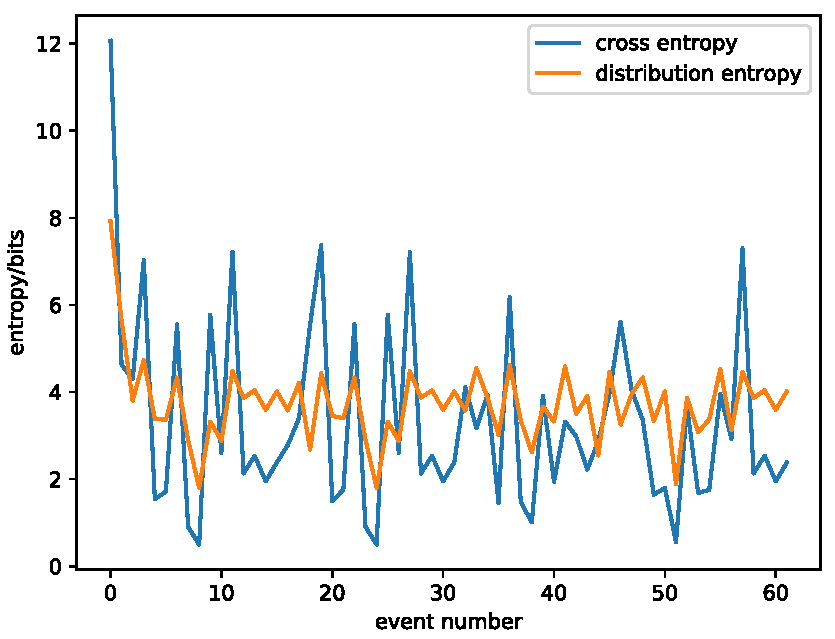
\includegraphics[width=220pt]{figs/mvs_aus_meines_profile.pdf}
}

\subfloat[Input chorale \emph{Aus Meines Herzens Grunde}] {
  \label{subfig:aus-meines-score}
  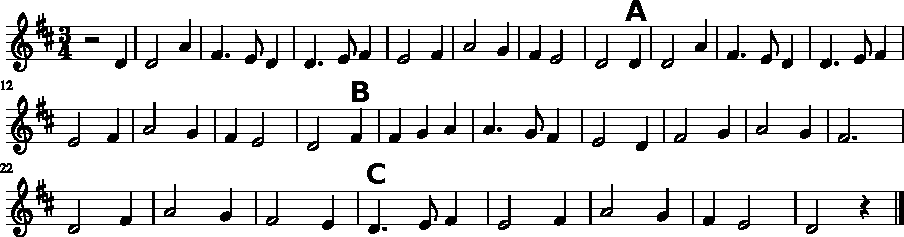
\includegraphics[width=0.8\linewidth]{figs/aus_meines_score.pdf}
}
\caption{Entropy profiles of models predicting representative unseen chorale}
\label{fig:aus-meines-profiles}
\end{figure}

While measuring the overall performance of each model in a single number is
useful, it is not particularly insightful. In this section, we take a more
fine-grained approach by looking at the \emph{entropy profile} of various
sequences with respect to each model. In each profile, we show the
cross-entropy: a measure of how poorly the model predicted each event, and the
distribution entropy: a measure of overall uncertainty in the prediction at each
point.

Figure~\ref{fig:aus-meines-profiles} shows a side-by-side comparison of the two
models on a melody from the test set. At position \textbf{A}, we have direct
re-use of the initial melodic material. At \textbf{B}, we have a related but
distinct middle section, and at position \textbf{C}, the opening material
returns. It can be seen that, in this case, the MVS predicts unseen material
more successfully than the RNN, while the RNN predicts re-used material slightly
better.

Figure~\ref{fig:danket-dem-profiles} gives an example where the MVS outperforms
the RNN. The note at position \textbf{A} is unexpected by both models, but
several orders of magnitude more so by the RNN. \textbf{B} indicates the start
of the second phrase, and \textbf{C} indicates the return of material from
\textbf{A}. In this case, unlike the RNN, the MVS predicts the re-used material
particularly well. This success might be attributable to the short-term model.

Figure~\ref{fig:als-der-profiles} shows one of the (few) examples where the RNN
outperforms the MVS. Some of the melodies in the corpus, such as this one, are
written with rests between phrases. The positions of the rests in the melody
are given by \textbf{A}, \textbf{B}, and \textbf{C}. It can be seen that the RNN
handles these better, in particular predicting the rest at position \textbf{C}
accurately.

\begin{figure}[H]
\centering
\subfloat[RNN (mean loss: $3.044\ \mathrm{bits}$)] {
  \label{subfig:rnn-danket-dem}
  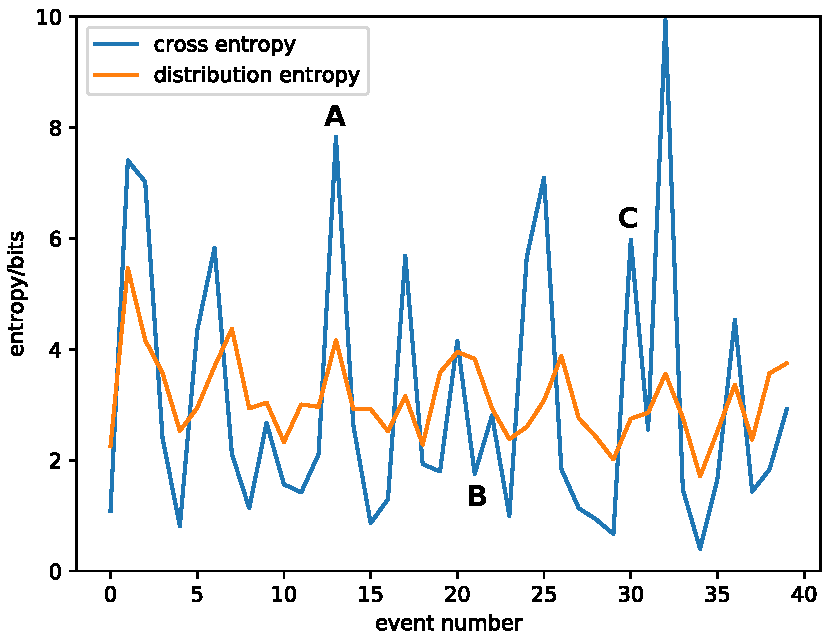
\includegraphics[width=220pt]{figs/rnn_danket_dem_profile.pdf}
}
\subfloat[MVS (mean loss: $1.849\ \mathrm{bits}$)] {
  \label{subfig:mvs-danket-dem}
  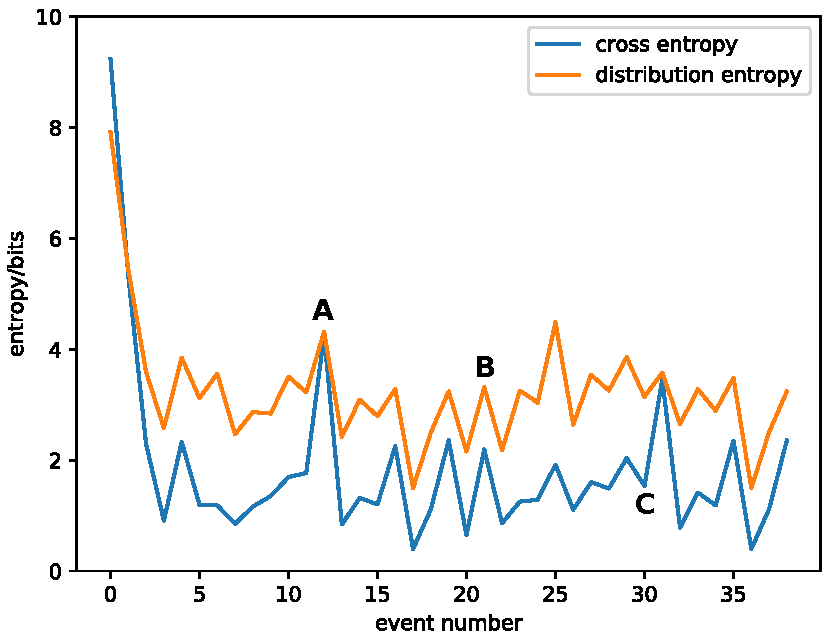
\includegraphics[width=220pt]{figs/mvs_danket_dem_profile.pdf}
}

\subfloat[Input chorale \emph{Danket dem Herrn heut und allzeit}] {
  \label{subfig:danket-dem-score}
  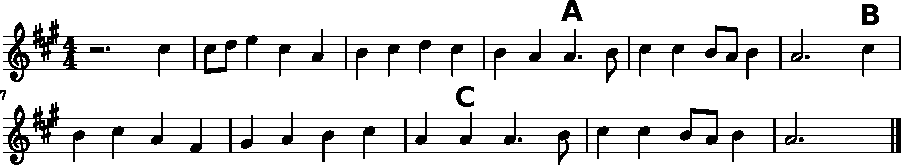
\includegraphics[width=0.85\linewidth]{figs/danket_dem_score.pdf}
}
\caption{Entropy profiles of chorale on which MVS significantly outperforms RNN}
\label{fig:danket-dem-profiles}
\end{figure}

\begin{figure}[H]
\centering
\subfloat[RNN (mean loss: $2.686\ \mathrm{bits}$)] {
  \label{subfig:rnn-als-der}
  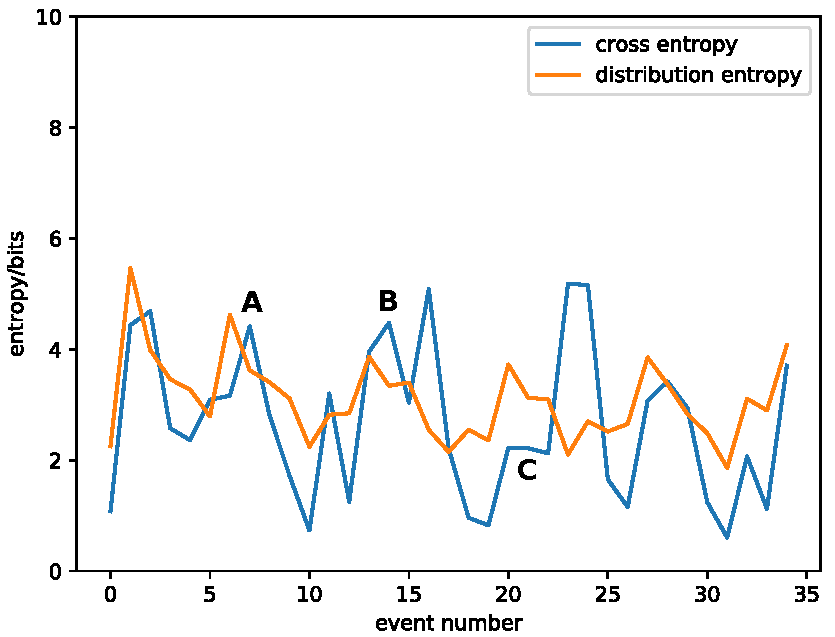
\includegraphics[width=220pt]{figs/rnn_als_der_profile.pdf}
}
\subfloat[MVS (mean loss: $3.031\ \mathrm{bits}$)] {
  \label{subfig:mvs-als-der}
  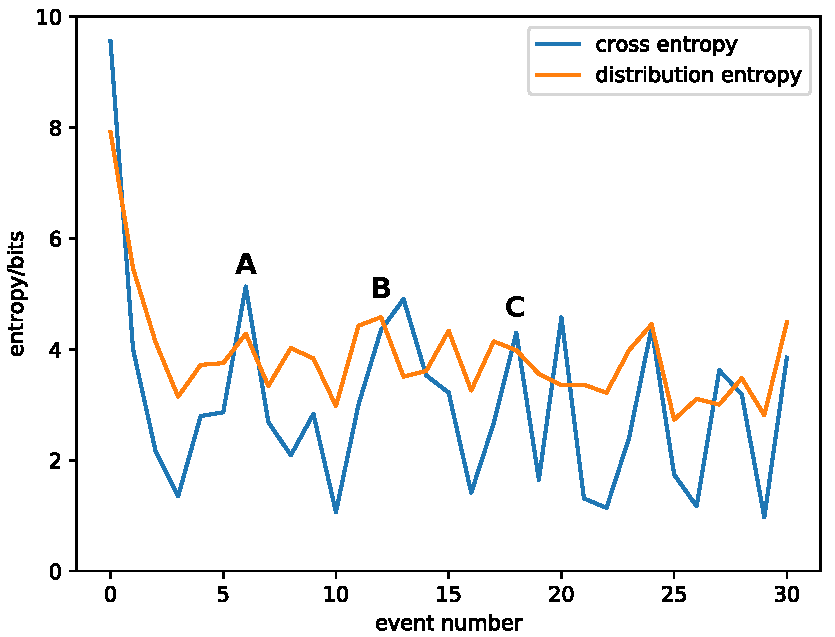
\includegraphics[width=220pt]{figs/mvs_als_der_profile.pdf}
}

\subfloat[Input chorale \emph{Als der gütige Gott vollenden wollt sein Wort}] {
  \label{subfig:als-der-score}
  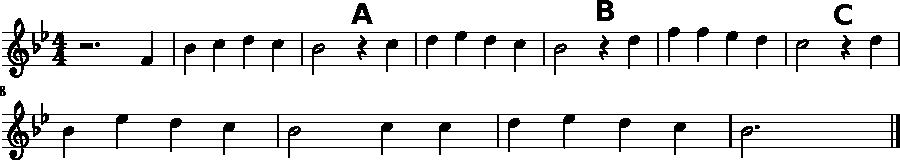
\includegraphics[width=0.85\linewidth]{figs/als_der_full.pdf}
}
\caption{Entropy profiles of chorale on which RNN outperforms MVS}
\label{fig:als-der-profiles}
\end{figure}

We expect our models to reject sequences that are clearly not in the chorale
genre. Models that do not do this may generate undesirable sequences when
sampled. Thus, it is useful to test how our models behave on pathalogical
inputs. Figure~\ref{fig:path-profiles} illustrates the behaviour of each model
when asked to predict a sequence of thirty identical notes. 

\begin{figure}[H]
\centering
\subfloat[RNN (mean loss: $2.566\ \mathrm{bits}$)] {
  \label{subfig:rnn-path}
  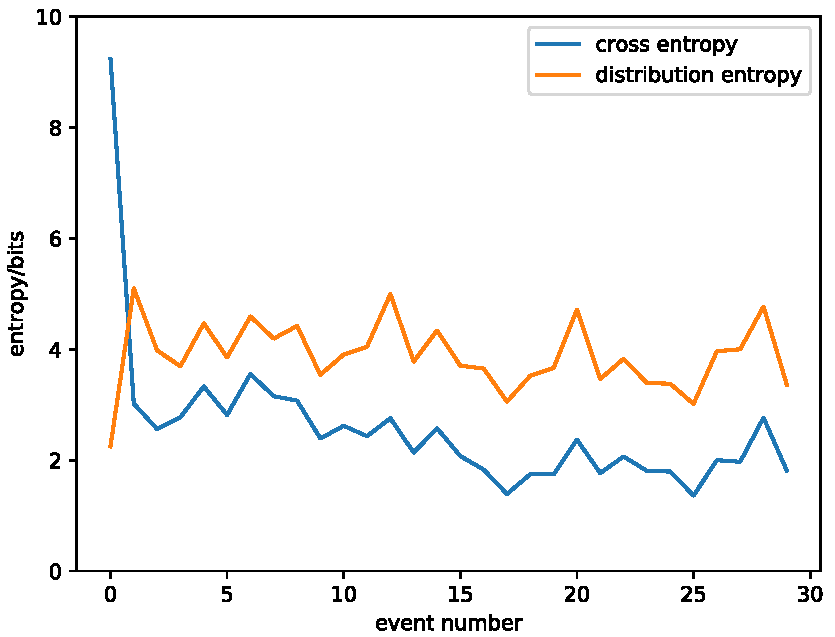
\includegraphics[width=220pt]{figs/rnn_path_profile.pdf}
}
\subfloat[MVS (mean loss: $2.248\ \mathrm{bits}$)] {
  \label{subfig:mvs-path}
  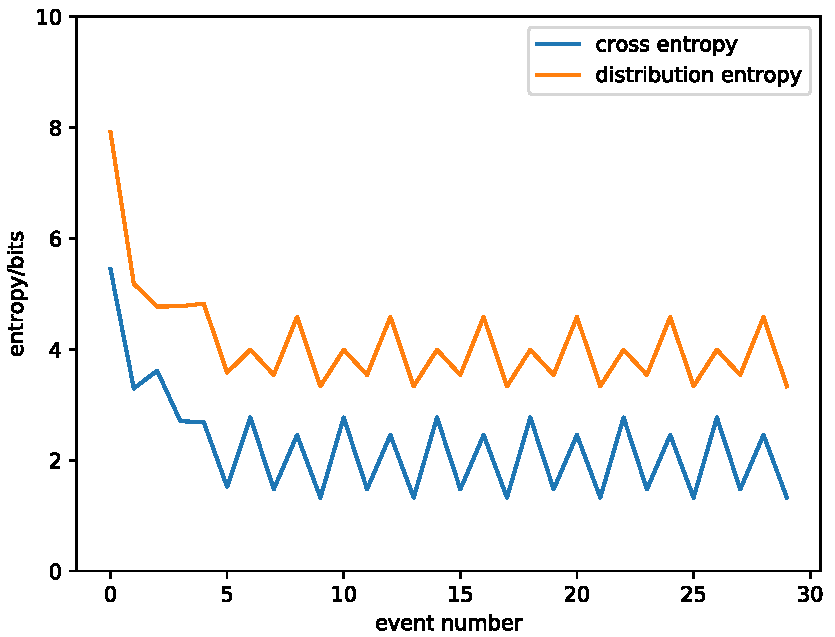
\includegraphics[width=220pt]{figs/mvs_path_profile.pdf}
}

\subfloat[Input Sequence] {
  \label{subfig:path-score}
  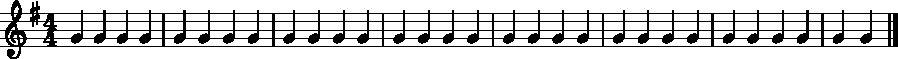
\includegraphics[width=0.85\linewidth]{figs/path_score.pdf}
}
\caption{Entropy profiles of models applied to pathalogical input}
\label{fig:path-profiles}
\end{figure}

Unfortunately, neither model rejects this input, with both assigning
cross-entropies below their respective losses on the test set. In the MVS, this
is likely due to over-fitting of the short-term model as the sequence is
predicted. The RNN exhibits similar behaviour where the cross-entropy decreases
over time. This is suggestive of an avenue for possible improvements, perhaps
utilising techniques such as \emph{negative training}.

\section{Listening Survey}

\subsection{Evaluation Criteria}

We now turn to the task of evaluating the outputs produced by sampling from the
models. To do this, we need to establish useful \emph{subjective} evaluation
criteria. Since, fundamentally, we want our models to imitate a musical style,
desirable outputs should be a \emph{pastiche} of that style. We
therefore consider the \emph{distinguishability} of our outputs from original
compositions to be a primary evaluation critereon of interest.

Secondarily, a desirable property of (arguably) \emph{any} musical composition
is that the composition is perceived as a \emph{unified} and \emph{cohesive}
whole. Often, computer-generated music is \emph{wandering} and lacking
in high-level musical structure. Therefore, we consider the perceived
\emph{coherency} of a musical composition to be a secondary critereon of
interest.

While many other criteria are of interest, we restrict our choice to these two
for the purposes of the listening survey, since the time and concentration
demands on participants should be kept to a minimum.

\subsection{Design and Implementation}

A survey for evaluating samples from the models was implemented in the form of a
web application written using the web framework Ruby on
Rails\footnote{http://rubyonrails.org/}.  The survey stored three pools of
samples: one for the MVS, another for the RNN, and a third for genuine chorale
melodies. Initially, users were asked to give a self-assessment of their musical
ability. Upon a user starting the survey, two samples would be selected from
each pool at random.  After shuffling these samples, they would be presented to
the user, at which point they were asked, for each sample:
\begin{enumerate}[label=\arabic*., itemsep=0mm]
  \item To assess whether the sample was composed by a human (i.e.\ is a genuine
    chorale) or a computer, as well as giving a confidence rating (from 0 to 4,
    expressed with English labels) for this judgement.
  \item To rate, on a Likert scale, the \emph{coherency} of the sample as a
    musical composition.
\end{enumerate}

\begin{figure}[H]
\centering
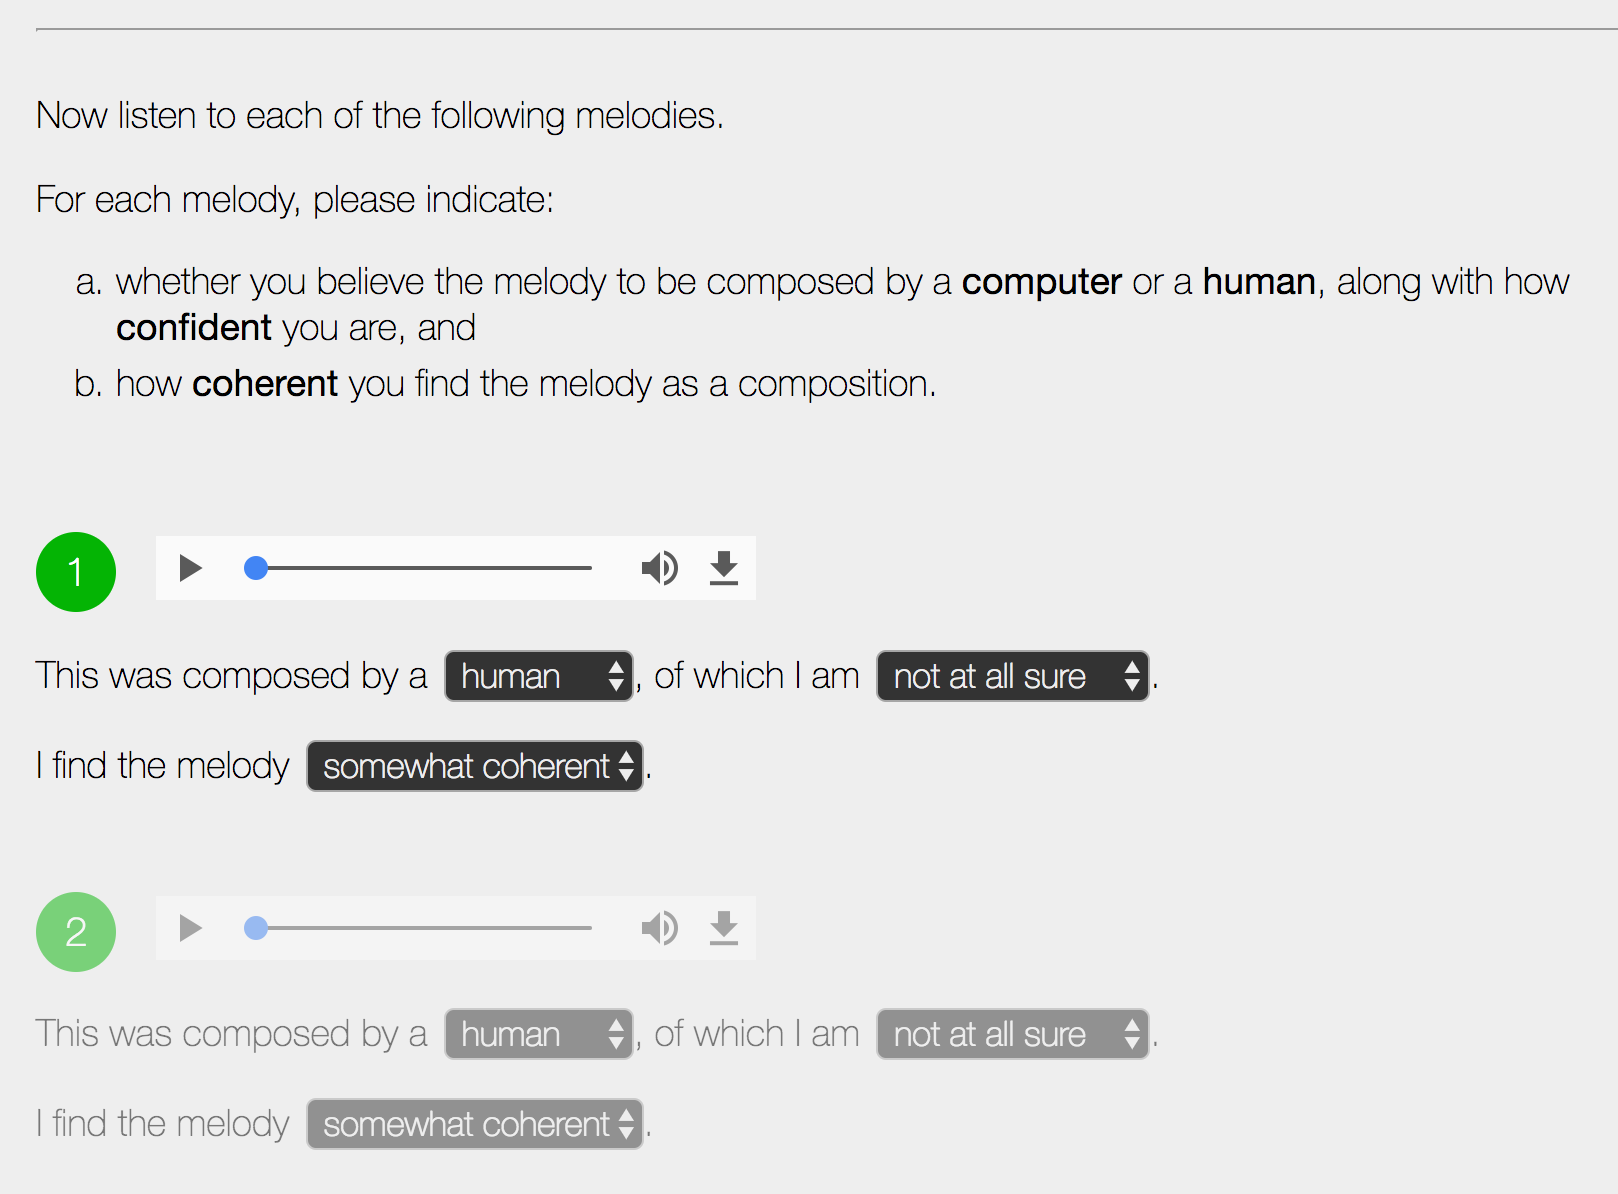
\includegraphics[width=350pt]{figs/survey_screenshot.png}
\caption{Screenshot of survey user interface}
\label{fig:survey-ui}
\end{figure}

Recent research by Liang et al.\ \cite{liangbachbot} concerning the modelling of
four-part chorales with deep recurrent networks made use of a large-scale
survey-based evaluation. A discussion with one of the authors on possible
improvements to their evaluation led to the use of a user-submitted confidence
metric for classification decisions.

Users select their musical experience from one of four categories:
\begin{enumerate}[label=\arabic*., itemsep=0mm]
  \item \emph{Novice}: Listens to music, but does not play any instruments.
  \item \emph{Intermediate}: Plays or has played an instrument, but has not
    studied composition.
  \item \emph{Advanced}: Has studied music composition in a formal setting.
  \item \emph{Expert}: Is a teacher or researcher in music.
\end{enumerate}
\vspace{2mm}

The target demographic of the survey was very broad, making the choice of online
survey appropriate. Due to the use of musical self-assessment, responses from
users across a wide spectrum of abilities were considered useful. Since the
users in the Advanced and Expert groups provide responses of the most value,
links to the survey were distributed to members of various musical groups such
as choirs and music teachers' associations. 

\subsection{Results}

In total, 102 responses were received. The distribution of users' self-assessed
experience levels is given in Figure~\ref{fig:response-dist}.

\begin{figure}[H]
\centering
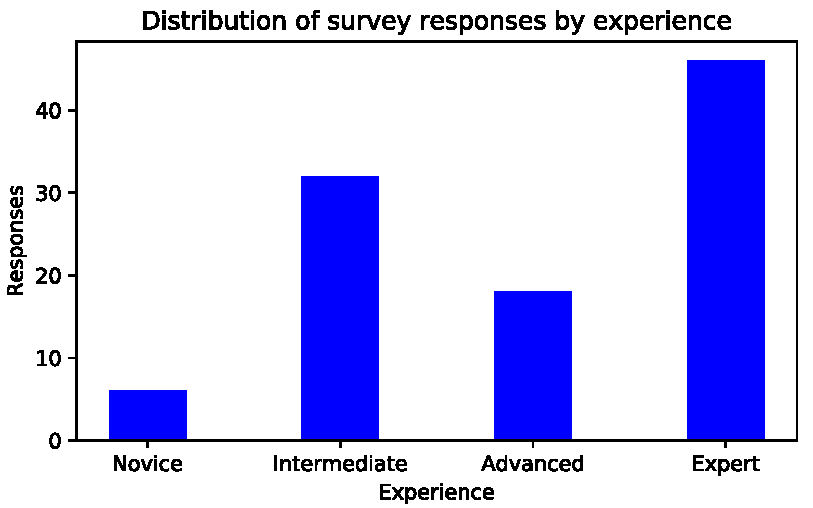
\includegraphics[width=250pt]{figs/response_dist.pdf}
\caption{User experience distribution}
\label{fig:response-dist}
\end{figure}

The primary subjective question asked of the survey participants was whether or
not they believe a sample to be composed by a human or a computer. Each such
classification was recorded along with a user-submitted confidence level on a
scale of 0-4.

Figure~\ref{fig:human-classification} summarises the user classification
results, ignoring the user-submitted confidence metric. All error bars indicate
the standard error from the mean value. We use the classifcation labels $+1$ to
indicate ``human-composed'' and $-1$ to indicate ``machine-composed''. The line
$y = 0$ in the graphs is therefore the classification performance we expect from
uninformed guessing.

\begin{figure}[H]
\centering
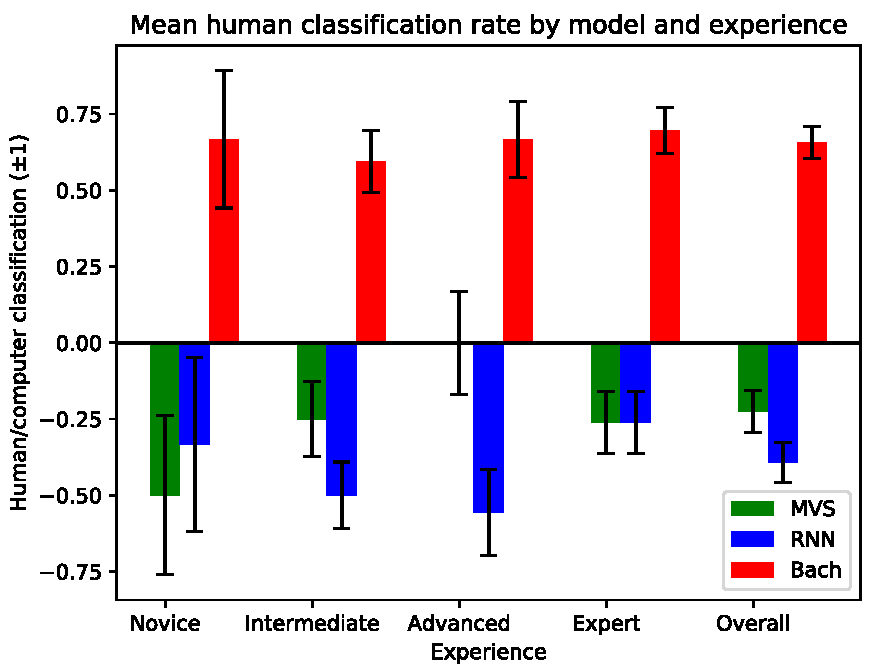
\includegraphics[width=340pt]{figs/human_classification.pdf}
\caption{Human/computer classification}
\label{fig:human-classification}
\end{figure}

Figure~\ref{fig:weighted-classification} takes the user-submitted confidence
metric into account by treating each classification as a vote, and weighting it
by the user's confidence level.
\vspace{2mm}

\begin{figure}[H]
\centering
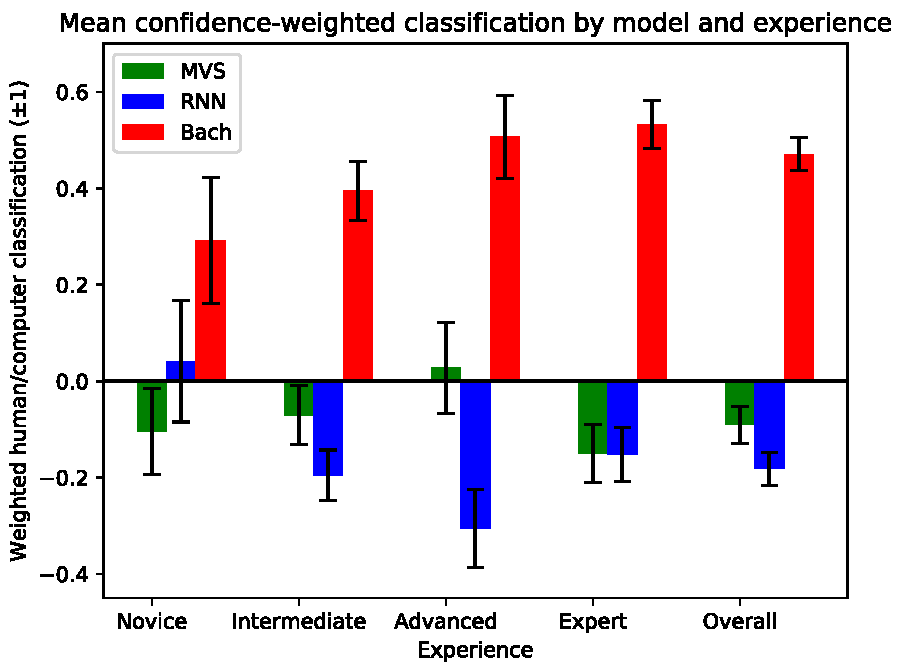
\includegraphics[width=340pt]{figs/weighted_human_classification.pdf}
\caption{Weighted classification}
\label{fig:weighted-classification}
\end{figure}
With only six Novice participants, we consider the volume of data for this class
to be insufficient. Notably, the participants who put themselves in the Advanced
category of users failed to reliably identify the MVS samples as
machine-composed, yet reliably classified the RNN samples as machine-composed.
This is especially pronounced in the confidence-weighted results. These users
also rated the MVS samples as more coherent, as shown in
Figure~\ref{fig:coherency}.

While the classification results for the Expert class are inconclusive, the
coherency ratings might indicate a slight bias towards the RNN, but this is
clearly insignificant. Looking at the aggregate results (labelled `Overall'),
while the coherency ratings are inconclusive, the classification results (both
weighted and unweighted) show that, to within one standard error, users are more
likely to label RNN samples as machine-composed and MVS samples as
human-composed.

\begin{figure}[H]
\centering
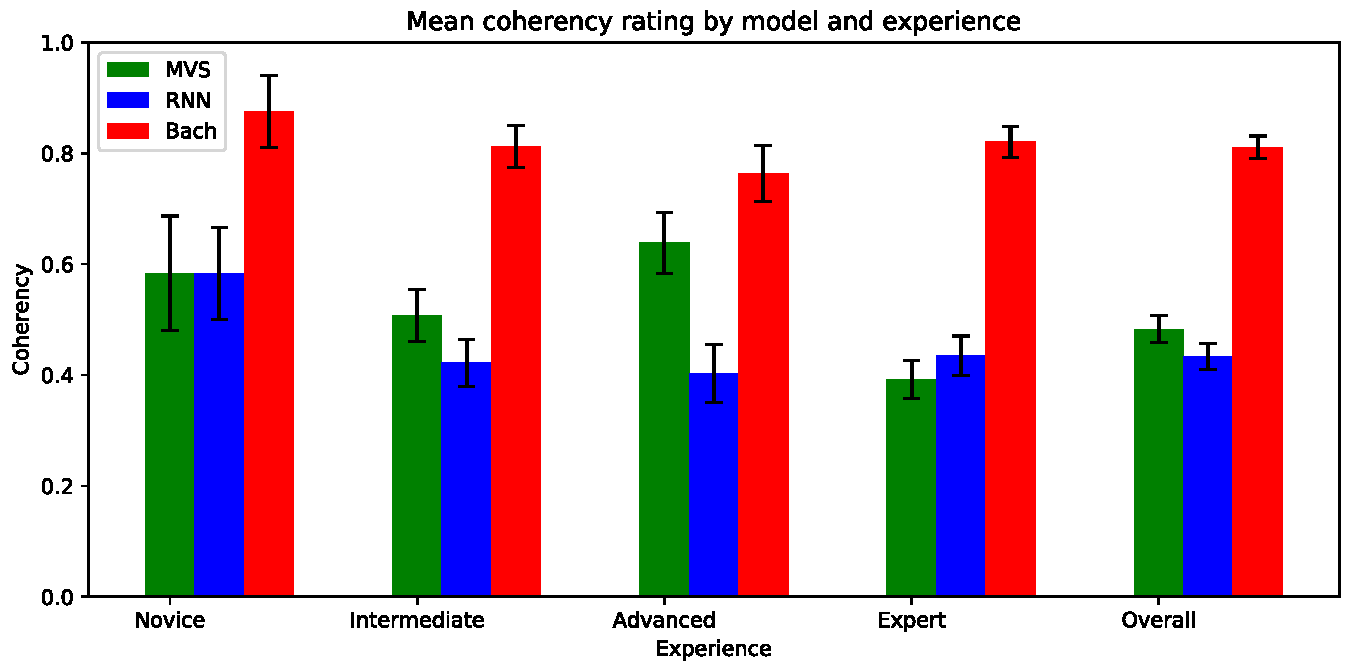
\includegraphics[width=0.75\linewidth]{figs/survey_coherency.pdf}
\caption{Coherency ratings}
\label{fig:coherency}
\end{figure}

\todo Do I need to do a sample-by-sample breakdown?

\section{Expert Evaluation}

\todo Waiting on email from Mark.

\section{Discussion}

\todo Do we need this section? Can it be the conclusion?

\chapter{Conclusion}

\todo Write me.

%%%%%%%%%%%%%%%%%%%%%%%%%%%%%%%%%%%%%%%%%%%%%%%%%%%%%%%%%%%%%%%%%%%%%
% the bibliography
\phantomsection
\printbibliography
\addcontentsline{toc}{chapter}{Bibliography}
\todo Check all the references for typos as Google Scholar certainly has a few!

%%%%%%%%%%%%%%%%%%%%%%%%%%%%%%%%%%%%%%%%%%%%%%%%%%%%%%%%%%%%%%%%%%%%%
% the appendices
\appendix

\chapter{Project Proposal}

\todo uncomment me!
%% Note: this file can be compiled on its own, but is also included by
% diss.tex (using the docmute.sty package to ignore the preamble)
\documentclass[12pt,a4paper,twoside]{article}
\usepackage[UKenglish]{isodate}
\usepackage[pdfborder={0 0 0}]{hyperref}
\usepackage[margin=25mm]{geometry}
\usepackage{graphicx}
\usepackage{parskip}
\usepackage{enumitem}
% \usepackage{mathpazo}
% \usepackage{eulervm}
\usepackage{microtype}

\usepackage[style=numeric,backend=bibtex]{biblatex}
\bibliography{refs.bib}

\begin{document}

\cleanlookdateon

\begin{center}
\Large
Computer Science Tripos -- Part II -- Project Proposal\\[4mm]
\LARGE
A Comparison of Statistical Models and Recurrent Neural Networks Applied to the
Generation of Music\\[4mm]

\large
Alex Coplan, St Catharine's College

Originator: Alex Coplan

\today
\end{center}

\vspace{5mm}

\textbf{Project Supervisor:} Matthew Ireland

\textbf{Director of Studies:} Dr S. Taraskin

\textbf{Project Overseers:} Dr M. Fiore \& Dr I. Leslie

% Main document

\section*{Introduction}

The goal of this project is to implement, evaluate, and compare two different
techniques for the algorithmic generation of music. I am particularly interested
in the generation of melody, and ultimately, \emph{polyphony}: multiple
independent melodies interacting with each other in harmonic coherence. In
particular, the two classes of techniques I intend to consider for this project
are:
\begin{itemize}[itemsep=0mm]
	\item Statistical history models such as \emph{multiple viewpoint
			systems} \cite{conklin1995viewpoints}.
	\item Recurrent neural networks.
\end{itemize}

The exact statistical model(s) to be investigated will be determined by the end
of the research phase of the project.

Algorithmic composition is of general interest in computational creativity, but
also has a number of practical applications; one such application being in
\emph{machine-assisted composition}, where a music generation tool aids a human
composer by extending or generating musical ideas. Such tools would be used by a
wide variety of music practitioners.

My intention is to undertake an investigation into the algorithmic composition
of polyphonic music. The first major problem that needs to be tackled in such an
endeavour is that of melody generation. Once this problem has been addressed,
one would subsequently consider the problem ``given a melody (the
\emph{subject}), compose a second (independent) melody (the
\emph{countersubject}) which interacts with, and is coherent with the subject.''
Since the lines in polyphony should be \emph{independent} melodies, it is
necessary to approach the problem of melody generation first.

I therefore propose that the core of the project investigate the application of
these techniques to melody generation. As an optional extension, an
investigation could then be carried out into the composition of two-part
polyphonic music, using these techniques and/or extensions thereof.

I shall follow the approach often taken in the literature of restricting the
domain of source material to stem from a particular musical idiom, e.g.\
\cite{pearce2001evaluation}. This is desirable for a number of reasons, not
least because it introduces a useful evaluation criterion: do the compositions
produced by the system exhibit a coherent musical style, consistent with that
exhibited by the material in the corpus?

In order for this project to be evaluated effectively, in addition to any
information-theoretic or music-theoretic analyses, it is necessary to perform
listening trials on human subjects. Pearce et al.\ \cite{pearce2001evaluation}
outline a framework for evaluation which allows more scientific claims to be
made as a result of the evaluation process. Evaluation would be performed in the
form of a blind trial where the subjects are asked to classify compositions as
human or machine-composed. In this work, it is noted that the participants
exhibited a bias towards classifying compositions as machine composed. This is
something that should be taken into account when designing the evaluation
methodology. An avenue for investigation in this respect is the method of
\emph{three-alternative forced choice}.

Conklin \cite{conklin2003music} notes that random walk is not necessarily the
best method of sampling from a statistical distribution such as that of a
multiple viewpoint system or Markov chain. In this project, I would therefore
also consider exploring different techniques for sampling from statistical
models.
 
\subsection*{Background}

Markov processes are natural statistical models for the analysis of melody, and
are well known as tools for composition \cite{ames1989markov}. Although
effective, Markov processes are far from perfect tools for modelling music.
Specifically, a basic pitch-duration Markov process disregards a considerable
amount of musical information available in the context
\cite{conklin1995viewpoints}.  

However, simply incorporating more musical features into the state space of a
Markov chain leads to an exponential blow-up in space complexity and
necessitates both a large amount of training data for good performance, as well
as solving the sparse data problem (\cite{conklin2003music}, section 2.1).
Moreover, Markov chains do not make use of the long-term context of a system,
which is necessary for modelling the broader sense of sequence and structure
which is present in music.

Conklin et al.\ \cite{conklin1995viewpoints} introduce the method of
\emph{multiple viewpoints} which uses the interpolation of the predictions of
many different context models, each of which considers a different musical
attribute (or some combination of attributes). These include both short-term and
long-term attributes, enabling this method to capture sequence and structure.

It is well known that Recurrent Neural Networks (RNNs) can effectively generate
sequences. RNNs have seen more successful application in music following the
introduction of long short-term memory (LSTM) techniques \cite{eck2002lstm}.
Without use of LSTM, RNNs exhibit similar problems to Markov chains in that the
output does not contain the elements of sequence and structure that one might
expect from compositions in the corpus.

\section*{Starting point}

In Lent term of 2016, I gave a talk (as part of Churchill college's Computer
Science talk series) on melody generation using Markov chains. I also
constructed a demo in Ruby which implemented a parser for ABC
notation\footnote{\url{http://abcnotation.com/}} along with a simple Markov
chain model, trained of a small corpus of hymn tunes, which generated tunes by
random walk. 

Although this experience led me to this choice of project, the implementation of
a model such as a multiple viewpoint system is considerably more involved, and
the architecture vastly different. The implementation of this model will
therefore be carried out from scratch.  The neural network will be implemented
using a library such as Google's
TensorFlow\footnote{\url{https://www.tensorflow.org/}}.

As an organ scholar (and previously an A-Level music student), I have
considerable experience with performing polyphonic music (and some experience of
analysis), especially that of the renaissance and baroque eras. I believe this
domain knowledge will prove especially useful for making musically-informed
decisions in this project. 

\section*{Resources required}

For this project I shall primarily use my own laptop. Backup will be primarily
in the form of a GitHub-hosted repository, but I will also perform backups of
the project files to an external hard drive as well as multiple cloud providers
(Google, Apple, Dropbox) and the MCS. Should my main computer suddenly fail, I
can easily continue the project using MCS computers by cloning the code from the
GitHub repository.

Although datasets can easily be compiled from online sources, it may also be of
use to have a MIDI keyboard to be able to input arbitrary musical data. I own a
MIDI keyboard which would be suitable for these purposes. I will make use of
open-source software (such as MuseScore\footnote{\url{https://musescore.org/}})
for synthesis of MIDI and other musical data. I require no other special
resources.

\section*{Work to be done}

I will employ an agile software development methodology when undertaking this
project. The ordered list of sub-tasks within this project are:
\begin{enumerate}

\item Devising and implementing an internal representation of musical data,
	along with a simple ``music theory engine'' to process this data.  

\item Implementing a simple parser for some form of input notation (ABC, MIDI,
	MusicXML); the exact form to be determined in the research phase.  

\item Implementing and iteratively refining the statistical model (e.g. multiple
	viewpoint system).

\item Implementing and iteratively refining the RNN for melody generation.  

\item Designing and carrying out a scheme for human evaluation.

\item Making iterative improvements to the two models.

\end{enumerate}

\section*{Success criteria}

\subsection*{Core Tasks}

The project will be a success if I have:
\begin{itemize}
	\item Successfully implemented a statistical model such as a multiple
		viewpoint system capable of generating melody.
	\item Successfully implemented a technique based on recurrent neural
		networks capable of generating melody.
	\item Performed an evaluation and comparison of the two
		models, answering questions such as:
	\begin{itemize}
		\item Can human subjects distinguish the machine-composed output
			from the human-composed samples in the corpus?
		\item Do human subjects classify the machine-composed output as
			adhering to the specified style?
	\end{itemize}

	Note that the success of the evaluation stage is not predicated on the
	answers to the questions given above, but merely whether the evaluation
	is conducted in a scientific manner.
\end{itemize}

\subsection*{Extension Tasks}

The project will be judged as a success if all the core tasks have been
completed. The extension tasks won't be used to judge the success of the
project, but it will have gone above and beyond expectations if one of them is
completed.

These possible extensions include:
\begin{itemize}
	\item Extending a multiple viewpoint system to generate polyphony.
	\item Extending a RNN to generate polyphony.
	\item Exploring extensions and adaptations of multiple viewpoint
		systems.
\end{itemize}

\section*{Timetable}

Planned starting date is 16/10/2011.

\begin{tabular}{ p{4cm} | p{11cm} } \hline 
% TODO: 2 week blocks, start earlier to include proposal week.
% TODO: 2-page spread

16/10/16 - 27/10/16 Mich. Weeks 2-4 & \textbf{Research phase}.
Research multiple viewpoint systems, RNNs, and evaluation techniques.
Investigate options for corpus material and format. This will inform the type of
parser that should subsequently be implemented. Devise and fix an internal
representation for musical data. Design specific multiple viewpoint system based
on \cite{whorley2013phd}. The corpus should also be prepared as fully as
possible during this stage. Familiarisation with libraries (e.g. TensorFlow)
should be accomplished during this phase.

\textbf{Milestone}: Report summarising research handed to supervisor.
\\ \hline
03/11/16 - 10/11/16 \newline Mich. Week 5 & \textbf{Preliminary Implementation}. 
Implement parser for chosen corpus format. Implement internal representation as
determined in the previous phase. Write test suite for the above. 
\\ \hline
10/11/16 - 30/11/16 \newline Mich. Weeks 6-8 & \textbf{MVS Implementation I}.
First iteration of multiple viewpoint system to be completed in these three
weeks. System need not be complete in terms of the exact viewpoints used.
However, the underlying machinery should be. In particular, context models,
viewpoint representation, prediction interpolation etc. should all be
implemented, such that a MVS can be constructed, trained, and used for
generation.
\\ \hline
01/12/16 - 22/12/16 \newline Christmas Vac. Weeks 1-3 & \textbf{RNN Implementation I}.
Implement LSTM Recurrent Neural Network. 
\\ \hline
29/12/16 - 12/01/17 \newline Christmas Vac. Weeks 4-5 & \textbf{MVS Implementation II}.
Implement full multiple viewpoint system. Investigate different choices of
viewpoints as per the R\&D outlined in the research phase. 
\\ \hline
12/01/17 - 26/01/17 \newline Lent Week 0 & \textbf{RNN Implementation II}.
Finish RNN implementation. Train network on entire corpus.
\\ \hline

\end{tabular}

\printbibliography

\end{document}


\end{document}
